\documentclass[11pt]{article}
\usepackage[sc]{mathpazo} %Like Palatino with extensive math support
\usepackage{fullpage}
%\usepackage[authoryear,sectionbib,sort]{natbib}
\linespread{1.7}
\usepackage[utf8]{inputenc}
\usepackage{lineno}
\usepackage{titlesec}
\usepackage{graphicx} %added
\usepackage{amsfonts} %added
\usepackage{amsmath} % added
\usepackage{float} % added
\usepackage{amssymb} %added
\usepackage{longtable} % added
\usepackage{booktabs} % added
\usepackage{caption}
\usepackage{xurl}
\usepackage{lscape}
\usepackage{multirow}
\captionsetup{labelformat=empty}
\usepackage{makecell} % added
\usepackage{adjustbox} % added
\titleformat{\section}[block]{\Large\bfseries\filcenter}{\thesection}{1em}{}
\titleformat{\subsection}[block]{\Large\itshape\filcenter}{\thesubsection}{1em}{}
\titleformat{\subsubsection}[block]{\large\itshape}{\thesubsubsection}{1em}{}
\titleformat{\paragraph}[runin]{\itshape}{\theparagraph}{1em}{}[. ]\renewcommand{\refname}{Literature Cited}
\usepackage[font=small,labelfont=bf]{caption}%added
%%%%%%%%%%%%%%%%%%%%%
% Line numbering
%%%%%%%%%%%%%%%%%%%%%

\title{Supplementary Information for \emph{A highly-resolved food web for insect seed predators in a species-rich tropical forest}}

% This version of the LaTeX template was last updated on
% January 11, 2018.

%%%%%%%%%%%%%%%%%%%%%
% Authorship
%%%%%%%%%%%%%%%%%%%%%
% Please remove authorship information while your paper is under review,
% unless you wish to waive your anonymity under double-blind review. You
% will need to add this information back in to your final files after
% acceptance.
\author{S. Gripenberg \emph{et al.}}



\date{}

\begin{document}

\maketitle


\tableofcontents


\newpage

\section{Appendix S1: Supplementary methods}

\subsection*{Processing the insect material to obtain (morpho)species identifications}

When encountered in rearing pots, adult Coleoptera, Diptera and Hymenoptera were transferred to vials with ethanol, while Lepidoptera were spread and dried. Where insects (typically weevils) emerged from the seed and fruit samples as larvae, they were stored in 95\% ethanol to allow molecular identification through DNA barcoding (Hebert \emph{et al.}2003). Where multiple similar-looking larvae were encountered in the same rearing pot on the same day they were assumed to belong to the same species. In such cases, one individual was stored in ethanol while remaining larvae were placed in pots with sterilised soil in an attempt to rear adults for morphology-based identification. Many (72.5\%) of the 1889 larvae placed in soil pots did not emerge as adults. The likely species identity of these larvae – and of larvae in ethanol that were not DNA barcoded – was inferred from the DNA barcode of the paired larval samples stored in ethanol or from the identity of any adults emerging from the same soil pot. 

All adult insects emerging from seeds or soil were assigned to a morphospecies based on their morphology. Initially, insect specimens reared from different plant species were processed separately and given different morphospecies-by-plant species codes. These were later merged to true species (or morphospecies) based on examination of selected specimens by experts on each taxonomic group. To ensure that the material did not include cryptic species (e.g. Hebert \emph{et al. }2004), up to 5 individuals per morphospecies excluding Hymenoptera (a total of 2733 adults and 244 larvae) were DNA barcoded (i.e. the mitochondrial COI gene sequenced; Hebert \emph{et al. }2003). DNA sequencing of adult specimens was done at the Biodiversity Institute of Ontario using their standard protocols and primers (Wilson 2012). DNA barcoding of larvae was done by Eero Vesterinen at the University of Turku. Barcode Index Numbers (Ratnasingham \& Hebert 2013) were obtained for 35.8\% of the (morpho)species in the full material and for 72.3\% of the (morpho)species classified as seed predators (see below). In most cases there was a close match between our initial morphospecies codes and the DNA barcodes, although in a few cases (notably within the Bruchinae), species assignments based on morphological characters proved difficult for non-specialists.

\subsection*{Assigning insect species and morphospecies to feeding guild}

The seed and fruit samples inevitably yielded some insects that were not true seed predators, but pulp feeders, scavengers or fungivores, as well as natural enemies (parasitoids) associated with seed predators or members of the above-mentioned feeding guilds. In the context of the current study, we were exclusively interested in insects that are true seed predators, i.e. those that suppress the reproductive output of their hosts by killing seeds. Based on information about the ecology of different taxa, our own observations, and discussions with experts on different taxonomic groups, each insect species was assigned to its most likely feeding guild (seed predator versus other), following the principles outlined below:
Of the Coleoptera, all bruchids (Bruchinae), Curculionidae (with the exception of Scolytinae; see below) and longhorn beetles (Cerambycidae) were classified as seed predators. While the majority of Scolytinae are likely to be pulp feeders or feeding on endocarps or the woody parts of fruits, one species (\emph{Pagiocerus frontalis}) was classified as a seed predator based on clear evidence of feeding damage on the seeds of all of its documented host species (S. Gripenberg, \emph{pers. obs.}). 
In terms of Lepidoptera, all members of the families Cosmopterigidae, Crambidae, Heliodinidae, Oecophoridae, Pyralidae, Sesiidae and Tortricidae were assumed to be seed predators. Based on expert opinion (Robert Robbins, \emph{pers. comm.}) and feeding damage observed to seeds, three genera of Lycaenidae (\emph{Strymon}, \emph{Strephonota} and \emph{Tmolus}) were assigned as seed predators. Tineidae were assumed to be scavengers, although the family includes diverse larval habits (Robinson 2009). Blastobasidae are historically assumed to be scavengers, although some species may feed on living tissue in fruits (Adamski \emph{et al. }2010).
Most Hymenoptera reared from our samples are likely to be parasitoids of seed and fruit eating insects. Members of two families (Agaonidae and Eurytomidae) were labelled as seed predators based on what is known about their feeding habits in other contexts (Donald Quicke,\emph{ pers. comm.}). 
In terms of Diptera, we recognise that some species reared from our seed and fruit samples (notably members of the families Tephritidae and Lonchaeidae) are likely to be seed predators. Nevertheless, since our data do not allow us to confidently assign individual dipteran species to the correct feeding guild we have refrained from including this species-rich order in our analyses. It will, however, be included in future analyses focusing on the wider insect communities associated with seeds and fruits (Basset \emph{et al.}, in prep.).
Overall, we believe our criteria for assigning species to feeding guild are strict: it is more likely that we have excluded seed predators than included non-seed predating species in our analyses. We note that there is a possibility that some seeds attacked by species scored as seed predators might still be viable (e.g. \emph{Prioria copaifera} seeds with signs of insect seed predator attack have been observed to germinate; Dalling \emph{et al. }1997). Nevertheless, in the vast majority of interactions documented in this study, we believe the effect of the insects scored as seed predators to be lethal. 

\subsection*{Details on analyses testing for phylogenetic signal}

The $D$ statistic (Fritz \& Purvis 2010) which was used to test for phylogenetic signal in the incidence of seed predators across the plant community assesses the sum of changes in estimated nodal values of a binary trait across a phylogeny. The value of $D$ was compared to $D$ values found under models of phylogenetic randomness and evolution under Brownian motion. $D$ values significantly smaller than 1 indicate that the examined trait is phylogenetically clumped and $D$ values equal to 0 suggest that the trait is as clumped as if it had evolved under Brownian evolution. Whether observed $D$ values deviated significantly from 1 and 0 was assessed using 1000 simulations (for details, see Fritz \& Purvis 2010). Analyses were conducted for all seed predator taxa combined, and for each order (Coleoptera, Lepidoptera, Hymenoptera) separately.
We tested for phylogenetic signal in seed predator richness and seed predation rates using Blomberg’s $K$ (Blomberg \emph{et al. }2003). To obtain P-values associated with $K$, we used the R package phytools (Revell 2012). To minimise potential issues resulting from variable sample sizes and incomplete sampling, only plant species with a minimum sample size of 200 seeds/fruits were included in the analyses on phylogenetic signal.

Details on random forest analyses relating plant traits to seed predation
Data were collated from a number of different sources, listed in Appendix S2. When assessing seed predation rate, we excluded plant species with seeds smaller than 1 mg, since our observations suggested that seeds smaller than this are likely to be too small to be attacked by endophagous seed predators. Amongst the well-sampled plant species ($\geq$200 seeds/fruits) upon which we focussed our main analyses, the trait data completeness was above 50\% for all the variables tested (Table S1.1). Missing values are dealt with by the default approach of the cforest() function, which uses surrogate splits where necessary (Hothorn \emph{et al. }2006). 

\begin{table}[]
\small
\begin{tabular}{@{}lll@{}}
\toprule
Trait                           & Well-Sampled Missing \% & All Data Missing \% \\ \midrule
Lifeform                        & 0.0                     & 0.8                 \\
BCI genus-level diversity       & 3.3                     & 7.3                 \\
BCI family-level diversity      & 8.0                     & 6.1                 \\
Overlap in fruit production     & 8.5                     & 26.7                \\
Seed dry mass                   & 14.6                    & 30.7                \\
Endocarp investment             & 14.6                    & 30.1                \\
Local Seed crop size            & 28.6                    & 52.0                \\
Interannual crop size variation & 30.0                    & 53.0                \\
Tree height                     & 34.3                    & 50.5                \\
Local Abundance                 & 34.7                    & 51.1                \\
Relative Growth Rate            & 48.8                    & 67.4                \\
Polyphenol concentration        & 49.8                    & 70.8                \\ \bottomrule
\end{tabular}
\caption{\textbf{Table S1.1} Fraction of missing data for each trait in the plant dataset. }
\label{tab:my-table}
\end{table}

Correlations between traits were generally low (Figure S1.1). The principal exception was seed crop variables (crop size, crop variation and fruit production overlap) that formed a distinct cluster. 
We sought to determine if a wide suite of traits could allow the prediction of our seed predator response variables with random forest models. This type of model builds a collection of classification or regression trees to improve performance. The specification of random forest models can be altered by a wide range of ‘hyperparameters’, including the number and depth of classification trees and how the model’s performance is tested. The results that we present made use of the default settings of the \texttt{cforest()} function in the party package (Table S1.2) with one exception: the number of trees per model was increased to 5000. While exploring the data we tested a wide variety of different combinations, as well as other random forest modelling frameworks, but there was little meaningful improvement. Model performance was tested with out-of-bag testing. In this approach a model is fit using all-but-one result, and the ability to fit the sample left out is examined.



\begin{figure}[H]
\centering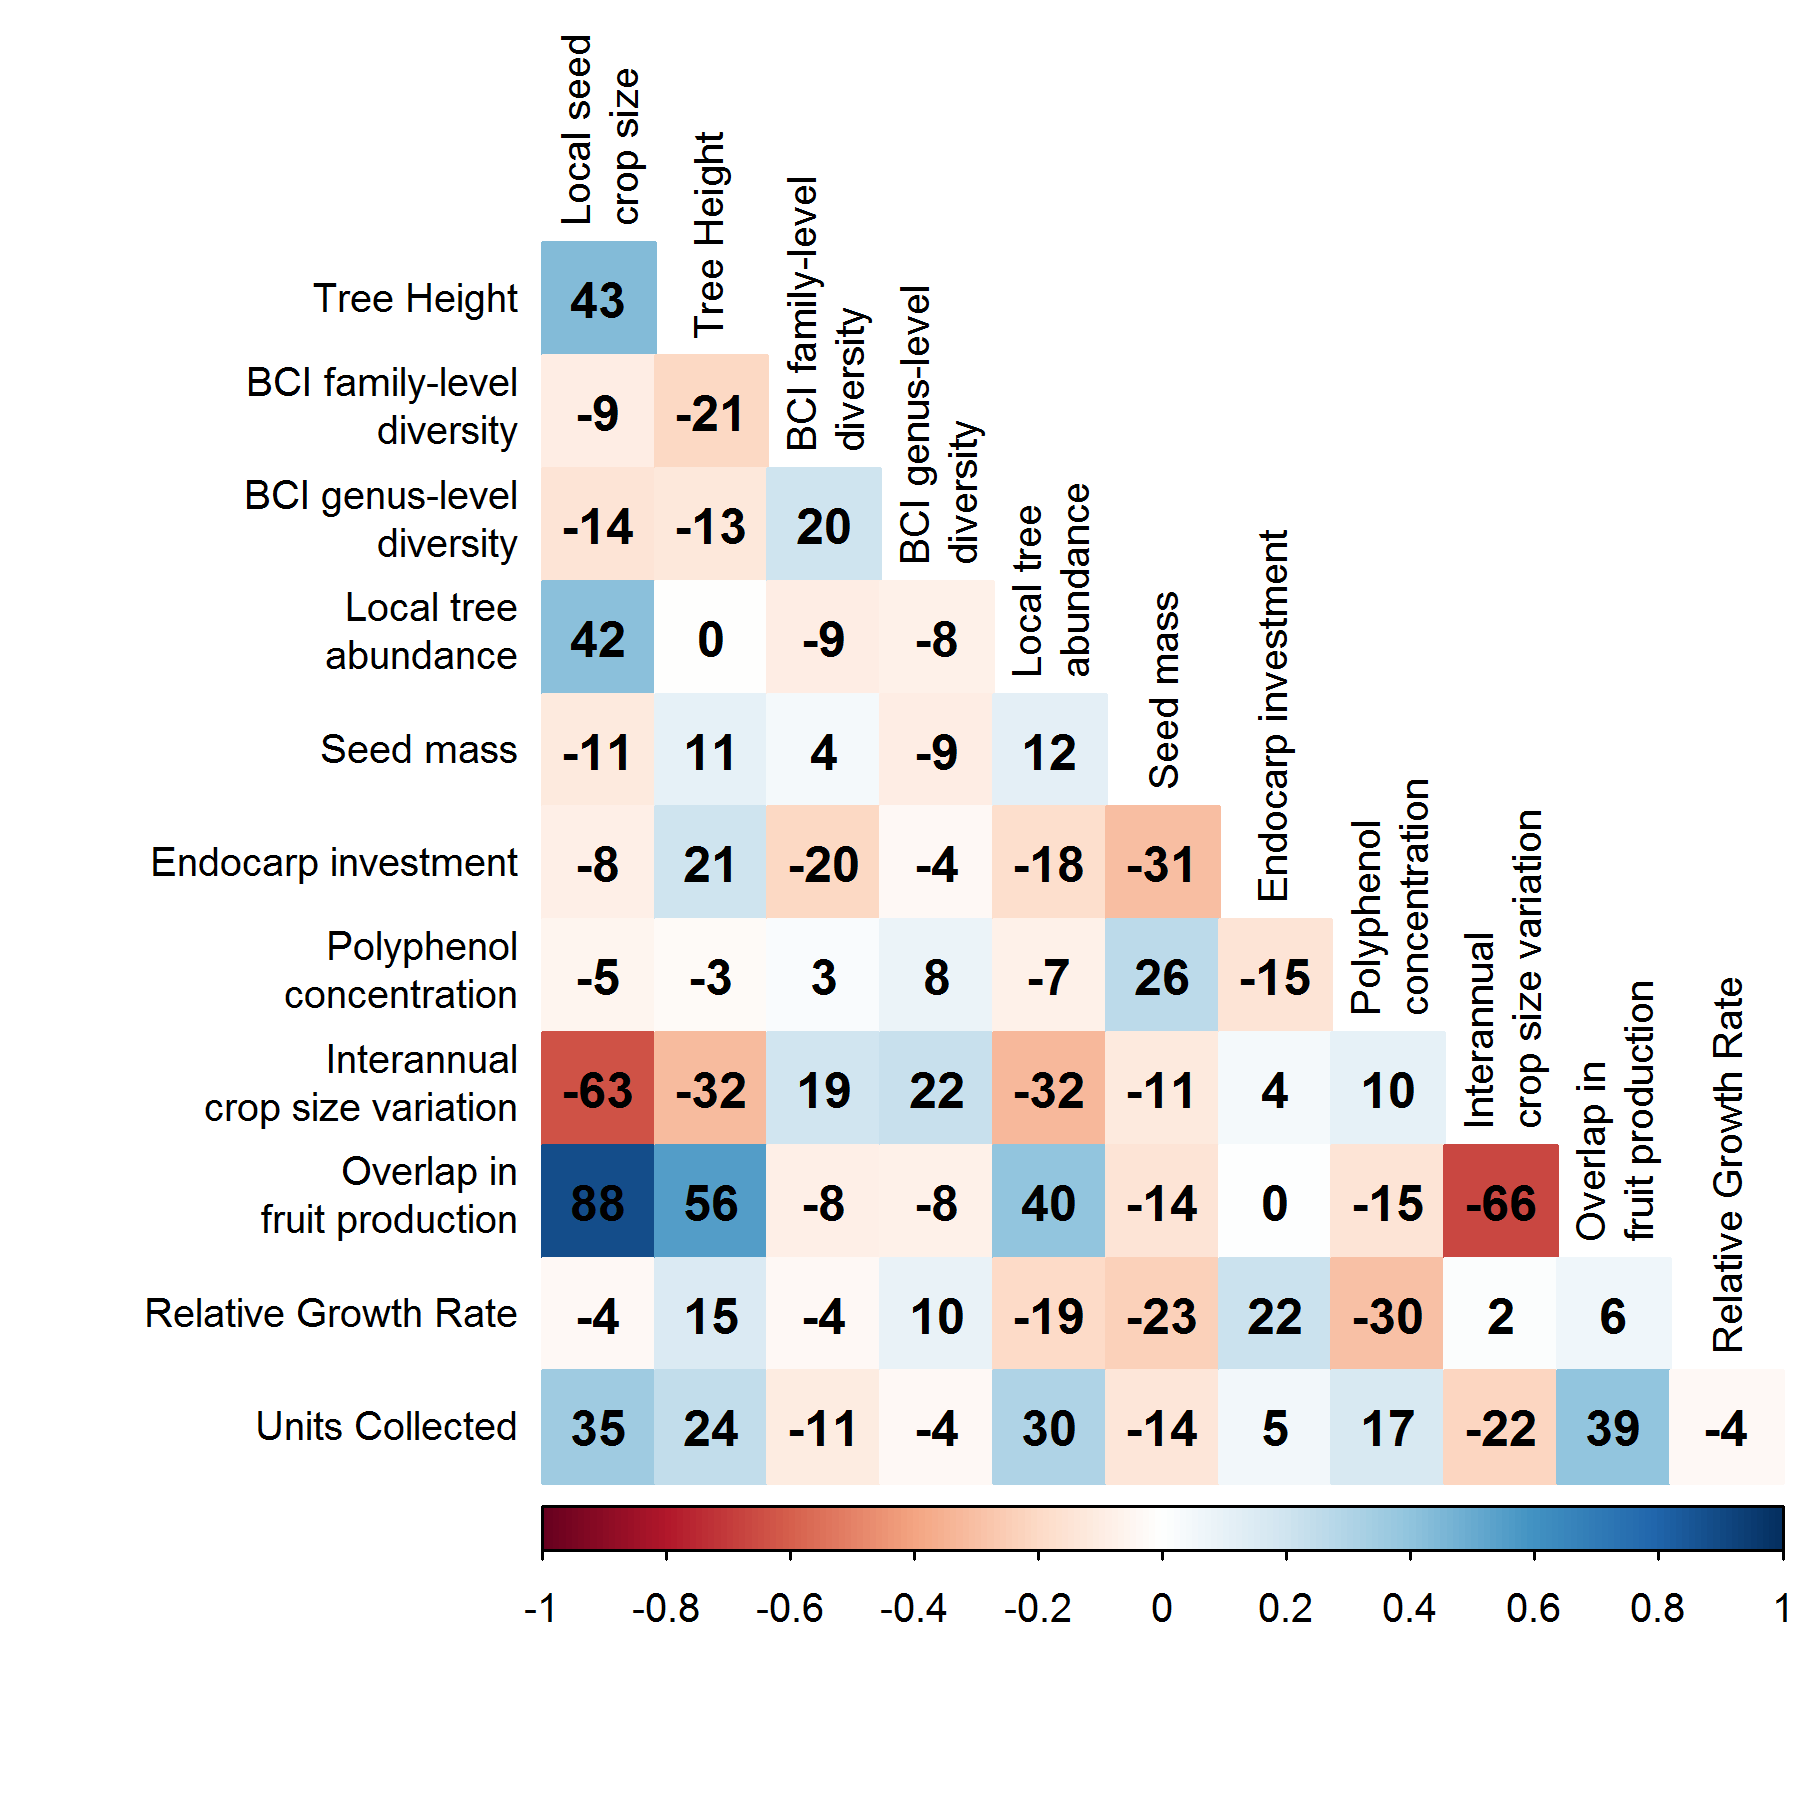
\includegraphics[width=0.7\textwidth]{../Figures/TraitCorrelation.png} 
\caption[]{ \textbf{Figure S1.1.} Correlations between the numeric continuous seed traits and sample size. Numbers and colour show Spearman’s rank correlation coefficient (rescaled to percentages for conciseness). }
\end{figure}


\begin{table}[]
\small
\begin{tabular}{@{}lp{2in}l@{}}
\toprule
Setting name in cforest() & Explanation                                                                & Value                   \\ \midrule
mtry                      & The number of variables to use in each tree                                & 5                       \\
ntree                     & The number of classification or regression trees to include in each model  & 5000                    \\
mincriterion              & The value of the test statistic that must be exceeded to implement a split & 0 (i.e unbounded trees) \\ \bottomrule
\end{tabular}
\caption{\textbf{Table S1.2} Values of hyperparameters used for reported results. }
\end{table}

Comparing the role of different variables in driving the accuracy of predictions is challenging in a random forest model, especially when the variables have differing levels of missingness, are sometimes categorical and may be somewhat correlated. Variable importance measures examine the mean decrease in accuracy if a predictor variable is randomised. To gain some insight into the driving features of our model we used the \texttt{varimp()} function in the party package. Since our data had a number of missing values, we used the approach detailed in Hapfelmeier \emph{et al. }(2014).


\subsection*{Details on the estimation of species-specific seed abundances for the quantitative food web}

Species-specific seed abundances were estimated based on a data set of seeds (or individual diaspores) and fruits (i.e. seed-bearing structures with one or more seeds) collected from a network of 200 seed traps (each 0.5m$^2$ in size) in the 50-ha Forest-GEO forest dynamics plot (Anderson-Teixeira \emph{et al. }2015) on a weekly basis from 1987 to 2015. For each species, the total counts of the following seed and fruit parts falling into the traps were recorded: \emph{mature fruits}, \emph{single diaspores} (i.e. `seeds’), \emph{capsules} (part that vertebrates never eat; botanically this might be a capsule, pedicel, bract, etc.), \emph{fragments of fruit} dropped by vertebrates (the number of fruit represented was recorded by counting pedicels or the points of attachment to the mother plant), \emph{immature fruits }(endosperm of seeds is not filled), \emph{fruit with insect emergence hole} (only recorded for selected species), \emph{aborted fruits} (fall soon after flowering, have a swollen ovule, and often have some flower parts attached), \emph{fruit eaten by animal}. To estimate the total number of seeds produced for each species, we multiplied the number of fruits collected by the species-specific average number of seeds per fruit, and then added \emph{either} the number of seeds \emph{or} the number of capsules multiplied by species-specific average number of fruits per capsule multiplied by average number of seeds per fruit; whichever number was larger. The rationale for this approach is that since some of the seeds falling into the trap might have originated from the capsule, we might overestimate seed numbers if we were to use (fruits $\times$ average seeds/fruit) + seeds + (capsules $\times$ average seeds/fruit). Since many seed predators are likely to be pre-dispersal seed predators attacking the fruits before they reach maturity, immature fruits were included in the estimates.

For the majority (77.6\%) of species, information on the typical number of seeds per fruit was obtained from fruit dissections carried out on BCI in the context of other research projects (S. J. Wright, unpubl. data). For remaining species, information on typical seed numbers per fruit was extracted from Croat (1978). (Where a range of seed numbers per fruit was reported for a species, we used the median value of this range.) For a small number of species (n=27) for which data on seed numbers per fruit were missing but for which there was information on seed numbers per fruit for congeneric species, we used the genus-specific average number of seeds per fruit (obtained from the above-mentioned sources). Following these approaches, we obtained an estimate for number of seeds per fruit for all but 11 species (3.1\%) in the food web data set. We note that the species for which data on seeds per fruit were missing were typically berries, which were excluded from the food web for other reasons (estimating the proportion of seeds killed by seed predators was not possible for these species; see main text).  

\subsection*{References for Appendix 1}

\begin{enumerate}
\item Adamski, D., Copeland, R.S., Miller, S.E., Hebert, P.D.N., Darrow, K. \& Luke, Q. (2010). A review of African Blastobasinae (Lepidoptera: Gelechioidea: Coleophoridae), with new taxa reared from native fruits in Kenya. Smithsonian Contributions to Zoology, 1-68.
\item Anderson-Teixeira, K.J., Davies, S.J., Bennett, A.C., Gonzalez-Akre, E.B., Muller-Landau, H.C., Wright, S. J. \emph{et al. }(2015). CTFS-ForestGEO: a worldwide network monitoring forests in an era of global change. Global Change Biology, 21, 528-549.
\item Blomberg, S.P., Garland, T. \& Ives, A.R. (2003). Testing for phylogenetic signal in comparative data: behavioral traits are more labile. Evolution, 57, 717-745.
\item Croat, T.B. (1978). Flora of Barro Colorado Island. Stanford University Press.
\item Dalling, J.W., Harms, K.E. \& Aizprúa, R. (1997). Seed damage tolerance and seedling resprouting ability of Prioria copaifera in Panamá. J. Trop. Ecol., 13, 481-490.
\item Fritz, S.A. \& Purvis, A. (2010). Selectivity in mammalian extinction risk and threat types: a new measure of phylogenetic signal strength in binary traits. Conserv. Biol., 24, 1042-1051.
\item Hapfelmeier, A., Hothorn, T., Ulm, K., \& Strobl, C. (2014). A new variable importance measure for random forests with missing data. Statistics and Computing, 24, 21–34.
\item Hebert, P.D., Cywinska, A. \& Ball, S.L. (2003). Biological identifications through DNA barcodes. Proc. R. Soc. Lond. B: Biol. Sci., 270, 313-321.
\item Hebert, P.D.N., Penton, E.H., Burns, J.M., Janzen, D.H. \& Hallwachs, W. (2004). Ten species in one: DNA barcoding reveals cryptic species in the neotropical skipper butterfly Astraptes fulgerator. Proc. Natl. Acad. Sci. U. S. A., 101, 14812-14817.
\item Hothorn, T., Hornik, K. \& Zeileis, A. (2006). Unbiased recursive partitioning: A conditional inference framework. J. Comp. Graph. Stat., 15, 651-674.
\item Ratnasingham, S. \& Hebert, P.D.N. (2013). A DNA-Based Registry for All Animal Species: The Barcode Index Number (BIN) System. PloS One, 8, e66213.
\item Revell, L.J. (2012). phytools: an R package for phylogenetic comparative biology (and other things). Meth. Ecol. Evol., 3, 217-223.
\item Robinson, G.S. (2009). Biology, Distribution and Diversity of Tineid Moths. Southdene, Kuala Lumpur.
\item Wilson, J.J. (2012). DNA barcodes for insects. In: DNA Barcodes: Methods and Protocols (eds. Kress, WJ \& Erickson, DL). Springer New York, pp. 17-46.
\end{enumerate}



\newpage

\section{Appendix S2: Origins of data sets on plant traits}

The data sets needed to assess the relationship between community-level patterns of seed predator attack (incidence of seed predators, seed predator richness, and proportion of seeds scored as predated) and traits hypothesised to make plant species more or less prone to seed predation (Table 1 in the main text) were obtained from a variety of sources:
 
\textbf{Local seed abundance} – Data used to quantify seed abundances of individual tree and liana species in the BCI community were obtained from S. J. Wright’s long term study focusing on seed rain into a network of 200 seed traps (0.5 m2) located in the 50-ha forest dynamics plot on BCI (see e.g. Harms \emph{et al. }2000, Wright \emph{et al. }2005). For the species encountered in the seed traps, species-specific seed production was taken as a measure of seed abundance at the community level. Seed production was calculated by summing the counts of seeds falling into the seed traps during the period between January 1987 and October 2010.

\textbf{Maximum tree height} – Data on the maximum height (m) of trees were collected using methods described in Wright \emph{et al. }(2010).

\textbf{Confamilial species on BCI} – For each sampled plant species, information on the number of plant species within the same family known to occur on BCI was obtained from a list of plant species recorded on BCI compiled by Carmen Galdames.

\textbf{Congeneric species on BCI} – Information on the number of plant species within the same genus known to occur on BCI was obtained from a list of plant species recorded on BCI compiled by Carmen Galdames.

\textbf{Local abundance of adult trees }– The local abundance of reproductive-sized adult trees was estimated using data from the 2010 census of the ForestGeo plot (Condit 1998, Hubbell \emph{et al. }1999, Hubbell \emph{et al. }2005). To estimate the number of reproductive adults in the 50-ha plot, we extracted species-specific maximum diameter at breast height (DBHmax) and selected all individuals with a DBH larger than 0.5 $\times$ DBHmax (the known size threshold for tree reproduction; Visser \emph{et al. }2016).

\textbf{Seed mass} – Species-specific seed masses were available in the form of mean dry seed mass (expressed in grams) where a `seed' is defined to include the endosperm and embryo only. For the majority of species, the mean seed mass was based on an average of 5 seeds collected from 5 individuals and dried to constant mass at 60$^{\circ}$C (for some species, sample sizes were slightly lower). 

\textbf{Endocarp investment} – To obtain a measure of the degree of investment in mechanical seed defences, we used a largely unpublished data set on species-specific protective tissue content, reflecting the proportion of diaspore mass made up by protective tissue (e.g. endocarps and seed coats) rather than seed mass. These data were obtained by dissecting diaspores into three parts: seed (embryo plus endosperm only), appendages to enable dispersal by wind (wings for virtually all species), and material to protect the seed. All material was oven dried at 60$^{\circ}$C for at least 72 hours and then weighed for dry mass. The protective tissue content was taken as the dry weight of the seed protection material divided by the diaspore dry weight.

\textbf{Polyphenol concentration} – Data on polyphenol concentration in seeds (mg/g dry seed mass) were obtained from a study by Gripenberg \emph{et al. }(2017, 2018).

\textbf{Interannual variation in seed crop sizes} – As a measure of the extent of interannual variation in the size of the seed crop we used a variable analogous to the variable CVyear in Wright \emph{et al. }(2005), but implemented on a larger data set involving more species and in which seed fall for each trap was averaged across a longer time period (1987 to 2010) than in the primary publication. 

\textbf{Fruiting season }– Based on the mean fruit fall date (as obtained from above-mentioned seed traps), species were assigned to ‘wet season species’ (mean fruit fall date in the period between 1st June and 30th November) or ‘dry season species’ (mean fruit fall date in the period between 15th January and 30th March). Species fruiting in the transitional months (April, May, December and early January) were not classified.

\textbf{Overlap in fruit production by other species} – The overlap in fruit production between plant species was taken as the total number of other species observed to fruit in the same week as a given plant in the seed trap dataset associated with the study by Wright \emph{et al. }(2016).

\textbf{Growth form} – Based on their growth form, species were classified as trees or lianas.

\textbf{Relative growth rate} – The relative growth rate (RGR; cm per year) of saplings were collected using methods described in Wright \emph{et al. }(2010). 


\subsection*{References for Appendix 2}

\begin{enumerate}

\item Condit, R. (1998). Tropical forest census plots: methods and results from Barro Colorado Island, Panama and a comparison with other plots. Springer-Verlag, Berlin.
\item Croat, T.B. (1978). Flora of Barro Colorado Island. Stanford University Press.
\item Gripenberg, S., Rota, J., Kim, J., Wright, S.J., Garwood, N.C., Fricke, E.C. \emph{et al. }(2018). Seed polyphenols in a diverse tropical plant community. J. Ecol., 106, 87-100.
\item Gripenberg, S., Rota, J., Kim, J., Wright, S.J., Garwood, N.C., Fricke, E.C. \emph{et al. }(2017). Data from: Seed polyphenols in a diverse tropical plant community. Dryad Digital Repository.
\item Harms, K.E., Wright, S.J., Calderon, O., Hernandez, A. \& Herre, E.A. (2000). Pervasive density-dependent recruitment enhances seedling diversity in a tropical forest. Nature, 404, 493-495.
\item Hubbell, S.P., Condit, R. \& Foster, R.B. (2005). Barro Colorado Forest Plot Census Data. URL http://ctfs.si.edu/webatlas/datasets/bci.
\item Hubbell, S.P., Foster, R.B., O'Brien, S.T., Harms, K., Condit, R., Wechsler, B. \emph{et al. }(1999). Light-gap disturbances, recruitment limitation, and tree diversity in a neotropical forest. Science, 283, 554-557.
\item Visser, M.D., Bruijning, M., Wright, S.J., Muller‐Landau, H.C., Jongejans, E., Comita, L.S. \emph{et al. }(2016). Functional traits as predictors of vital rates across the life cycle of tropical trees. Funct. Ecol., 30, 168-180.
\item Wright, S.J., Calderón, O., Hernandéz, A., Detto, M. \& Jansen, P.A. (2016). Interspecific associations in seed arrival and seedling recruitment in a Neotropical forest. Ecology, 97, 2780-2790.
\item Wright, S.J., Kitajima, K., Kraft, N.J., Reich, P.B., Wright, I.J., Bunker, D.E. \emph{et al. }(2010). Functional traits and the growth-mortality trade-off in tropical trees. Ecology, 91, 3664-3674.
\item Wright, S.J., Muller-Landau, H.C., Calderón, O. \& Hernandéz, A. (2005). Annual and spatial variation in seedfall and seedling recruitment in a neotropical forest. Ecology, 86, 848-860.
\end{enumerate}



\newpage

\section{Appendix S3: Sample coverage}

Sample coverage estimators offer the potential to indicate how complete an interaction network is based on the frequency of observations (Jordano 2016). Coverage estimators are well established at estimating species diversity measures with under-sampling (Gotelli \& Colwell 2010). The abundance-based Chao estimator for sample coverage (Chao 1984) is calculated as: 


$$ 1 - \frac{f_1}{n } \frac{(n-1) f_1}{(n-1) f_1  + 2f_2  }$$ 


where $n$ is the total number of observed interactions, $f_1$ is the number of interactions observed just once, and $f_2$ is the number of interactions observed exactly twice. 
For our full network using all observed interactions, $n$ = 471, $f_1$ = 123, and $f_2$ = 92, giving an estimated sample coverage of 0.7396. This suggests that 74\% of all plant species $\times$ seed predator species interactions occurring in the community are represented in the sample, or in other words that (at least) 26\% of the interactions remain unobserved. Note that this is distinct to network completeness, the proportion of ‘present’ interaction types that were observed. 
Using the \texttt{estimateR} function in the vegan package (Oksanen \emph{et al. }2018), the lower bound estimate for the total number of interactions was found to be 551.6. A rarefaction curve (Fig. S3.1) suggests that the rate of accumulation of interactions had significantly slowed. However, theory for the use of this approach designed for species richness is less developed for estimating interaction completeness (Jordano 2016), so it is unclear how close to this lower bound the true number of interactions is likely to be. The likely over-dispersion in our data, whereby clusters of observations of interactions are likely to occur, may bias these estimates, and as such they are only intended for use as an indicator that the sampling was sufficiently thorough to capture the principle trends.  



\begin{figure}[H]
\centering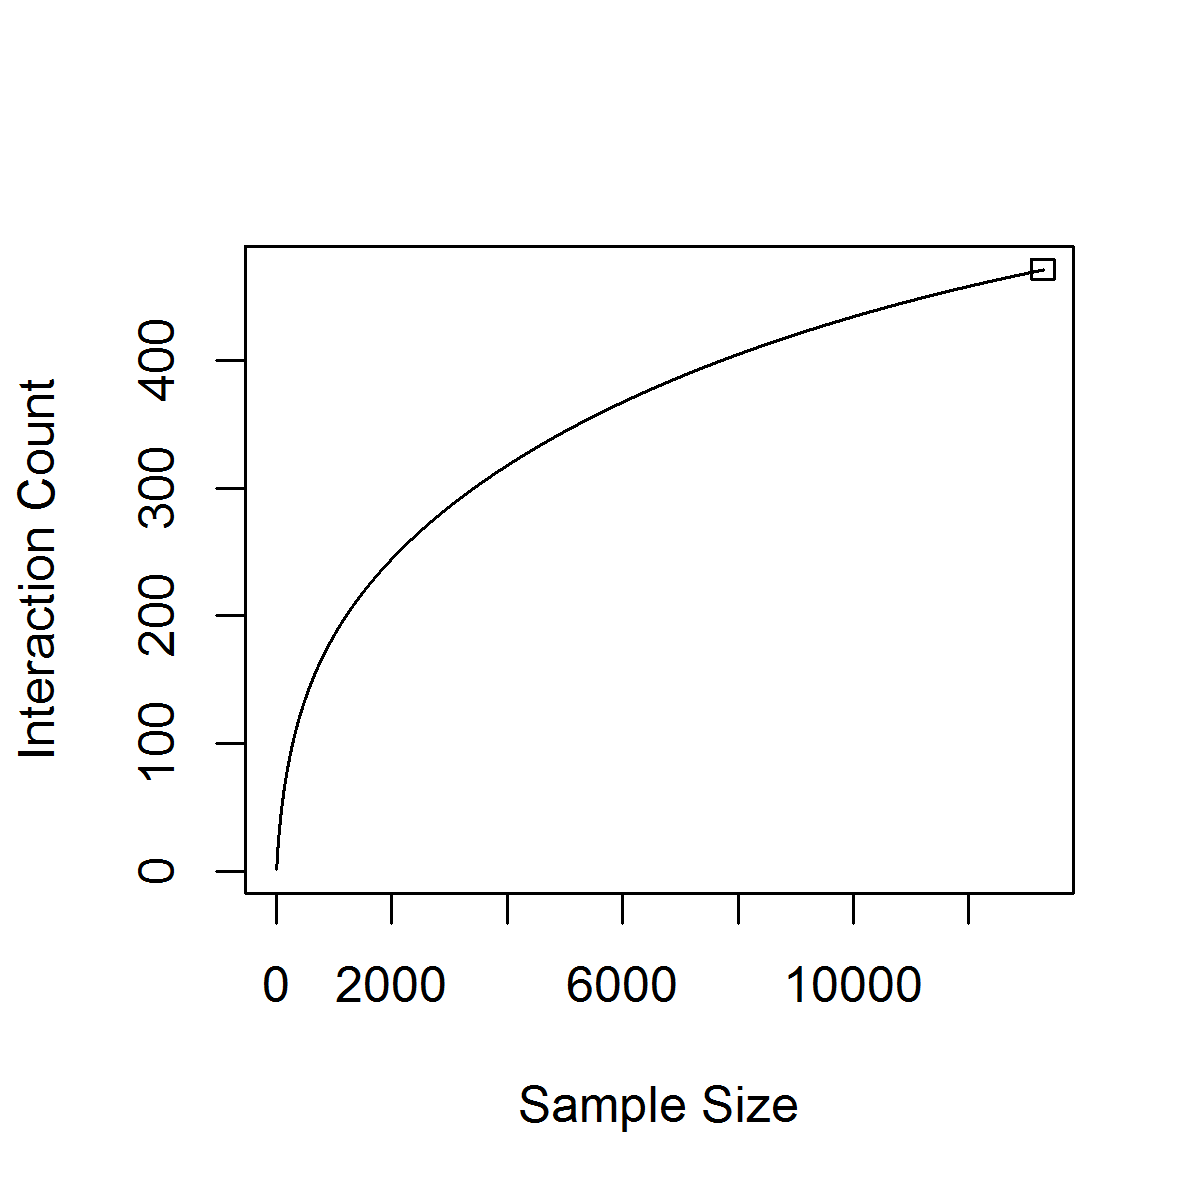
\includegraphics[width=0.7\textwidth]{../Figures/Rarefaction.png} 
\caption[]{\textbf{Figure S3.1} Rarefaction curve of sample size against accumulated interaction count. Although the accumulation curve has not plateaued, the rate of accumulation is low at large sample sizes.  }
\end{figure}

\subsection*{References for Appendix 3}

\begin{enumerate}
\item Chao, A. (1984). Nonparametric estimation of the number of classes in a population. Scand. J. Stat., 11, 265-270.
\item Gotelli, N.J. \& Colwell, R.K. (2010). Estimating species richness. In: Biological Diversity: Frontiers in Measurement and Assessment (eds. Magurran, AE \& McGill, BJ). Open University Press, pp. 416-422.
\item Jordano, P. (2016). Sampling networks of ecological interactions. Funct. Ecol., 30, 1883-1893.
\item Oksanen, J., Blanchet, F.G., Friendly, M., Kindt, R., Legendre, P., McGlinn, D. \emph{et al. }(2016). vegan: Community Ecology Package. R package version 2.4-0.  \url{https://CRAN.R-project.org/package=vegan}. 
\end{enumerate}

\section{Appendix S4: Supplementary results from random forest analyses}

The relative importance of individual plant traits in the analyses of the full data set are shown in Fig. S4.1. Although our models cannot predict our responses much better than random, it is notable that the same set of variables, in particular seed mass and tree height are consistently identified as important. This is despite tree height data only being available in 65\% of cases (see Appendix S1) – many of the remainder are lianas, for which ‘height’ is not meaningful. 



\begin{figure}[H]
\centering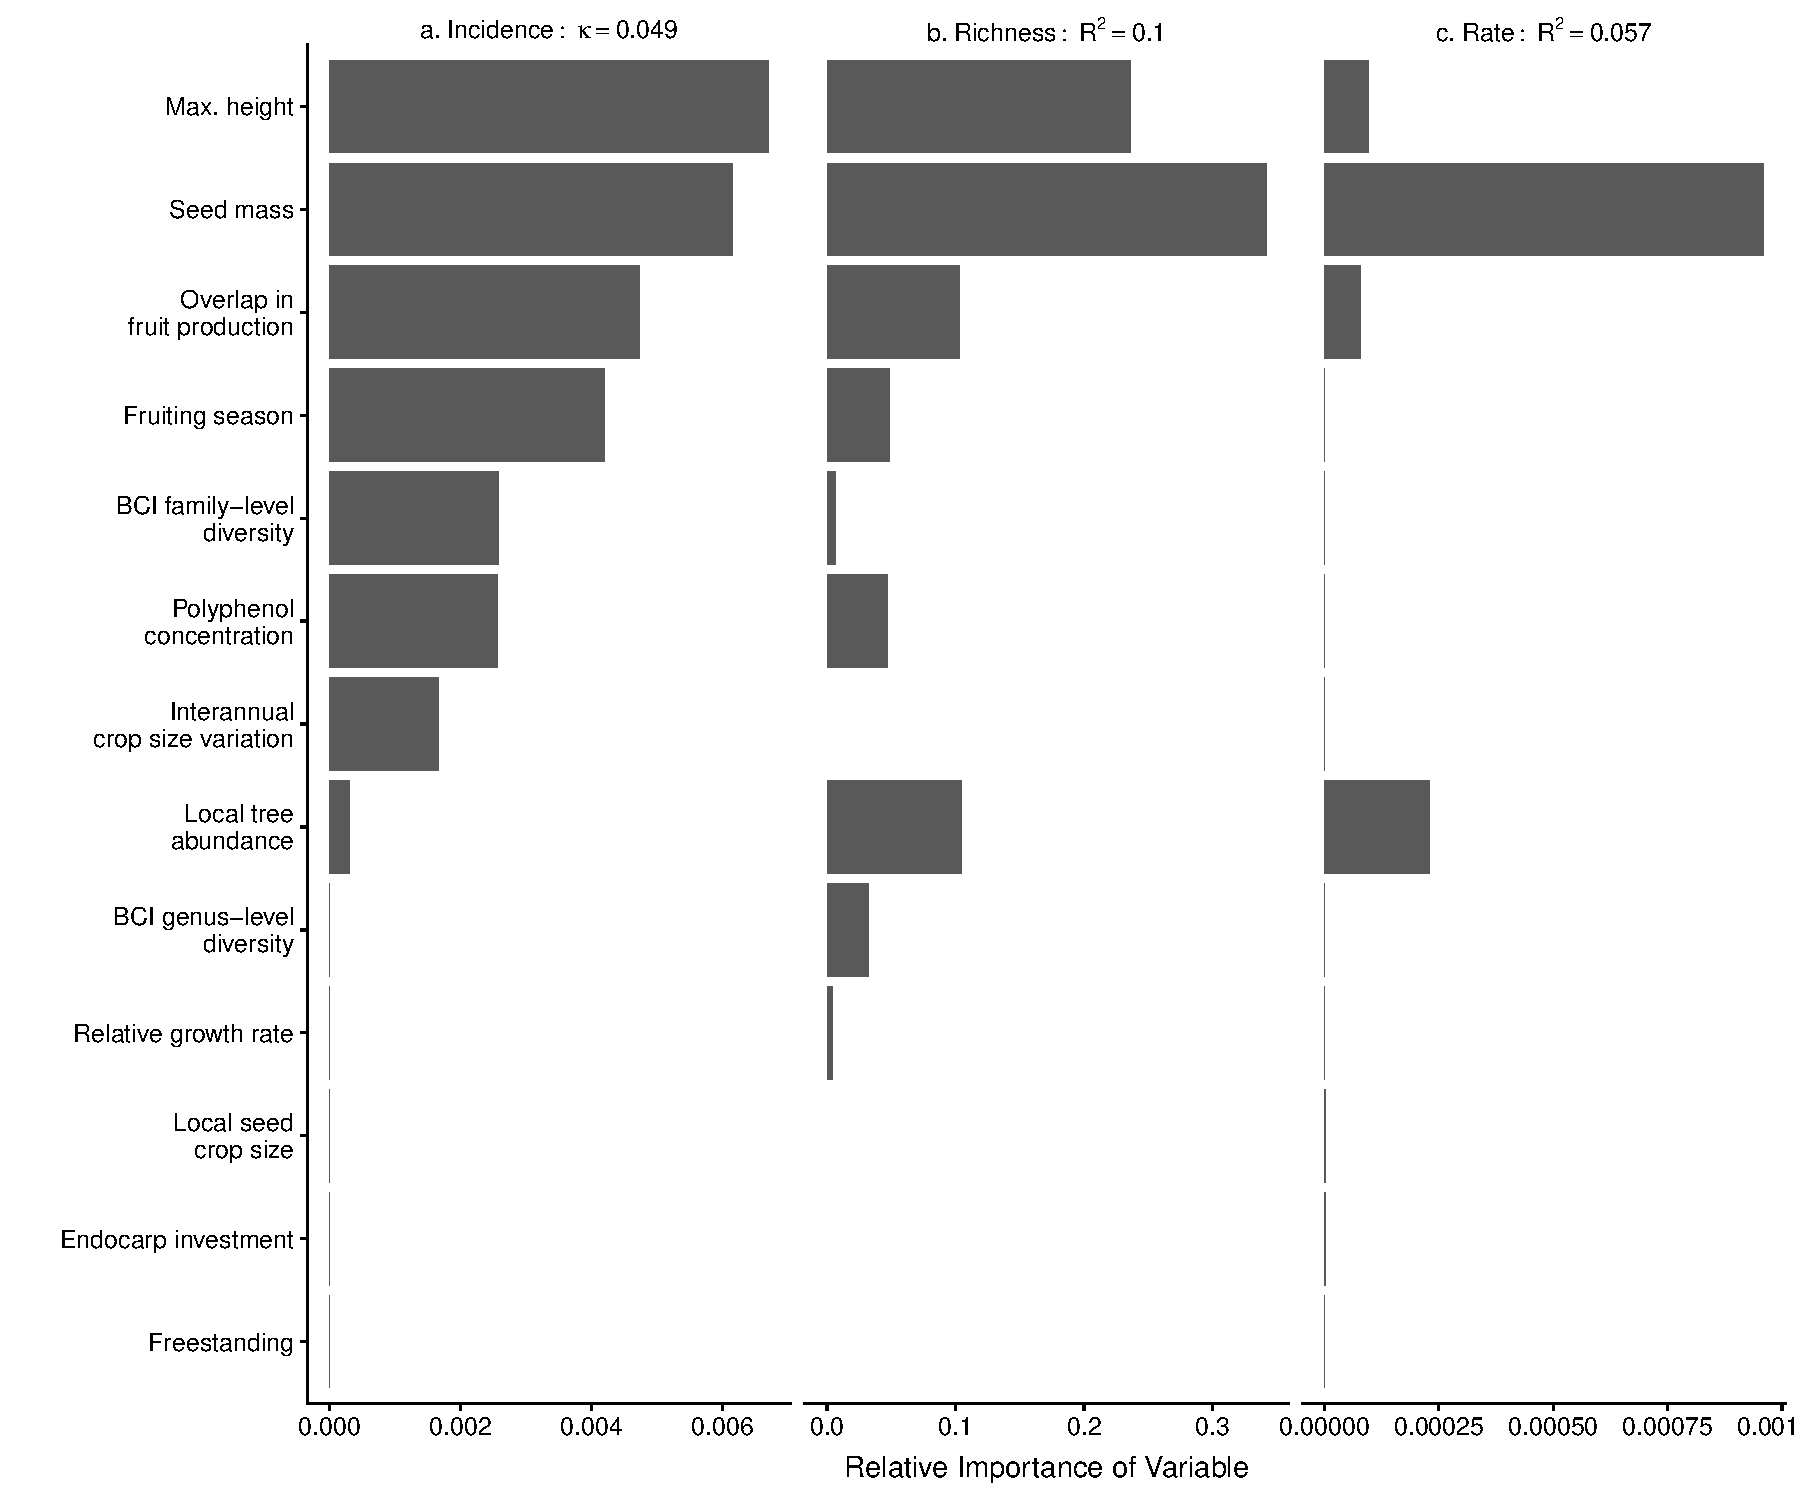
\includegraphics[width=\textwidth]{../Figures/VarImpPlot.pdf} 
\caption[]{\textbf{Figure S4.1.} Relative trait variable importance for our three response variables for the ‘well-sampled' dataset (including species with a minimum of 200 seeds/fruits). Variables are sorted according to their relative importance in explaining the incidence of seed predators. }
\end{figure}


An alternative approach to assessing how a model uses the information are partial dependence plots. These display how a model’s average predictions change as a predictor variable is changed, all else being equal. The partial dependence plots for seed mass and tree height are shown in Fig. S4.2, and generally match the patterns in Fig. 3 in the main text. 

\begin{figure}[H]
\centering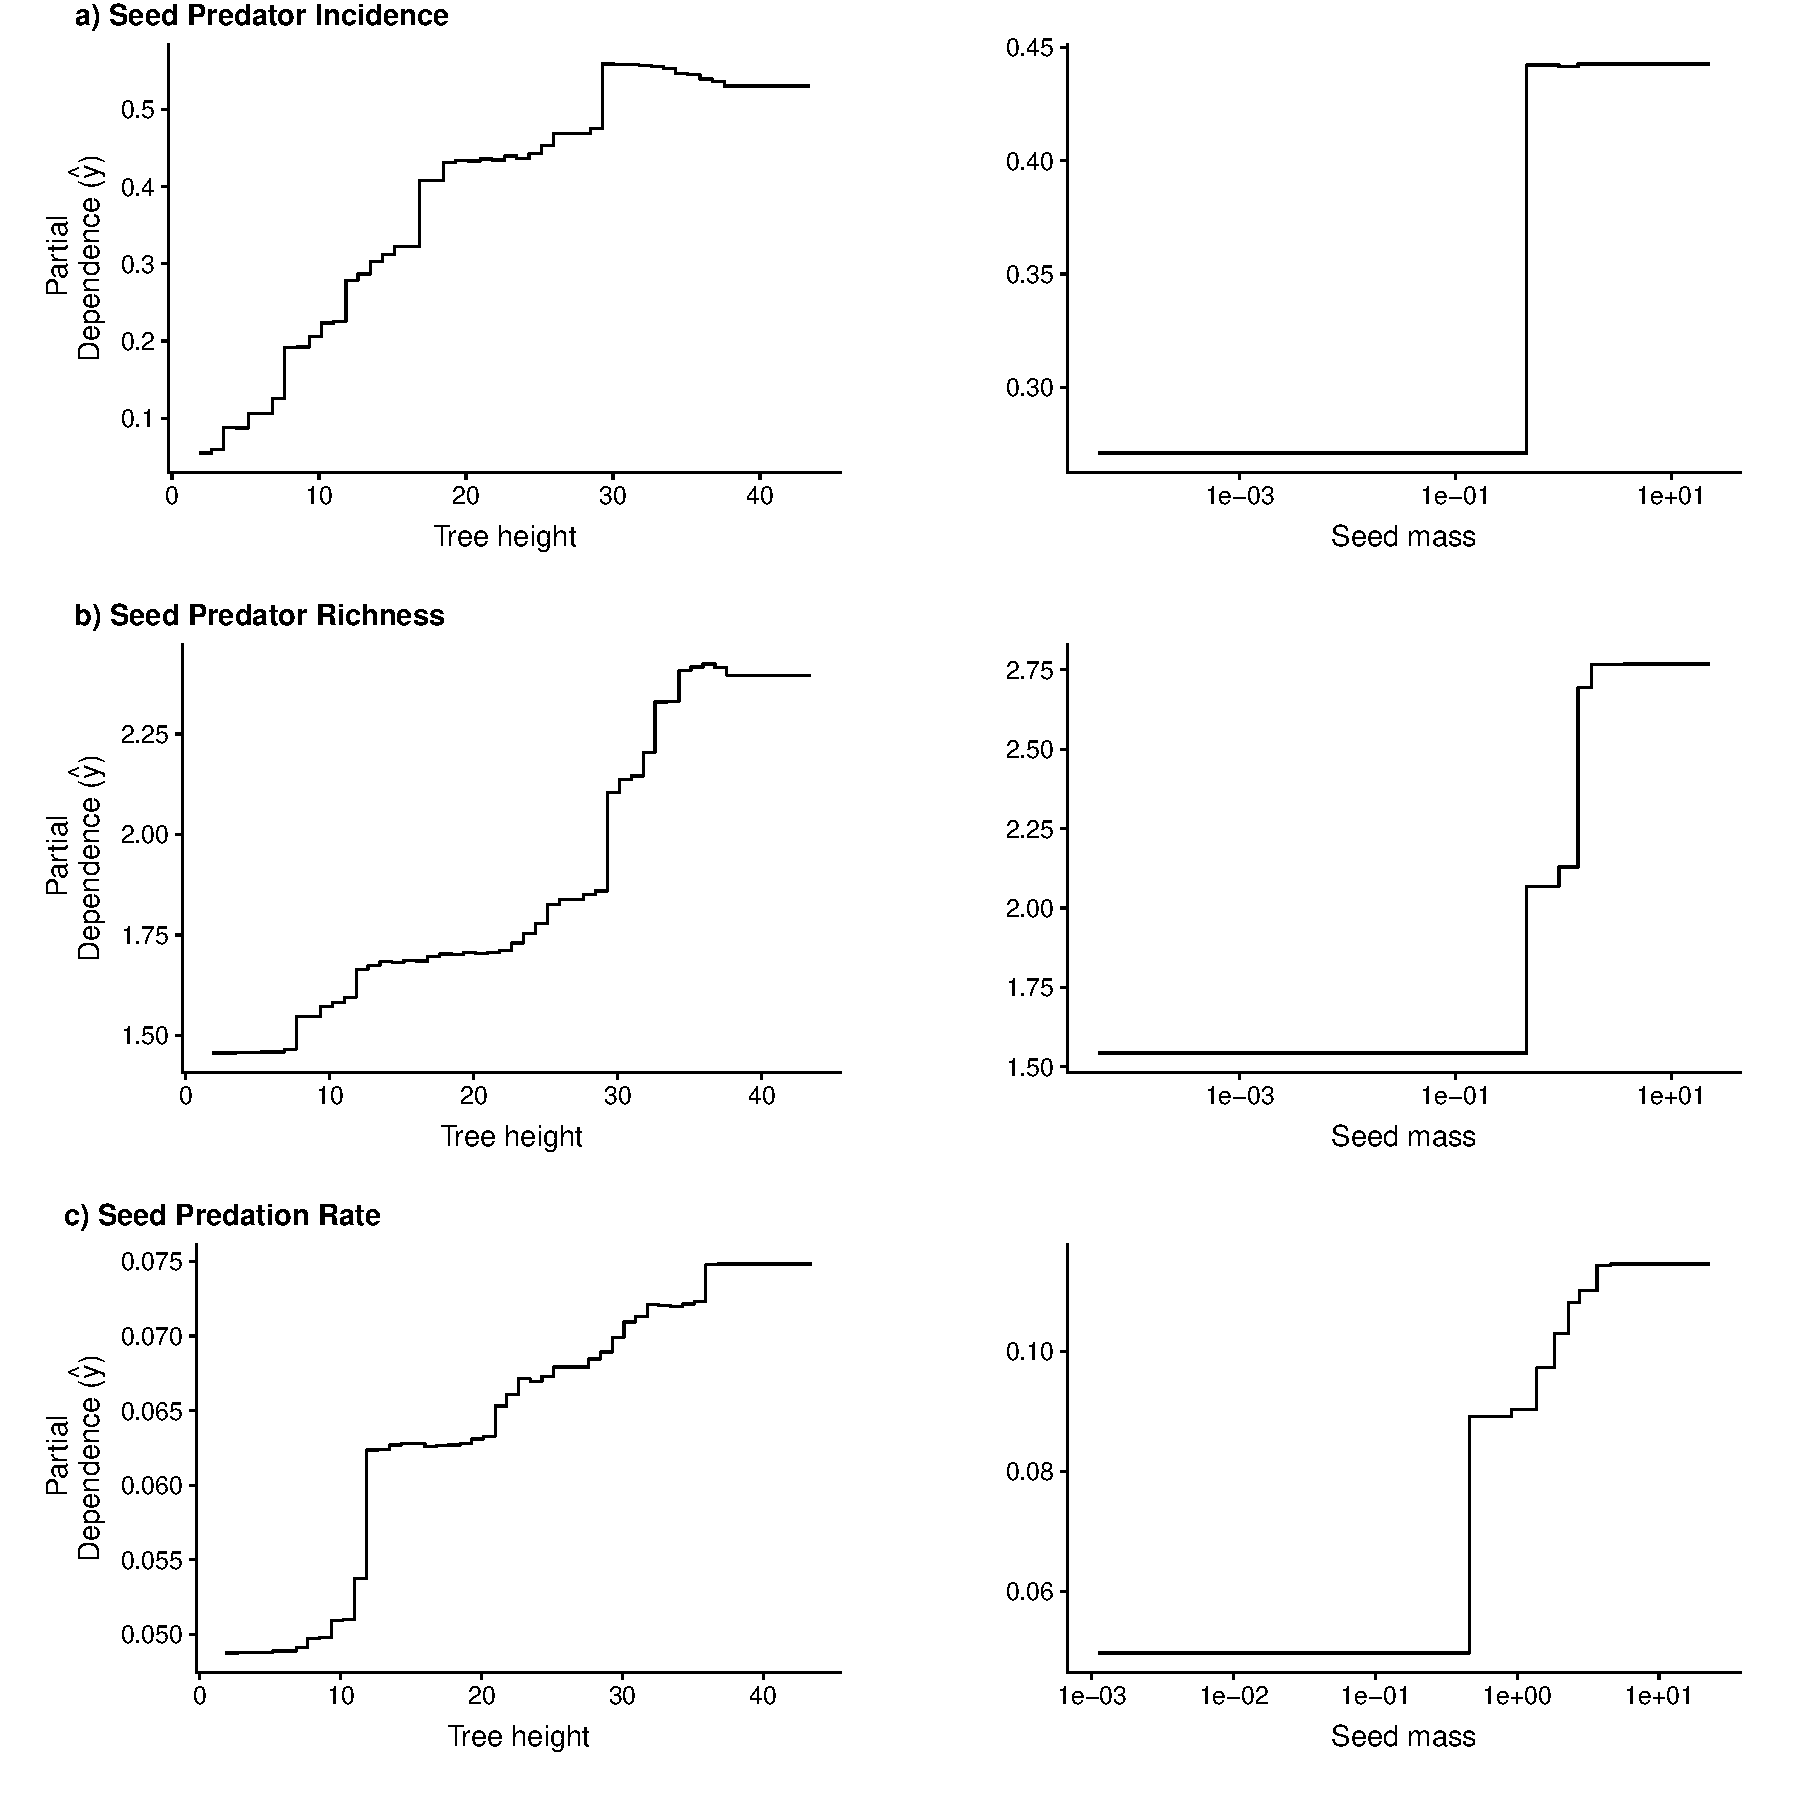
\includegraphics[width=0.7\textwidth]{../Figures/PartialDependencePlots.pdf} 
\caption[]{ \textbf{Figure S4.2}. Partial dependence plots for tree height and seed mass. These plots show how the predictions of our random forest models change in response to shifts in the values of a particular trait, against a representative background of other traits. There is a positive relationship between tree height and the susceptibility of species to seed predator attack and between seed mass and the susceptibility to seed predator attack. Note the logarithmic scale for seed mass.}
\end{figure}

To confirm that filtering of plants to include only well sampled species was not affecting the results, we also conducted a parallel analysis in which all plant species were included along with sample size as an additional predictor variable. Seed predator incidence could be predicted quite well, ($\kappa$ = 0.36), but by far the most important variable was the sample size (‘Total Units Collected’; Fig. S4.3). Species richness was predicted moderately well (pseudo-$R^2$ = 0.248), but this was again dominated by sample size. Species predation rate was poorly predicted on the full dataset (pseudo-$R^2$ = 0.0455), with sample size not driving rate.

\begin{figure}[H]
\centering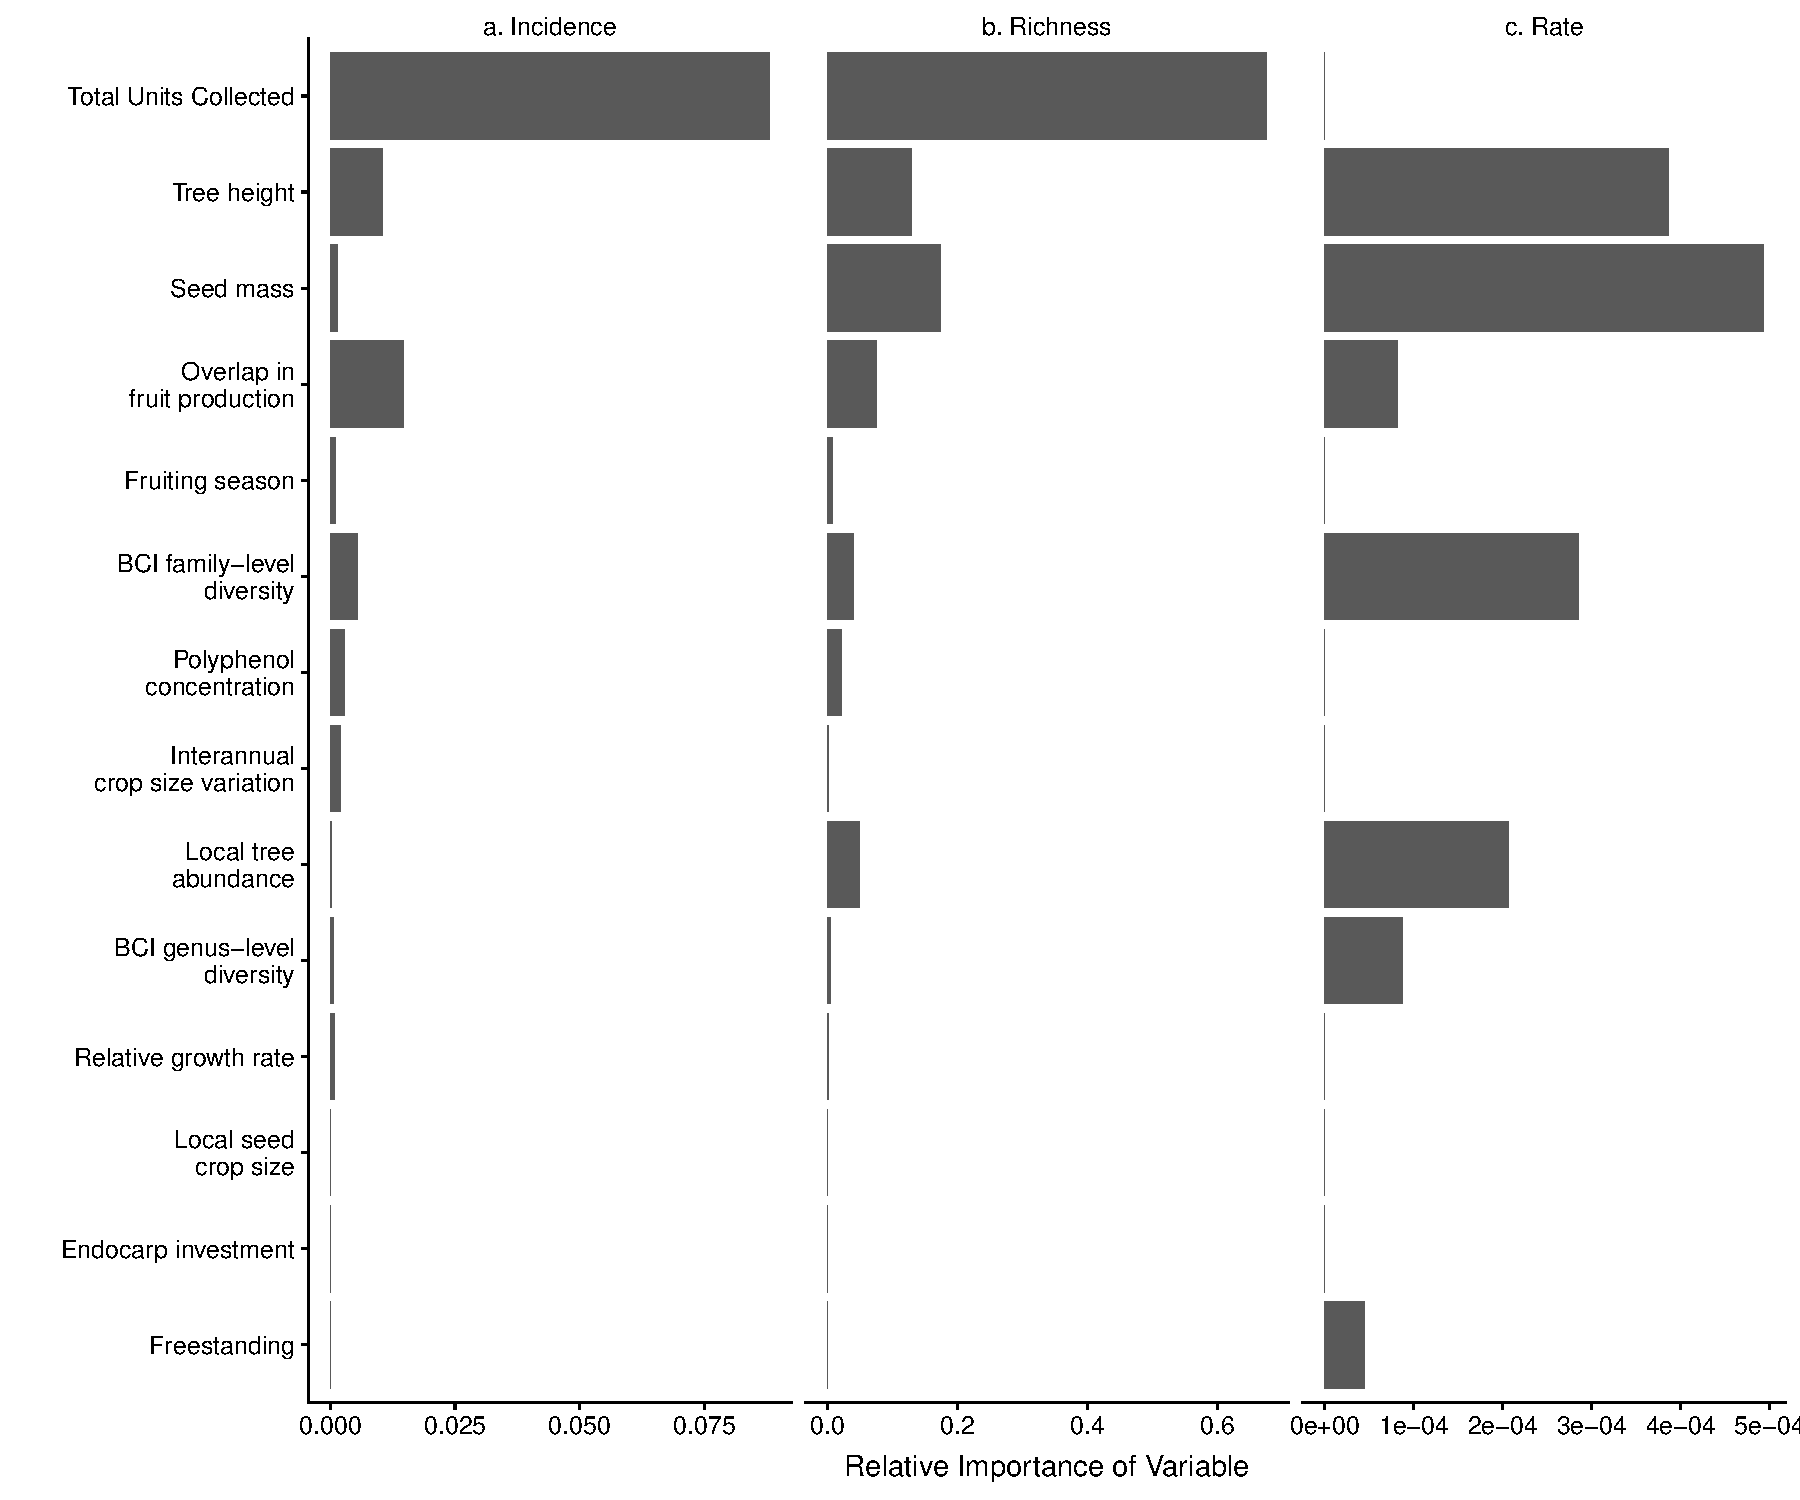
\includegraphics[width=\textwidth]{../Figures/VarImpPlotsall.pdf} 
\caption[]{\textbf{Figure S4.3}. Relative variable importance plots using the full dataset, which includes poorly sampled species. For both incidence and richness, total units collected was a driving feature.  }
\end{figure}




\newpage{}



\section{Table S1: List of sampled plant species} 


A list of the 478 plant species sampled for insect seed predators. For tree species occurring in the 50-ha forest dynamics plot, the nomenclature follows \url{http://conditdatacenter.org/taxonomy/BCI/BCIPlotFullTaxonomy.php} (accessed 14th December 2018). The nomenclature of remaining species follows \url{http://www.theplantlist.org} (accessed 8th January 2019). Code4 and Code6 are abbreviations of plant species names commonly used by researchers working on BCI. The column ‘Units collected’ shows the total number of seeds or fruits collected for insect rearing and the column ‘Phylogeny’ indicates whether or not (yes/no) the focal plant species was included in the phylogeny. Data on species-specific values of the 13 traits investigated in our analyses (Table 1 in the main text and Appendix S2) can be found in \url{https://github.com/jcdterry/BCI_Seed_Predator/} (to be made publicly available upon publication).


\footnotesize
\begin{longtable}{@{}llllll@{}}
\toprule
Species                                               & Family           & Code4  & Code6  & Units collected & Phylogeny \\* \midrule
\endfirsthead
\endhead
\bottomrule
\endfoot
\endlastfoot
\textit{Abuta racemosa}                               & Menispermaceae   & ABUR   & ABUTRA & 47              & Yes       \\
\textit{Acalypha macrostachya}                        & Euphorbiaceae    & ACA2   & ACALMA & 287             & Yes       \\
\textit{Acalypha diversifolia}                        & Euphorbiaceae    & ACAD   & ACALDI & 83              & Yes       \\
\textit{Acacia polyphylla}                            & Fabaceae         & ACAG   & NA     & 16              & Yes       \\
\textit{Acacia hayesii}                               & Fabaceae         & ACAH   & ACACHA & 196             & Yes       \\
\textit{Entadopsis polystachya}                       & Fabaceae         & ADEP   & ADE4PO & 183             & Yes       \\
\textit{Adelia triloba}                               & Euphorbiaceae    & ADET   & ADE1TR & 235             & Yes       \\
\textit{Aechmea setigera}                             & Bromeliaceae     & AECS   & NA     & 8               & No        \\
\textit{Aegiphila cephalophora}                       & Lamiaceae        & AEGC   & AEGICE & 477             & Yes       \\
\textit{Aegiphila panamensis}                         & Lamiaceae        & AEGP   & AEGIPA & 186             & Yes       \\
\textit{Alchornea costaricensis}                      & Euphorbiaceae    & ALCC   & ALCHCO & 323             & Yes       \\
\textit{Alibertia edulis}                             & Rubiaceae        & ALIE   & ALIBED & 166             & Yes       \\
\textit{Allamanda cathartica}                         & Apocynaceae      & ALLC   & ALLACA & 9               & Yes       \\
\textit{Allophylus psilospermus}                      & Sapindaceae      & ALLP   & ALLOPS & 1063            & Yes       \\
\textit{Alseis blackiana}                             & Rubiaceae        & ALSB   & ALSEBL & 5511            & Yes       \\
\textit{Amaioua corymbosa}                            & Rubiaceae        & AMAC   & AMAICO & 76              & Yes       \\
\textit{Amphilophium paniculatum}                     & Bignoniaceae     & AMPP   & AMPHPA & 362             & Yes       \\
\textit{Anacardium excelsum}                          & Anacardiaceae    & ANAE   & ANACEX & 396             & Yes       \\
\textit{Anaxagorea panamensis}                        & Annonaceae       & ANAP   & ANAXPA & 801             & Yes       \\
\textit{Andira inermis}                               & Fabaceae         & ANDI   & ANDIIN & 737             & Yes       \\
\textit{Annona glabra}                                & Annonaceae       & ANNG   & ANNOGL & 16              & Yes       \\
\textit{Annona hayesii}                               & Annonaceae       & ANNH   & ANNOHA & 46              & Yes       \\
\textit{Annona spraguei}                              & Annonaceae       & ANNS   & ANNOSP & 104             & Yes       \\
\textit{Anomospermum chloranthum\_isthmicola}         & Menispermaceae   & ANOC   & NA     & 89              & No        \\
\textit{Anthurium acutangulum}                        & Araceae          & ANTA   & NA     & 350             & No        \\
\textit{Anthurium brownii}                            & Araceae          & ANTB   & NA     & 2008            & No        \\
\textit{Anthurium clavigerum}                         & Araceae          & ANTC   & ANTHCL & 1484            & No        \\
\textit{Anthurium friedrichsthalii}                   & Araceae          & ANTF   & NA     & 133             & No        \\
\textit{Anthurium ochranthum}                         & Araceae          & ANTO   & NA     & 2               & No        \\
\textit{Anthodon panamense}                           & Celastraceae     & ANTP   & ANTHPA & 244             & Yes       \\
\textit{Apeiba membranacea}                           & Malvaceae        & APEM   & APEIME & 2070            & Yes       \\
\textit{Apeiba tibourbou}                             & Malvaceae        & APET   & APEITI & 711             & Yes       \\
\textit{Ardisia bartlettii}                           & Myrsinaceae      & ARDB   & ARDIBA & 183             & Yes       \\
\textit{Ardisia standleyana}                          & Myrsinaceae      & ARDF   & ARDIFE & 101             & Yes       \\
\textit{Ardisia guianensis}                           & Myrsinaceae      & ARDG   & ARDIGU & 136             & Yes       \\
\textit{Aristolochia gigantea}                        & Aristolochiaceae & ARI2   & ARISGI & 3               & Yes       \\
\textit{Aristolochia tonduzii}                        & Aristolochiaceae & ARIC   & ARISTO & 18              & Yes       \\
\textit{Fridericia candicans}                         & Bignoniaceae     & ARR1   & ARRACA & 127             & Yes       \\
\textit{Fridericia chica}                             & Bignoniaceae     & ARR2   & ARRACH & 138             & Yes       \\
\textit{Fridericia dichotoma}                         & Bignoniaceae     & ARR4   & NA     & 194             & Yes       \\
\textit{Fridericia florida}                           & Bignoniaceae     & ARRF   & ARRAFL & 253             & Yes       \\
\textit{Fridericia patellifera}                       & Bignoniaceae     & ARRP   & ARRAPA & 239             & Yes       \\
\textit{Fridericia schumanniana}                      & Bignoniaceae     & ARRV   & ARRAVE & 24              & Yes       \\
\textit{Aspidosperma desmanthum}                      & Apocynaceae      & ASPC   & ASPICR & 30              & Yes       \\
\textit{Astronium graveolens}                         & Anacardiaceae    & ASTG   & AST2GR & 1160            & Yes       \\
\textit{Astrocaryum standleyanum}                     & Arecaceae        & ASTS   & AST1ST & 283             & Yes       \\
\textit{Attalea rostrata}                             & Arecaceae        & ATTB   & SCH1ZO & 404             & Yes       \\
\textit{Bactris coloniata}                            & Arecaceae        & BAC1   & BACTC1 & 24              & Yes       \\
\textit{Bactris coloradensis}                         & Arecaceae        & BAC2   & BACTC2 & 803             & Yes       \\
\textit{Bactris maraja}                               & Arecaceae        & BAC5   & BACTM1 & 33              & Yes       \\
\textit{Bactris major}                                & Arecaceae        & BACM   & BACTMA & 183             & Yes       \\
\textit{Bauhinia purpurea}                            & Fabaceae         & BAU4   & NA     & 42              & Yes       \\
\textit{Bauhinia guianensis}                          & Fabaceae         & BAUG   & BAUHGU & 91              & Yes       \\
\textit{Bauhinia reflexa}                             & Fabaceae         & BAUR   & BAUHRE & 26              & Yes       \\
\textit{Beilschmiedia tovarensis}                     & Lauraceae        & BEIP   & BEILPE & 1986            & Yes       \\
\textit{Pochota quinata}                              & Bombacaceae      & BOMQ   & POCHQU & 59              & Yes       \\
\textit{Pachira sessilis}                             & Malvaceae        & BOMS   & POCHSE & 67              & Yes       \\
\textit{Brosimum alicastrum}                          & Moraceae         & BROA   & BROSAL & 562             & Yes       \\
\textit{Bucida buceras}                               & Combretaceae     & BUCB   & BUCIBU & 18              & No        \\
\textit{Buchenavia tetraphylla}                       & Combretaceae     & BUCT   & BUCHCA & 163             & No        \\
\textit{Bunchosia nitida}                             & Malpighiaceae    & BUNC   & BUNCCO & 46              & No        \\
\textit{Bursera simaruba}                             & Burseraceae      & BURS   & BURSSI & 2023            & No        \\
\textit{Byrsonima crassifolia}                        & Malpighiaceae    & BYRC   & BYRSCR & 74              & No        \\
\textit{Canavalia gladiata}                           & Fabaceae         & CAGL   & NA     & 15              & No        \\
\textit{Callichlamys latifolia}                       & Bignoniaceae     & CAL1   & CALLLA & 473             & Yes       \\
\textit{Calophyllum longifolium}                      & Clusiaceae       & CAL2   & CALOLO & 996             & Yes       \\
\textit{Calathea inocephala}                          & Marantaceae      & CALI   & NA     & 54              & No        \\
\textit{Canavalia dictyota}                           & Fabaceae         & CAND   & NA     & 22              & No        \\
\textit{Capparidastrum frondosa}                      & Capparaceae      & CAPF   & CAPPFR & 144             & Yes       \\
\textit{Vasconcellea cauliflora}                      & Caricaceae       & CARC   & CARICA & 6               & No        \\
\textit{Casearia aculeata}                            & Salicaceae       & CAS1   & CASEAC & 121             & Yes       \\
\textit{Casearia arborea}                             & Salicaceae       & CAS2   & CASEAR & 1475            & Yes       \\
\textit{Cassipourea elliptica}                        & Rhizophoraceae   & CAS3   & CASSEL & 301             & Yes       \\
\textit{Castilla elastica}                            & Moraceae         & CAS4   & CASTEL & 7               & No        \\
\textit{Casearia commersoniana}                       & Salicaceae       & CASC   & CASECO & 608             & Yes       \\
\textit{Casearia guianensis}                          & Salicaceae       & CASG   & CASEGU & 103             & Yes       \\
\textit{Cavanillesia platanifolia}                    & Malvaceae        & CAVP   & CAVAPL & 294             & Yes       \\
\textit{Cayaponia granatensis}                        & Cucurbitaceae    & CAYG   & CAYAGR & 10              & Yes       \\
\textit{Cecropia insignis}                            & Urticaceae       & CECI   & CECRIN & 185             & Yes       \\
\textit{Cecropia obtusifolia}                         & Urticaceae       & CECO   & CECROB & 196             & Yes       \\
\textit{Cecropia peltata}                             & Urticaceae       & CECP   & CECRPE & 139             & Yes       \\
\textit{Cedrela odorata}                              & Meliaceae        & CEDO   & CEDROD & 104             & Yes       \\
\textit{Ceiba pentandra}                              & Malvaceae        & CEIP   & CEIBPE & 580             & Yes       \\
\textit{Celtis iguanaea}                              & Cannabaceae      & CELI   & CELTIG & 283             & Yes       \\
\textit{Celtis schippii}                              & Cannabaceae      & CELS   & CELTSC & 360             & Yes       \\
\textit{Tanaecium tetragonolobum}                     & Bignoniaceae     & CERT   & CERATE & 452             & Yes       \\
\textit{Chamaedorea tepejilote}                       & Arecaceae        & CHAW   & CHA1TE & 603             & Yes       \\
\textit{Chomelia psilocarpa}                          & Rubiaceae        & CHOP   & CHOMPS & 8               & Yes       \\
\textit{Chondrodendron tomentosum}                    & Menispermaceae   & CHOT   & CHONTO & 81              & Yes       \\
\textit{Chrysophyllum argenteum}                      & Sapotaceae       & CHRA   & CHR2AR & 397             & Yes       \\
\textit{Chrysophyllum cainito}                        & Sapotaceae       & CHRC   & CHR2CA & 410             & Yes       \\
\textit{Cissus erosa}                                 & Vitaceae         & CISE   & CISSER & 472             & Yes       \\
\textit{Cissus verticillata}                          & Vitaceae         & CISS   & CISSSI & 64              & Yes       \\
\textit{Clitoria javitensis}                          & Fabaceae         & CLIJ   & CLITJA & 36              & Yes       \\
\textit{Clidemia octona}                              & Melastomataceae  & CLIO   & CLIDOC & 122             & Yes       \\
\textit{Clidemia septuplinervia}                      & Melastomataceae  & CLIS   & CLIDSE & 153             & Yes       \\
\textit{Clusia minor}                                 & Clusiaceae       & CLUM   & NA     & 4               & No        \\
\textit{Clusia peninsularis}                          & Clusiaceae       & CLUP   & NA     & 113             & No        \\
\textit{Clusia uvitana}                               & Clusiaceae       & CLUU   & NA     & 444             & No        \\
\textit{Cnestidium rufescens}                         & Connaraceae      & CNER   & CNESRU & 1121            & Yes       \\
\textit{Coccoloba aculeata}                           & Polygonaceae     & COC2   & COCCA2 & 145             & Yes       \\
\textit{Coccoloba coronata}                           & Polygonaceae     & COCC   & COCCCO & 1420            & Yes       \\
\textit{Coccoloba manzinellensis}                     & Polygonaceae     & COCM   & COCCMA & 2908            & Yes       \\
\textit{Coccoloba excelsa}                            & Polygonaceae     & COCP   & COCCP1 & 671             & Yes       \\
\textit{Cochlospermum vitifolium}                     & Bixaceae         & COCV   & COCHVI & 1               & No        \\
\textit{Colubrina glandulosa}                         & Rhamnaceae       & COLG   & COLUGL & 215             & No        \\
\textit{Combretum cacoucia}                           & Combretaceae     & COMC   & COMBCA & 45              & Yes       \\
\textit{Combretum decandrum}                          & Combretaceae     & COMD   & COMBDE & 618             & Yes       \\
\textit{Combretum fruticosum}                         & Combretaceae     & COMF   & COMBFR & 719             & Yes       \\
\textit{Combretum laxum}                              & Combretaceae     & COML   & COMBLA & 348             & Yes       \\
\textit{Conostegia cinnamomea}                        & Melastomataceae  & CONC   & CONOCI & 335             & Yes       \\
\textit{Connarus panamensis}                          & Connaraceae      & CONP   & CONNPA & 559             & Yes       \\
\textit{Connarus turczaninowii}                       & Connaraceae      & CONT   & CONNTU & 434             & Yes       \\
\textit{Copaifera aromatica}                          & Fabaceae         & COPA   & COPAAR & 23              & No        \\
\textit{Cordia alliodora}                             & Cordiaceae       & CORA   & CORDAL & 2630            & Yes       \\
\textit{Cordia bicolor}                               & Cordiaceae       & CORB   & CORDBI & 1684            & Yes       \\
\textit{Cordia lasiocalyx}                            & Cordiaceae       & CORL   & CORDLA & 335             & Yes       \\
\textit{Cordia panamensis}                            & Boraginaceae     & CORP   & CORDPA & 280             & Yes       \\
\textit{Cosmibuena grandiflora}                       & Rubiaceae        & COSS   & COSMGR & 4               & No        \\
\textit{Coussarea curvigemmia}                        & Rubiaceae        & COUC   & COU2CU & 2273            & Yes       \\
\textit{Coutarea hexandra}                            & Rubiaceae        & COUH   & COUTHE & 31              & Yes       \\
\textit{Couratari guianensis}                         & Lecythidaceae    & COUP   & COURPA & 5               & No        \\
\textit{Mosannona garwoodii}                          & Annonaceae       & CRES   & MALMSP & 99              & Yes       \\
\textit{Croton billbergianus}                         & Euphorbiaceae    & CROB   & CROTBI & 803             & Yes       \\
\textit{Cuervea kappleriana}                          & Celastraceae     & CUEK   & CUERKA & 41              & Yes       \\
\textit{Cupania latifolia}                            & Sapindaceae      & CUPL   & CUPALA & 507             & Yes       \\
\textit{Cupania rufescens}                            & Sapindaceae      & CUPR   & CUPARU & 46              & Yes       \\
\textit{Cupania seemannii}                            & Sapindaceae      & CUPS   & CUPASY & 746             & Yes       \\
\textit{Bignonia aequinoctialis}                      & Bignoniaceae     & CYDA   & CYDIAE & 235             & Yes       \\
\textit{Solanum circinatum}                           & Solanaceae       & CYPH   & CYPHHA & 2               & Yes       \\
\textit{Dalechampia dioscoreifolia}                   & Euphorbiaceae    & DALD   & DALEDI & 12              & Yes       \\
\textit{Davilla nitida}                               & Dilleniaceae     & DAVN   & DAVINI & 983             & Yes       \\
\textit{Dendropanax arboreus}                         & Araliaceae       & DENA   & DENDAR & 2239            & Yes       \\
\textit{Desmodium axillare}                           & Fabaceae         & DESA   & DESMAX & 206             & Yes       \\
\textit{Desmodium incanum}                            & Fabaceae         & DESC   & NA     & 32              & Yes       \\
\textit{Desmoncus orthacanthos}                       & Arecaceae        & DESI   & DES1OR & 514             & Yes       \\
\textit{Desmopsis panamensis}                         & Annonaceae       & DESP   & DES2PA & 298             & Yes       \\
\textit{Dichapetalum gentryi}                         & Dichapetalaceae  & DICG   & NA     & 3               & No        \\
\textit{Diospyros artanthifolia}                      & Ebenaceae        & DIO2   & DIO2AR & 11              & Yes       \\
\textit{Dioclea wilsonii}                             & Fabaceae         & DIOW   & DIOCWI & 85              & Yes       \\
\textit{Dipteryx oleifera}                            & Fabaceae         & DIPP   & DIPTPA & 607             & Yes       \\
\textit{Doliocarpus major}                            & Dilleniaceae     & DOL1   & DOLIMA & 940             & Yes       \\
\textit{Doliocarpus multiflorus}                      & Dilleniaceae     & DOL2   & DOLIMU & 669             & Yes       \\
\textit{Doliocarpus dentatus}                         & Dilleniaceae     & DOLD   & DOLIDE & 2               & Yes       \\
\textit{Doliocarpus olivaceus}                        & Dilleniaceae     & DOLO   & DOLIOL & 842             & Yes       \\
\textit{Drypetes standleyi}                           & Putranjivaceae   & DRYS   & DRYPST & 289             & Yes       \\
\textit{Enterolobium cyclocarpum}                     & Fabaceae         & ENTC   & ENTECY & 19              & Yes       \\
\textit{Entada rhedii}                                & Fabaceae         & ENTM   & ENTAMO & 76              & Yes       \\
\textit{Enterolobium schomburgkii}                    & Fabaceae         & ENTS   & ENTESC & 180             & Yes       \\
\textit{Epiphyllum phyllanthus var.rubrocoronatum} & Cactaceae        & EPPR   & NA     & 3               & No        \\
\textit{Erythrina costaricensis}                      & Fabaceae         & ERYC   & ERY1CO & 2               & Yes       \\
\textit{Eugenia coloradoensis}                        & Myrtaceae        & EUGC   & EUGECO & 464             & Yes       \\
\textit{Eugenia galalonensis}                         & Myrtaceae        & EUGG   & EUGEGA & 84              & Yes       \\
\textit{Eugenia nesiotica}                            & Myrtaceae        & EUGN   & EUGENE & 278             & Yes       \\
\textit{Eugenia oerstediana}                          & Myrtaceae        & EUGO   & EUGEOE & 152             & Yes       \\
\textit{Eugenia venezuelensis}                        & Myrtaceae        & EUGV   & EUGEVE & 508             & Yes       \\
\textit{Faramea luteovirens}                          & Rubiaceae        & FARL   & FARALU & 146             & Yes       \\
\textit{Faramea occidentalis}                         & Rubiaceae        & FARO   & FARAOC & 3085            & Yes       \\
\textit{Fevillea cordifolia}                          & Cucurbitaceae    & FEVC   & FEVICO & 36              & Yes       \\
\textit{Ficus colubrinae}                             & Moraceae         & FIC1   & FICUC1 & 273             & Yes       \\
\textit{Ficus costaricana}                            & Moraceae         & FIC2   & FICUC2 & 17              & Yes       \\
\textit{Ficus citrifolia}                             & Moraceae         & FICI   & FICUCI & 1497            & Yes       \\
\textit{Ficus insipida}                               & Moraceae         & FIIN   & FICUIN & 519             & Yes       \\
\textit{Ficus maxima}                                 & Moraceae         & FIMA   & FICUMA & 56              & Yes       \\
\textit{Ficus nymphaeifolia}                          & Moraceae         & FINY   & FICUNY & 126             & Yes       \\
\textit{Ficus obtusifolia}                            & Moraceae         & FIOB   & FICUOB & 107             & Yes       \\
\textit{Ficus pertusa}                                & Moraceae         & FIP2   & FICUPE & 861             & Yes       \\
\textit{Ficus paraensis}                              & Moraceae         & FIPA   & FICUPA & 32              & Yes       \\
\textit{Ficus popenoei}                               & Moraceae         & FIPO   & FICUPO & 269             & Yes       \\
\textit{Fischeria blepharopetala}                     & Apocynaceae      & FISF   & FISCBL & 5               & No        \\
\textit{Ficus tonduzii}                               & Moraceae         & FITO   & FICUTO & 25              & Yes       \\
\textit{Ficus trigonata}                              & Moraceae         & FITR   & FICUTR & 219             & Yes       \\
\textit{Ficus yoponensis}                             & Moraceae         & FIYO   & FICUYO & 64              & Yes       \\
\textit{Forsteronia acouci}                           & Apocynaceae      & FORV   & FORSVI & 129             & Yes       \\
\textit{Geonoma congesta}                             & Arecaceae        & GEC2   & GEONCO & 120             & No        \\
\textit{Genipa americana}                             & Rubiaceae        & GENA   & GENIAM & 59              & Yes       \\
\textit{Geonoma cuneata\_procumbens}                  & Arecaceae        & GEOC   & GEONCU & 144             & No        \\
\textit{Geophila repens}                              & Rubiaceae        & GEOR   & NA     & 21              & No        \\
\textit{Gnetum leyboldii}                             & Gnetaceae        & GNEL   & GNETLE & 140             & Yes       \\
\textit{Gouania colombiana}                           & Rhamnaceae       & GOUC   & GOUACO & 62              & Yes       \\
\textit{Gouania lupuloides}                           & Rhamnaceae       & GOUL   & GOUALU & 723             & Yes       \\
\textit{Gouania polygama}                             & Rhamnaceae       & GOUP   & GOUAPO & 135             & Yes       \\
\textit{Guarea grandifolia}                           & Meliaceae        & GUA1   & GUARGR & 636             & Yes       \\
\textit{Guarea guidonia}                              & Meliaceae        & GUA2   & GUARGU & 443             & Yes       \\
\textit{Guatteria amplifolia}                         & Annonaceae       & GUAA   & GUATAM & 266             & Yes       \\
\textit{Guatteria lucens}                             & Annonaceae       & GUAD   & GUATDU & 778             & Yes       \\
\textit{Guapira standleyana}                          & Nyctaginaceae    & GUAS   & GUAPST & 1785            & Yes       \\
\textit{Guazuma ulmifolia}                            & Malvaceae        & GUAU   & GUAZUL & 320             & Yes       \\
\textit{Guettarda foliacea}                           & Rubiaceae        & GUEF   & GUETFO & 527             & Yes       \\
\textit{Gustavia superba}                             & Lecythidaceae    & GUSS   & GUSTSU & 602             & Yes       \\
\textit{Hamelia axillaris}                            & Rubiaceae        & HAM1   & HAMEAX & 96              & Yes       \\
\textit{Hamelia patens}                               & Rubiaceae        & HAMP   & HAMEPA & 38              & Yes       \\
\textit{Hasseltia floribunda}                         & Salicaceae       & HASF   & HASSFL & 331             & Yes       \\
\textit{Clusia flavida}                               & Clusiaceae       & HAVF   & HAVEFL & 190             & No        \\
\textit{Heisteria acuminata}                          & Erythropalaceae  & HEIA   & HEISAC & 429             & Yes       \\
\textit{Heisteria concinna}                           & Erythropalaceae  & HEIC   & HEISCO & 879             & Yes       \\
\textit{Heliconia platystachys}                       & Heliconiaceae    & HEL1   & NA     & 55              & No        \\
\textit{Henriettea succosa}                           & Melastomataceae  & HENS   & HENRSU & 68              & No        \\
\textit{Herrania purpurea}                            & Malvaceae        & HERP   & HERRPU & 35              & Yes       \\
\textit{Heteropteris laurifolia}                      & Malpighiaceae    & HETL   & HETELA & 353             & Yes       \\
\textit{Hippocratea volubilis}                        & Celastraceae     & HIPV   & HIPPVO & 575             & Yes       \\
\textit{Hiraea reclinata}                             & Malpighiaceae    & HIR1   & HIRARE & 650             & Yes       \\
\textit{Hiraea fagifolia}                             & Malpighiaceae    & HIR3   & HIRAF1 & 22              & Yes       \\
\textit{Hirtella americana}                           & Chrysobalanaceae & HIRA   & HIRTAM & 73              & Yes       \\
\textit{Hiraea faginea}                               & Malpighiaceae    & HIRF   & HIRAFA & 184             & Yes       \\
\textit{Hiraea grandifolia}                           & Malpighiaceae    & HIRG   & HIRAGR & 152             & Yes       \\
\textit{Hiraea smilacina}                             & Malpighiaceae    & HIRQ   & HIRAQU & 152             & Yes       \\
\textit{Hirtella triandra}                            & Chrysobalanaceae & HIRT   & HIRTTR & 181             & Yes       \\
\textit{Hura crepitans}                               & Euphorbiaceae    & HURC   & HURACR & 23              & Yes       \\
\textit{Pombalia prunifolia}                          & Violaceae        & HYBP   & HYBAPR & 694             & Yes       \\
\textit{Hieronyma alchorneoides}                      & Euphorbiaceae    & HYEL   & HYERAL & 7480            & Yes       \\
\textit{Hylenaea praecelsa}                           & Celastraceae     & HYLP   & HYLEPR & 466             & Yes       \\
\textit{Hymenaea courbaril}                           & Fabaceae         & HYMC   & HYMECO & 89              & No        \\
\textit{Inga acuminata}                               & Fabaceae         & INA1   & INGAS1 & 32              & Yes       \\
\textit{Inga cocleensis}                              & Fabaceae         & INCO   & INGACO & 42              & Yes       \\
\textit{Inga laurina}                                 & Fabaceae         & INFA   & INGARU & 505             & Yes       \\
\textit{Inga alba}                                    & Fabaceae         & INGAAL & INGAAL & 2               & Yes       \\
\textit{Inga goldmanii}                               & Fabaceae         & INGO   & INGAGO & 11              & Yes       \\
\textit{Inga mucuna}                                  & Fabaceae         & INM1   & INGAM1 & 19              & Yes       \\
\textit{Inga multijuga}                               & Fabaceae         & INM2   & INGAM2 & 73              & Yes       \\
\textit{Inga marginata}                               & Fabaceae         & INMA   & INGAMA & 168             & Yes       \\
\textit{Inga oersterdiana}                            & Fabaceae         & INMI   & INGAMI & 24              & Yes       \\
\textit{Inga pauciflora}                              & Fabaceae         & INPA   & INGAPA & 120             & Yes       \\
\textit{Inga pezizifera}                              & Fabaceae         & INPE   & INGAPE & 35              & Yes       \\
\textit{Inga punctata}                                & Fabaceae         & INPU   & INGAPU & 315             & Yes       \\
\textit{Inga nobilis}                                 & Fabaceae         & INQU   & INGAQU & 13              & Yes       \\
\textit{Inga ruiziana}                                & Fabaceae         & INRU   & INGARU & 17              & Yes       \\
\textit{Inga sapindoides}                             & Fabaceae         & INSA   & INGASA & 305             & Yes       \\
\textit{Inga thibaudiana}                             & Fabaceae         & INTH   & INGATH & 39              & Yes       \\
\textit{Inga umbellifera}                             & Fabaceae         & INUM   & INGAUM & 39              & Yes       \\
\textit{Jacaranda copaia}                             & Bignoniaceae     & JACC   & JAC1CO & 626             & Yes       \\
\textit{Jacaratia spinosa}                            & Caricaceae       & JACS   & JAC2SP & 2               & No        \\
\textit{Lacistema aggregatum}                         & Lacistemataceae  & LACA   & LACIAG & 1019            & Yes       \\
\textit{Lacmellea panamensis}                         & Apocynaceae      & LACP   & LACMPA & 783             & Yes       \\
\textit{Laetia procera}                               & Salicaceae       & LAEP   & LAETPR & 78              & Yes       \\
\textit{Laetia thamnia}                               & Salicaceae       & LAET   & LAETTH & 232             & Yes       \\
\textit{Lafoensia punicifolia}                        & Lythraceae       & LAFP   & LAFOPU & 312             & Yes       \\
\textit{Lagerstroemia speciosa}                       & Lythraceae       & LAGS   & LAGESP & 61              & No        \\
\textit{Lasiacis maculata}                            & Poaceae          & LASS   & NA     & 690             & No        \\
\textit{Leandra dichotoma}                            & Melastomataceae  & LEAD   & LEANDI & 842             & Yes       \\
\textit{Licania hypoleuca}                            & Chrysobalanaceae & LICH   & LICAHY & 2               & Yes       \\
\textit{Licania platypus}                             & Chrysobalanaceae & LICP   & LICAPL & 627             & Yes       \\
\textit{Lindackeria laurina}                          & Achariaceae      & LINL   & LINDLA & 902             & Yes       \\
\textit{Lonchocarpus luteomaculatus}                  & Fabaceae         & LON1   & NA     & 358             & Yes       \\
\textit{Lonchocarpus ferrugineus}                     & Fabaceae         & LONF   & LONCFE & 77              & Yes       \\
\textit{Lonchocarpus heptaphyllus}                    & Fabaceae         & LONL   & LONCLA & 654             & Yes       \\
\textit{Lozania pittieri}                             & Lacistemataceae  & LOZP   & LOZAPI & 30              & Yes       \\
\textit{Luehea seemannii}                             & Malvaceae        & LUE1   & LUEHSE & 778             & Yes       \\
\textit{Lycianthes maxonii}                           & Solanaceae       & LYCM   & LYCIMA & 48              & Yes       \\
\textit{Mabea occidentalis}                           & Euphorbiaceae    & MABO   & MABEOC & 750             & No        \\
\textit{Machaerium microphyllum}                      & Fabaceae         & MAC1   & MACHM1 & 142             & Yes       \\
\textit{Machaerium milleflorum}                       & Fabaceae         & MAC2   & MACHM2 & 443             & Yes       \\
\textit{Machaerium arboreum}                          & Fabaceae         & MACA   & MACHAR & 279             & Yes       \\
\textit{Macrocnemum roseum}                           & Rubiaceae        & MACG   & MACRGL & 1741            & Yes       \\
\textit{Machaerium kegelii}                           & Fabaceae         & MACK   & MACHKE & 295             & Yes       \\
\textit{Machaerium seemannii}                         & Fabaceae         & MACS   & MACHSE & 614             & Yes       \\
\textit{Dolichandra unguis-cati}                      & Bignoniaceae     & MACU   & MACFUN & 56              & Yes       \\
\textit{Mangifera indica}                             & Anacardiaceae    & MANI   & MANGIN & 1               & No        \\
\textit{Maquira guianensis}                           & Moraceae         & MAQC   & MAQUCO & 17              & Yes       \\
\textit{Margaritaria nobilis}                         & Phyllanthaceae   & MAR2   & MARGNO & 199             & No        \\
\textit{Martinella obovata}                           & Bignoniaceae     & MARO   & MARTOB & 13              & Yes       \\
\textit{Maripa panamensis}                            & Convolvulaceae   & MARP   & MAR2PA & 733             & Yes       \\
\textit{Markea panamensis}                            & Solanaceae       & MARU   & MARKUL & 8               & Yes       \\
\textit{Adelphia hiraea}                              & Malpighiaceae    & MASH   & MASCHI & 1094            & Yes       \\
\textit{Mascagnia divaricata}                         & Malpighiaceae    & MASN   & MASCNE & 1040            & Yes       \\
\textit{Mascagnia ovatifolia}                         & Malpighiaceae    & MASO   & MASCNE & 8               & Yes       \\
\textit{Matayba apetala}                              & Sapindaceae      & MATA   & MATAAP & 50              & No        \\
\textit{Maytenus schippii}                            & Celastraceae     & MAYS   & MAYTSC & 38              & Yes       \\
\textit{Mendoncia gracilis}                           & Acanthaceae      & MENG   & MENDGR & 116             & Yes       \\
\textit{Mendoncia retusa}                             & Acanthaceae      & MENL   & MENDLI & 67              & Yes       \\
\textit{Mesechites trifidus}                          & Apocynaceae      & MEST   & MESETR & 97              & Yes       \\
\textit{Miconia affinis}                              & Melastomataceae  & MIC1   & MICOAF & 481             & Yes       \\
\textit{Miconia argentea}                             & Melastomataceae  & MIC2   & MICOAR & 1446            & Yes       \\
\textit{Miconia nervosa}                              & Melastomataceae  & MICN   & MICONE & 47              & Yes       \\
\textit{Mikania leiostachya}                          & Compositae       & MIKL   & MIKALE & 10400           & Yes       \\
\textit{Mimosa pigra}                                 & Fabaceae         & MIMP   & NA     & 16              & No        \\
\textit{Monstera dubia}                               & Araceae          & MODU   & MONSDU & 25              & No        \\
\textit{Mouriri myrtilloides}                         & Melastomataceae  & MOUM   & MOURMY & 817             & Yes       \\
\textit{Mucuna mutisiana}                             & Fabaceae         & MUCM   & MUCUMU & 2               & Yes       \\
\textit{Myrospermum frutescens}                       & Fabaceae         & MYR2   & MYROFR & 14              & Yes       \\
\textit{Myroxylum balsamum}                           & Fabaceae         & MYRB   & MYR3BA & 16              & No        \\
\textit{Myrcia splendens\_tip.\_gatunensis}           & Myrtaceae        & MYRG   & MYRCGA & 796             & Yes       \\
\textit{Myrcia zetekiana}                             & Myrtaceae        & MYRZ   & MYRCZE & 16              & Yes       \\
\textit{Nectandra cissiflora}                         & Lauraceae        & NECC   & NECTCI & 291             & Yes       \\
\textit{Nectandra lineata}                            & Lauraceae        & NECL   & NECTGL & 413             & Yes       \\
\textit{Damburneya umbrosa}                           & Lauraceae        & NECP   & NECTPU & 96              & No        \\
\textit{Neea amplifolia}                              & Nyctaginaceae    & NEEA   & NEEAAM & 219             & Yes       \\
\textit{Ochroma pyramidale}                           & Malvaceae        & OCHP   & OCHRPY & 413             & Yes       \\
\textit{Ocotea cernua}                                & Lauraceae        & OCOC   & OCOTCE & 37              & Yes       \\
\textit{Ocotea oblonga}                               & Lauraceae        & OCOO   & OCOTOB & 116             & Yes       \\
\textit{Ocotea puberula}                              & Lauraceae        & OCOP   & OCOTPU & 958             & Yes       \\
\textit{Ocotea whitei}                                & Lauraceae        & OCOS   & OCOTWH & 60              & Yes       \\
\textit{Odontocarya tamoides}                         & Menispermaceae   & ODO1   & ODO2TA & 88              & Yes       \\
\textit{Odontocarya truncata}                         & Menispermaceae   & ODO2   & ODO2TR & 149             & Yes       \\
\textit{Odontadenia macrantha}                        & Apocynaceae      & ODOM   & ODO1MA & 343             & Yes       \\
\textit{Oenocarpus mapora}                            & Arecaceae        & OENM   & OENOMA & 2362            & Yes       \\
\textit{Trophis caucana}                              & Moraceae         & OLMA   & OLMEAS & 8               & Yes       \\
\textit{Omphalea diandra}                             & Euphorbiaceae    & OMPD   & OMPHDI & 38              & Yes       \\
\textit{Ormosia amazonica}                            & Fabaceae         & ORMA   & ORMOAM & 300             & Yes       \\
\textit{Ormosia coccinea}                             & Fabaceae         & ORMC   & ORMOCR & 30              & Yes       \\
\textit{Ormosia macrocalyx}                           & Fabaceae         & ORMM   & ORMOMA & 294             & Yes       \\
\textit{Ormosia panamensis}                           & Fabaceae         & ORMP   & NA     & 3               & Yes       \\
\textit{Ouratea lucens}                               & Ochnaceae        & OURL   & OURALU & 270             & Yes       \\
\textit{Pachira aquatica}                             & Malvaceae        & PACA   & POCHAQ & 29              & Yes       \\
\textit{Pachyptera kerere}                            & Bignoniaceae     & PACK   & MANSKE & 1               & Yes       \\
\textit{Palicourea guianensis}                        & Rubiaceae        & PALG   & PALIGU & 1952            & Yes       \\
\textit{Parmentiera ceraifera}                        & Bignoniaceae     & PARC   & PARMCE & 1               & No        \\
\textit{Tanaecium pyramidatum}                        & Bignoniaceae     & PARP   & PAR1PY & 43              & Yes       \\
\textit{Passiflora ambigua}                           & Passifloraceae   & PAS1   & PASSAM & 53              & Yes       \\
\textit{Passiflora auriculata}                        & Passifloraceae   & PAS2   & PASSAU & 62              & Yes       \\
\textit{Passiflora seemannii}                         & Passifloraceae   & PASS   & PASSSE & 15              & Yes       \\
\textit{Paullinia baileyi}                            & Sapindaceae      & PAU1   & PAULBA & 294             & Yes       \\
\textit{Paullinia fuscescens}                         & Sapindaceae      & PAU3   & PAULFU & 67              & Yes       \\
\textit{Paullinia glomerulosa}                        & Sapindaceae      & PAU4   & PAULG2 & 57              & Yes       \\
\textit{Paullinia pinnata}                            & Sapindaceae      & PAU5   & PAULPI & 577             & Yes       \\
\textit{Paullinia pterocarpa}                         & Sapindaceae      & PAU6   & PAULPT & 95              & Yes       \\
\textit{Paullinia fibrigera}                          & Sapindaceae      & PAUF   & PAULFI & 38              & Yes       \\
\textit{Paullinia rugosa}                             & Sapindaceae      & PAUR   & PAULRU & 435             & Yes       \\
\textit{Paullinia turbacensis}                        & Sapindaceae      & PAUT   & PAULTU & 228             & Yes       \\
\textit{Pentagonia macrophylla}                       & Rubiaceae        & PENM   & PENTMA & 60              & Yes       \\
\textit{Pera arborea}                                 & Peraceae         & PERA   & PERAAR & 129             & No        \\
\textit{Petrea volubilis}                             & Verbenaceae      & PETA   & PETRAS & 336             & Yes       \\
\textit{Cinnamomum triplinerve}                       & Lauraceae        & PHOM   & PHOECI & 651             & Yes       \\
\textit{Bignonia corymbosa}                           & Bignoniaceae     & PHRC   & PHRYCO & 9               & Yes       \\
\textit{Picramnia latifolia}                          & Picramniaceae    & PICL   & PICRLA & 701             & Yes       \\
\textit{Amphilophium crucigerum}                      & Bignoniaceae     & PITC   & PIT2CR & 410             & Yes       \\
\textit{Cojoba rufescens}                             & Fabaceae         & PITR   & PIT1RU & 208             & Yes       \\
\textit{Platypodium elegans}                          & Fabaceae         & PLAE   & PLA2EL & 1209            & Yes       \\
\textit{Platymiscium pinnatum}                        & Fabaceae         & PLAP   & PLA1PI & 855             & Yes       \\
\textit{Posoqueria latifolia}                         & Rubiaceae        & POSL   & POSOLA & 245             & Yes       \\
\textit{Pouteria stipitata}                           & Sapotaceae       & POU2   & POUTST & 228             & Yes       \\
\textit{Poulsenia armata}                             & Moraceae         & POUA   & POULAR & 151             & Yes       \\
\textit{Pourouma bicolor}                             & Urticaceae       & POUB   & POURBI & 749             & Yes       \\
\textit{Pouteria fossicola}                           & Sapotaceae       & POUF   & POUTFO & 13              & Yes       \\
\textit{Pouteria reticulata}                          & Sapotaceae       & POUU   & POUTRE & 941             & Yes       \\
\textit{Prestonia portobellensis}                     & Apocynaceae      & PREP   & PRESPO & 62              & Yes       \\
\textit{Prionostemma aspera}                          & Celastraceae     & PRIA   & PRI1AS & 354             & Yes       \\
\textit{Prioria copaifera}                            & Fabaceae         & PRIC   & PRI2CO & 352             & Yes       \\
\textit{Protium costaricense}                         & Burseraceae      & PROC   & PROTCO & 621             & Yes       \\
\textit{Protium panamense}                            & Burseraceae      & PROP   & PROTPA & 1284            & Yes       \\
\textit{Protium tenuifolium}                          & Burseraceae      & PROT   & PROTTE & 1516            & Yes       \\
\textit{Pseudobombax septenatum}                      & Malvaceae        & PSE1   & PSE1SE & 75              & Yes       \\
\textit{Psidium guineense}                            & Myrtaceae        & PSI1   & PSIDG1 & 26              & Yes       \\
\textit{Chamguava schippii}                           & Myrtaceae        & PSIA   & CHA2SC & 2               & Yes       \\
\textit{Psiguria triphylla}                           & Cucurbitaceae    & PSIB   & PSIGBI & 7               & Yes       \\
\textit{Psidium friedrichsthalianum}                  & Myrtaceae        & PSIF   & PSIDFR & 51              & Yes       \\
\textit{Psiguria warscewiczii}                        & Cucurbitaceae    & PSIW   & PSIGWA & 3               & Yes       \\
\textit{Pterocarpus hayesii}                          & Fabaceae         & PTER   & PTERRO & 446             & Yes       \\
\textit{Palicourea acuminata}                         & Rubiaceae        & PYAC   & PSYCAC & 428             & Yes       \\
\textit{Psychotria gracilenta}                        & Rubiaceae        & PYB2   & PSYCB2 & 384             & Yes       \\
\textit{Psychotria capitata}                          & Rubiaceae        & PYC1   & PSYCC1 & 380             & Yes       \\
\textit{Psychotria chagrensis}                        & Rubiaceae        & PYCH   & PSYCCH & 45              & Yes       \\
\textit{Psychotria longicuspis}                       & Rubiaceae        & PYCI   & PSYCCI & 223             & Yes       \\
\textit{Palicourea deflexa}                           & Rubiaceae        & PYDE   & PSYCDE & 973             & Yes       \\
\textit{Ronabea emetica}                              & Rubiaceae        & PYEM   & PSYCEM & 154             & Yes       \\
\textit{Ronabea latifolia}                            & Rubiaceae        & PYER   & PSYCER & 107             & Yes       \\
\textit{Palicourea hoffmannseggiana}                  & Rubiaceae        & PYFU   & PSYCFU & 264             & Yes       \\
\textit{Psychotria grandis}                           & Rubiaceae        & PYG3   & PSYCG3 & 657             & Yes       \\
\textit{Psychotria horizontalis}                      & Rubiaceae        & PYHO   & PSYCHO & 744             & Yes       \\
\textit{Carapichea ipecacuanha}                       & Rubiaceae        & PYIP   & PSYCIP & 80              & Yes       \\
\textit{Psychotria limonensis}                        & Rubiaceae        & PYLI   & PSYCLI & 1750            & Yes       \\
\textit{Psychotria marginata}                         & Rubiaceae        & PYMA   & PSYCMA & 1184            & Yes       \\
\textit{Psychotria micrantha}                         & Rubiaceae        & PYMI   & PSYCMI & 1335            & Yes       \\
\textit{Palicourea cyanococca}                        & Rubiaceae        & PYPI   & PSYCPI & 50              & Yes       \\
\textit{Palicourea racemosa}                          & Rubiaceae        & PYRA   & PSYCRA & 825             & Yes       \\
\textit{Quararibea asterolepis}                       & Malvaceae        & QUA1   & QUARAS & 2872            & Yes       \\
\textit{Quassia amara}                                & Simaroubaceae    & QUA2   & QUASAM & 1               & Yes       \\
\textit{Quararibea pterocalyx}                        & Malvaceae        & QUAP   & QUARPT & 23              & Yes       \\
\textit{Randia armata}                                & Rubiaceae        & RANA   & RANDAR & 242             & Yes       \\
\textit{Renealmia alpinia}                            & Zingiberaceae    & RENA   & NA     & 3               & No        \\
\textit{Garcinia madruno}                             & Clusiaceae       & RHEA   & GAR2MA & 50              & Yes       \\
\textit{Garcinia recondita}                           & Clusiaceae       & RHEE   & GAR2IN & 1264            & Yes       \\
\textit{Rhynchosia pyramidalis}                       & Fabaceae         & RHYP   & RHYCPY & 11              & Yes       \\
\textit{Rinorea squamata}                             & Violaceae        & RIN1   & RINOSQ & 54              & Yes       \\
\textit{Rinorea sylvatica}                            & Violaceae        & RIN2   & RINOSY & 599             & Yes       \\
\textit{Rourea adenophora}                            & Connaraceae      & ROUA   & NA     & 55              & Yes       \\
\textit{Rourea glabra}                                & Connaraceae      & ROUG   & ROURGL & 19              & Yes       \\
\textit{Saccharum spontaneum}                         & Poaceae          & SACS   & SACCSP & 13              & No        \\
\textit{Sapium glandulosum}                           & Euphorbiaceae    & SAPG   & SAPIAU & 175             & Yes       \\
\textit{Schefflera morototoni}                        & Araliaceae       & SCHM   & SCH2MO & 480             & No        \\
\textit{Schizolobium parahyba}                        & Fabaceae         & SCHP   & SCHIPA & 18              & Yes       \\
\textit{Securidaca diversifolia}                      & Polygalaceae     & SECD   & SECUDI & 50              & Yes       \\
\textit{Senna dariensis}                              & Fabaceae         & SEND   & SENNDA & 67              & Yes       \\
\textit{Senna reticulata}                             & Fabaceae         & SENR   & SENNRE & 252             & Yes       \\
\textit{Senna undulata}                               & Fabaceae         & SENU   & SENNUN & 138             & Yes       \\
\textit{Serjania circumvallata}                       & Sapindaceae      & SER1   & SERJCI & 409             & Yes       \\
\textit{Serjania cornigera}                           & Sapindaceae      & SER2   & SERJCO & 149             & Yes       \\
\textit{Serjania paucidentata}                        & Sapindaceae      & SER3   & SERJPA & 320             & Yes       \\
\textit{Serjania pluvialiflorens}                     & Sapindaceae      & SER4   & SERJPL & 158             & Yes       \\
\textit{Serjania tenuifolia}                          & Sapindaceae      & SER5   & NA     & 65              & Yes       \\
\textit{Serjania atrolineata}                         & Sapindaceae      & SERA   & SERJAT & 2               & Yes       \\
\textit{Serjania decapleuria}                         & Sapindaceae      & SERD   & SERJDE & 541             & Yes       \\
\textit{Serjania mexicana}                            & Sapindaceae      & SERM   & SERJME & 1234            & Yes       \\
\textit{Serjania trachygona}                          & Sapindaceae      & SERT   & SERJTR & 205             & Yes       \\
\textit{Simarouba amara}                              & Simaroubaceae    & SIMA   & SIMAAM & 1359            & Yes       \\
\textit{Siparuna guianensis}                          & Siparunaceae     & SIP2   & SIPAGU & 41              & Yes       \\
\textit{Siparuna cristata}                            & Siparunaceae     & SIPG   & SIPAGU & 19              & Yes       \\
\textit{Siparuna pauciflora}                          & Siparunaceae     & SIPP   & SIPAPA & 67              & Yes       \\
\textit{Sloanea terniflora}                           & Elaeocarpaceae   & SLOT   & SLOATE & 442             & Yes       \\
\textit{Smilax domingensis}                           & Smilacaceae      & SMIL   & SMILLA & 597             & Yes       \\
\textit{Smilax mollis}                                & Smilacaceae      & SMIM   & SMILMO & 522             & Yes       \\
\textit{Smilax purhampuy}                             & Smilacaceae      & SMIP   & SMILPA & 146             & Yes       \\
\textit{Socratea exorrhiza}                           & Arecaceae        & SOCE   & SOCREX & 792             & Yes       \\
\textit{Solanum asperum}                              & Solanaceae       & SOL4   & SOLAAS & 18              & Yes       \\
\textit{Solanum lanceifolium}                         & Solanaceae       & SOL5   & SOLALA & 127             & Yes       \\
\textit{Solanum hayesii}                              & Solanaceae       & SOLH   & SOLAHA & 172             & Yes       \\
\textit{Solanum jamaicense}                           & Solanaceae       & SOLJ   & SOLAJA & 101             & Yes       \\
\textit{Solanum adhaerens}                            & Solanaceae       & SOLL   & NA     & 15              & Yes       \\
\textit{Sorocea affinis}                              & Moraceae         & SORA   & SOROAF & 1910            & Yes       \\
\textit{Souroubea sympetala}                          & Marcgraviaceae   & SOUS   & SOURSY & 232             & Yes       \\
\textit{Spachea membranacea}                          & Malpighiaceae    & SPAM   & SPACME & 650             & Yes       \\
\textit{Spondias mombin}                              & Anacardiaceae    & SPOM   & SPONMO & 1112            & Yes       \\
\textit{Spondias radlkoferi}                          & Anacardiaceae    & SPOR   & SPONRA & 1078            & Yes       \\
\textit{Sterculia apetala}                            & Malvaceae        & STEA   & STERAP & 142             & Yes       \\
\textit{Tabernaemontana grandiflora}                  & Apocynaceae      & STEG   & STEMGR & 28              & Yes       \\
\textit{Stigmaphyllon hypargyreum}                    & Malpighiaceae    & STIH   & STIGHY & 1               & Yes       \\
\textit{Stigmaphyllon lindenianum}                    & Malpighiaceae    & STIL   & STIGLI & 262             & Yes       \\
\textit{Strychnos brachistanta}                       & Loganiaceae      & STRB   & STRYBR & 18              & Yes       \\
\textit{Strychnos bredemeyeri}                        & Loganiaceae      & STRD   & STRYDA & 30              & Yes       \\
\textit{Strychnos panamensis}                         & Loganiaceae      & STRP   & STRYPA & 138             & Yes       \\
\textit{Strychnos toxifera}                           & Loganiaceae      & STRT   & STRYTO & 6               & Yes       \\
\textit{Stylogyne turbacensis}                        & Myrsinaceae      & STYS   & STYLST & 42              & Yes       \\
\textit{Swartzia simplex\_var.grandiflora}            & Fabaceae         & SWA1   & SWARS1 & 126             & Yes       \\
\textit{Swartzia simplex\_var.continentalis}          & Fabaceae         & SWA2   & SWARS2 & 367             & Yes       \\
\textit{Symphonia globulifera}                        & Clusiaceae       & SYMG   & SYMPGL & 117             & Yes       \\
\textit{Syngonium podophyllum}                        & Araceae          & SYNP   & NA     & 1               & No        \\
\textit{Tabernaemontana arborea}                      & Apocynaceae      & TABA   & TAB2AR & 88              & Yes       \\
\textit{Handroanthus guayacan}                        & Bignoniaceae     & TABG   & TAB1GU & 476             & Yes       \\
\textit{Tabernaemontana panamensis}                   & Apocynaceae      & TABP   & TAB2PA & 1               & Yes       \\
\textit{Tabebuia rosea}                               & Bignoniaceae     & TABR   & TAB1RO & 1082            & Yes       \\
\textit{Tachigali panamensis}                         & Fabaceae         & TACV   & TACHVE & 221             & Yes       \\
\textit{Talisia nervosa}                              & Sapindaceae      & TALN   & TALINE & 835             & Yes       \\
\textit{Terminalia amazonia}                          & Combretaceae     & TERA   & TERMAM & 2006            & Yes       \\
\textit{Terminalia oblonga}                           & Combretaceae     & TERO   & TERMOB & 838             & Yes       \\
\textit{Tetracera portobellensis}                     & Dilleniaceae     & TET1   & TET1PO & 433             & Yes       \\
\textit{Tetragastris panamensis}                      & Burseraceae      & TET2   & TET2PA & 1024            & Yes       \\
\textit{Tetrapterys discolor}                         & Malpighiaceae    & TETD   & TET3DI & 399             & Yes       \\
\textit{Tetracera hydrophila}                         & Dilleniaceae     & TETH   & TET1HY & 558             & Yes       \\
\textit{Tetrathylacium johansenii}                    & Salicaceae       & TETJ   & TET4JO & 239             & Yes       \\
\textit{Tetrapterys goudotiana}                       & Malpighiaceae    & TETM   & TET3MA & 379             & Yes       \\
\textit{Tetracera volubilis}                          & Dilleniaceae     & TETV   & TET1VO & 195             & Yes       \\
\textit{Thevetia ahouai}                              & Apocynaceae      & THEA   & THEVAH & 23              & Yes       \\
\textit{Theobroma cacao}                              & Malvaceae        & THEC   & THEOCA & 14              & Yes       \\
\textit{Thinouia myriantha}                           & Sapindaceae      & THIM   & THINMY & 697             & Yes       \\
\textit{Tocoyena pittieri}                            & Rubiaceae        & TOCP   & TOCOPI & 146             & Yes       \\
\textit{Tontelea ovalifolia}                          & Celastraceae     & TONO   & TONTOV & 111             & Yes       \\
\textit{Topobea parasitica}                           & Melastomataceae  & TOPP   & NA     & 66              & No        \\
\textit{Tovomita longifolia}                          & Clusiaceae       & TOVL   & TOVOLO & 28              & Yes       \\
\textit{Chrysochlamys eclipes}                        & Clusiaceae       & TOVN   & CHR1EC & 140             & Yes       \\
\textit{Tovomita stylosa}                             & Clusiaceae       & TOVS   & TOVOST & 8               & Yes       \\
\textit{Trattinnickia aspera}                         & Burseraceae      & TRAA   & TRATAS & 1064            & Yes       \\
\textit{Trema interregima}                            & Cannabaceae      & TREI   & TREMIN & 78              & Yes       \\
\textit{Trema micrantha}                              & Cannabaceae      & TREM   & TREMMI & 873             & Yes       \\
\textit{Trichilia pallida}                            & Meliaceae        & TRI1   & TRI2PA & 431             & Yes       \\
\textit{Trichilia pleeana}                            & Meliaceae        & TRI2   & TRI2PL & 71              & Yes       \\
\textit{Trichilia tuberculata}                        & Meliaceae        & TRI3   & TRI2TU & 6810            & Yes       \\
\textit{Trichospermum galeottii}                      & Malvaceae        & TRI6   & TRI4GA & 209             & No        \\
\textit{Triplaris cumingiana}                         & Polygonaceae     & TRIC   & TRIPCU & 1139            & Yes       \\
\textit{Trichanthera gigantea}                        & Acanthaceae      & TRIG   & TRI1GI & 72              & Yes       \\
\textit{Trichilia hirta}                              & Meliaceae        & TRIH   & TRI2HI & 546             & Yes       \\
\textit{Trophis racemosa}                             & Moraceae         & TROR   & TROPRA & 303             & Yes       \\
\textit{Turpinia occidentalis}                        & Tapisciaceae     & TURO   & TURPOC & 441             & Yes       \\
\textit{Tynnanthus croatianus}                        & Bignoniaceae     & TYNC   & TYNNCR & 249             & Yes       \\
\textit{Unonopsis pittieri}                           & Annonaceae       & UNOP   & UNONPI & 280             & Yes       \\
\textit{Vatairea erythrocarpa}                        & Fabaceae         & VATE   & VATAER & 123             & No        \\
\textit{Virola sebifera}                              & Myristicaceae    & VIR1   & VIROSE & 679             & Yes       \\
\textit{Virola nobilis}                               & Myristicaceae    & VIR2   & VIROSU & 1061            & Yes       \\
\textit{Virola multiflora}                            & Myristicaceae    & VIR3   & VIROSP & 65              & Yes       \\
\textit{Vismia macrophylla}                           & Clusiaceae       & VISM   & VISMMA & 41              & Yes       \\
\textit{Vitis tiliifolia}                             & Vitaceae         & VITT   & VITITI & 1956            & No        \\
\textit{Vochysia ferruginea}                          & Vochysiaceae     & VOCF   & VOCHFE & 94              & Yes       \\
\textit{Witheringia solanacea}                        & Solanaceae       & WITS   & WITHSO & 50              & No        \\
\textit{Xylopia macrantha}                            & Annonaceae       & XYLM   & XYL1MA & 20              & Yes       \\
\textit{Zanthoxylum panamense}                        & Rutaceae         & ZAN1   & ZANTP1 & 254             & Yes       \\
\textit{Zanthoxylum acuminatum}                       & Rutaceae         & ZAN2   & ZANTPR & 2362            & Yes       \\
\textit{Zanthoxylum ekmanii}                          & Rutaceae         & ZANB   & ZANTBE & 76              & Yes       \\
\textit{Zuelania guidonia}                            & Salicaceae       & ZUEG   & ZUELGU & 166             & Yes       \\
\textit{Zygia latifolia}                              & Fabaceae         & ZYGL   & ZYGILA & 79              & No        \\ \bottomrule
\caption{}
\label{tab:my-table}
\end{longtable}
\newpage

\begin{landscape}

\section{Table S2: List of documented interactions between plant species and seed predator species} 

A list of the 471 documented interactions between plant species and insect seed predator species documented in our study. The ‘Count’ column indicates how many times each plant species $\times$ seed predator species interaction was observed. The species codes used for seed predator species that could not be assigned to known species correspond to codes in S. Gripenberg’s seed predator reference collection (kept at the Smithsonian Tropical Research Institute; Panama). For insect species that were successfully barcoded, the Barcode Index Number (BIN) is given. Interactions are sorted according to plant species, with plant species listed in alphabetical order.
\scriptsize

\begin{longtable}{@{}lllllll@{}}


\toprule
Insect species                                        & Insect family   & Insect order & BIN          & Host species                       & Host family      & Count \\* \midrule
\endhead
%
\bottomrule
\endfoot
%
\endlastfoot
\textit{Stator aegrotus}                              & Chrysomelidae   & Coleoptera   & BOLD:AAJ5083 & Acacia hayesii                     & Fabaceae         & 40    \\
\textit{Stator monachus}                              & Chrysomelidae   & Coleoptera   &              & Acacia hayesii                     & Fabaceae         & 2     \\
\textit{Stator trisignatus}                           & Chrysomelidae   & Coleoptera   & BOLD:AAH9942 & Acacia hayesii                     & Fabaceae         & 2     \\
\textit{Pyra lep327SG}                                & Pyralidae       & Lepidoptera  & BOLD:ACG0975 & Acacia polyphylla                  & Fabaceae         & 1     \\
\textit{Stator monachus}                              & Chrysomelidae   & Coleoptera   &              & Acacia polyphylla                  & Fabaceae         & 2     \\
\textit{Stator trisignatus}                           & Chrysomelidae   & Coleoptera   & BOLD:AAH9942 & Acacia polyphylla                  & Fabaceae         & 12    \\
\textit{Anthonomus sp. cur133SG}                      & Curculionidae   & Coleoptera   & BOLD:ABV0303 & Adelphia hiraea                    & Malpighiaceae    & 2     \\
\textit{Apogeshna stenialisDHJ02}                     & Crambidae       & Lepidoptera  & BOLD:AAA0336 & Adelphia hiraea                    & Malpighiaceae    & 1     \\
\textit{Bothryopteron sp. cur85SG}                    & Brentidae       & Coleoptera   & BOLD:ABU8658 & Adelphia hiraea                    & Malpighiaceae    & 333   \\
\textit{Gele sp. lep326SG}                            & Gelechiidae     & Lepidoptera  & BOLD:ACG2471 & Adelphia hiraea                    & Malpighiaceae    & 2     \\
\textit{Merobruchus sp. bru3SG}                       & Chrysomelidae   & Coleoptera   &              & Albizia sp.                        & Fabaceae         & 5     \\
\textit{Cosm sp. lep299SG}                            & Cosmopterigidae & Lepidoptera  & BOLD:AAH5906 & Alchornea costaricensis            & Euphorbiaceae    & 37    \\
\textit{Eurn sp. hym22SG}                             & Eurytomidae     & Hymenoptera  &              & Alibertia edulis                   & Rubiaceae        & 18    \\
\textit{Eurn sp. hym23SG}                             & Eurytomidae     & Hymenoptera  &              & Alibertia edulis                   & Rubiaceae        & 19    \\
\textit{Aeatus costulatus}                            & Curculionidae   & Coleoptera   & BOLD:ABV0286 & Amphilophium crucigerum            & Bignoniaceae     & 84    \\
\textit{Aeatus sp. cur242SG}                          & Curculionidae   & Coleoptera   & BOLD:ABV0287 & Amphilophium crucigerum            & Bignoniaceae     & 3     \\
\textit{Clydonopteron pomponius}                      & Crambidae       & Lepidoptera  & BOLD:AAP2098 & Amphilophium crucigerum            & Bignoniaceae     & 6     \\
\textit{Pyra sp. lep81SG}                             & Pyralidae       & Lepidoptera  &              & Amphilophium crucigerum            & Bignoniaceae     & 3     \\
\textit{Aeatus costulatus}                            & Curculionidae   & Coleoptera   & BOLD:ABV0286 & Amphilophium paniculatum           & Bignoniaceae     & 188   \\
\textit{Aeatus sp. cur263SG}                          & Curculionidae   & Coleoptera   & BOLD:ACS6695 & Amphilophium paniculatum           & Bignoniaceae     & 2     \\
\textit{Curc sp. cur180SG}                            & Curculionidae   & Coleoptera   & BOLD:ACJ5780 & Amphilophium paniculatum           & Bignoniaceae     & 2     \\
\textit{Anacampsis phytomiella}                       & Gelechiidae     & Lepidoptera  & BOLD:AAP2073 & Anacardium excelsum                & Anacardiaceae    & 13    \\
\textit{Conotrachelus sp. cur249SG}                   & Curculionidae   & Coleoptera   &              & Anacardium excelsum                & Anacardiaceae    & 1     \\
\textit{Conotrachelus sp. cur68SG}                    & Curculionidae   & Coleoptera   & BOLD:ACG2730 & Anacardium excelsum                & Anacardiaceae    & 15    \\
\textit{Gele sp. lep302SG}                            & Gelechiidae     & Lepidoptera  & BOLD:ACJ4457 & Anacardium excelsum                & Anacardiaceae    & 1     \\
\textit{Cerambycidae sp. colcer7SG}                   & Cerambycidae    & Coleoptera   & BOLD:ACJ3952 & Andira inermis                     & Fabaceae         & 3     \\
\textit{Trichapion sp. cur101SG}                      & Brentidae       & Coleoptera   & BOLD:ACG1965 & Andira inermis                     & Fabaceae         & 31    \\
\textit{Cerconota anonella}                           & Oecophoridae    & Lepidoptera  & BOLD:ABV2177 & Annona hayesii                     & Annonaceae       & 23    \\
\textit{Cerconota anonella}                           & Oecophoridae    & Lepidoptera  & BOLD:ABV2177 & Annona spraguei                    & Annonaceae       & 23    \\
\textit{Pyra sp. lep478SG}                            & Pyralidae       & Lepidoptera  & BOLD:ABW7510 & Anthodon panamense                 & Celastraceae     & 1     \\
\textit{Amblycerus whiteheadi}                        & Chrysomelidae   & Coleoptera   & BOLD:ABV3598 & Apeiba membranacea                 & Malvaceae        & 71    \\
\textit{Desmia bajulalis}                             & Crambidae       & Lepidoptera  & BOLD:AAA0408 & Apeiba membranacea                 & Malvaceae        & 11    \\
\textit{Amblycerus whiteheadi}                        & Chrysomelidae   & Coleoptera   & BOLD:ABV3598 & Apeiba tibourbou                   & Malvaceae        & 21    \\
\textit{Cosm sp. lep459SG}                            & Cosmopterigidae & Lepidoptera  &              & Apeiba tibourbou                   & Malvaceae        & 1     \\
\textit{Cryptorhynchus sp. cur27SG}                   & Curculionidae   & Coleoptera   &              & Apeiba tibourbou                   & Malvaceae        & 1     \\
\textit{Desmia bajulalis}                             & Crambidae       & Lepidoptera  & BOLD:AAA0408 & Apeiba tibourbou                   & Malvaceae        & 4     \\
\textit{Metamasius sp. cur134SG}                      & Dryophthoridae  & Coleoptera   & BOLD:ACA8671 & Astrocaryum standleyanum           & Arecaceae        & 5     \\
\textit{Pachymerus bactris}                           & Chrysomelidae   & Coleoptera   & BOLD:ABV3600 & Astrocaryum standleyanum           & Arecaceae        & 42    \\
\textit{Pachymerus sp. bru67SG}                       & Chrysomelidae   & Coleoptera   & BOLD:ACL6561 & Astrocaryum standleyanum           & Arecaceae        & 2     \\
\textit{Pseudobaris sp. cur145SG}                     & Curculionidae   & Coleoptera   &              & Astrocaryum standleyanum           & Arecaceae        & 16    \\
\textit{Cosm sp. lep271SG}                            & Cosmopterigidae & Lepidoptera  & BOLD:ACF9942 & Astronium graveolens               & Anacardiaceae    & 11    \\
\textit{Bruc sp. bru54SG}                             & Chrysomelidae   & Coleoptera   & BOLD:ACJ4643 & Attalea rostrata                   & Arecaceae        & 2     \\
\textit{Bruc sp. bru66SG}                             & Chrysomelidae   & Coleoptera   & BOLD:ACJ6014 & Attalea rostrata                   & Arecaceae        & 2     \\
\textit{Speciomerus giganteus}                        & Chrysomelidae   & Coleoptera   & BOLD:ABV3599 & Attalea rostrata                   & Arecaceae        & 32    \\
\textit{Gele sp. lep3SG}                              & Gelechiidae     & Lepidoptera  & BOLD:ABV2181 & Bactris coloniata                  & Arecaceae        & 1     \\
\textit{Pachymerus bactris}                           & Chrysomelidae   & Coleoptera   & BOLD:ABV3600 & Bactris major                      & Arecaceae        & 2     \\
\textit{Pseudobaris sp. cur145SG}                     & Curculionidae   & Coleoptera   & BOLD:ACG0001 & Bactris major                      & Arecaceae        & 13    \\
\textit{Bruc  sp. bru38SG}                            & Chrysomelidae   & Coleoptera   & BOLD:ACJ4487 & Bauhinia guianensis                & Fabaceae         & 14    \\
\textit{Bruc sp. bru43SG}                             & Chrysomelidae   & Coleoptera   & BOLD:ACJ4490 & Bauhinia guianensis                & Fabaceae         & 4     \\
\textit{Bruc sp. bru49SG}                             & Chrysomelidae   & Coleoptera   & BOLD:ACJ4489 & Bauhinia guianensis                & Fabaceae         & 10    \\
\textit{Bruc sp. bru43SG}                             & Chrysomelidae   & Coleoptera   & BOLD:ACJ4490 & Bauhinia reflexa                   & Fabaceae         & 1     \\
\textit{Bruc sp. bru49SG}                             & Chrysomelidae   & Coleoptera   & BOLD:ACJ4489 & Bauhinia reflexa                   & Fabaceae         & 2     \\
\textit{Heilipus sp. cur243SG}                        & Curculionidae   & Coleoptera   & BOLD:ABV0296 & Beilschmiedia tovarensis           & Lauraceae        & 2     \\
\textit{Heilipus sp. cur50SG}                         & Curculionidae   & Coleoptera   & BOLD:ACG0412 & Beilschmiedia tovarensis           & Lauraceae        & 8     \\
\textit{Histura panamana}                             & Tortricidae     & Lepidoptera  & BOLD:ABV2176 & Beilschmiedia tovarensis           & Lauraceae        & 23    \\
\textit{Steblopotamia streblopa}                      & Tortricidae     & Lepidoptera  & BOLD:ABV2183 & Beilschmiedia tovarensis           & Lauraceae        & 1     \\
\textit{Oeco sp. lep4SG}                              & Oecophoridae    & Lepidoptera  & BOLD:ABV2156 & Beilschmiedia tovarensis           & Lauraceae        & 2     \\
\textit{Pagiocerus frontalis}                         & Curculionidae   & Coleoptera   & BOLD:ABV0305 & Beilschmiedia tovarensis           & Lauraceae        & 2072  \\
\textit{Pyra sp. lep248SG}                            & Pyralidae       & Lepidoptera  &              & Beilschmiedia tovarensis           & Lauraceae        & 2     \\
\textit{Pyra sp. lep346SG}                            & Pyralidae       & Lepidoptera  & BOLD:AAA1807 & Beilschmiedia tovarensis           & Lauraceae        & 3     \\
\textit{Aeatus sp. cur108SG}                          & Curculionidae   & Coleoptera   &              & Bignonia aequinoctialis            & Bignoniaceae     & 1     \\
\textit{Clydonopteron pomponius}                      & Crambidae       & Lepidoptera  & BOLD:AAP2098 & Bignonia aequinoctialis            & Bignoniaceae     & 1     \\
\textit{Curc sp. cur177SG}                            & Curculionidae   & Coleoptera   & BOLD:ACJ5713 & Bignonia aequinoctialis            & Bignoniaceae     & 22    \\
\textit{Curc sp. cur188SG}                            & Curculionidae   & Coleoptera   & BOLD:ACJ5921 & Bignonia aequinoctialis            & Bignoniaceae     & 3     \\
\textit{Semnorrhynchus fulvopictus}                   & Curculionidae   & Coleoptera   & BOLD:ABV0293 & Bignonia aequinoctialis            & Bignoniaceae     & 1     \\
\textit{Semnorrhynchus sp. cur44SG}                   & Curculionidae   & Coleoptera   & BOLD:ABV0295 & Bignonia aequinoctialis            & Bignoniaceae     & 2     \\
\textit{Oxytenopterus sp. cur204SG}                   & Curculionidae   & Coleoptera   & BOLD:ACJ3891 & Buchenavia tetraphylla             & Combretaceae     & 152   \\
\textit{Loncophorus sp. cur16SG}                      & Curculionidae   & Coleoptera   & BOLD:ABV3554 & Bunchosia nitida                   & Malpighiaceae    & 14    \\
\textit{Aeatus sp. cur262SG}                          & Curculionidae   & Coleoptera   & BOLD:ACJ5665 & Callichlamys latifolia             & Bignoniaceae     & 7     \\
\textit{Clydonopteron pomponius}                      & Crambidae       & Lepidoptera  & BOLD:AAP2098 & Callichlamys latifolia             & Bignoniaceae     & 29    \\
\textit{Cryptorhynchus sp. cur54SG}                   & Curculionidae   & Coleoptera   & BOLD:ACJ5914 & Callichlamys latifolia             & Bignoniaceae     & 1     \\
\textit{Curc sp. cur184SG}                            & Curculionidae   & Coleoptera   & BOLD:ACJ5817 & Callichlamys latifolia             & Bignoniaceae     & 1     \\
\textit{Anchonus sp. cur32SG}                         & Curculionidae   & Coleoptera   &              & Calophyllum longifolium            & Clusiaceae       & 1     \\
\textit{Conotrachelus sp. cur124SG nr. punctiventris} & Curculionidae   & Coleoptera   & BOLD:ACG1073 & Calophyllum longifolium            & Clusiaceae       & 46    \\
\textit{Conotrachelus sp. cur164SG}                   & Curculionidae   & Coleoptera   & BOLD:ACG0847 & Calophyllum longifolium            & Clusiaceae       & 1     \\
\textit{Conotrachelus sp. cur22SG nr. punctiventris}  & Curculionidae   & Coleoptera   &              & Calophyllum longifolium            & Clusiaceae       & 1     \\
\textit{Conotrachelus sp. cur30SG}                    & Curculionidae   & Coleoptera   &              & Calophyllum longifolium            & Clusiaceae       & 29    \\
\textit{Curc sp. cur183SG}                            & Curculionidae   & Coleoptera   & BOLD:ACJ5814 & Calophyllum longifolium            & Clusiaceae       & 5     \\
\textit{Gele sp. lep106SG}                            & Gelechiidae     & Lepidoptera  & BOLD:ABV2170 & Calophyllum longifolium            & Clusiaceae       & 8     \\
\textit{Geobyrza nodifera}                            & Curculionidae   & Coleoptera   &              & Calophyllum longifolium            & Clusiaceae       & 1     \\
\textit{Bruc sp. bru47SG}                             & Chrysomelidae   & Coleoptera   & BOLD:ACJ4644 & Canavalia dictyota                 & Fabaceae         & 2     \\
\textit{Bruc sp. bru55SG}                             & Chrysomelidae   & Coleoptera   &              & Canavalia dictyota                 & Fabaceae         & 4     \\
\textit{Bruc sp. bru42SG}                             & Chrysomelidae   & Coleoptera   & BOLD:ACJ4573 & Canavalia gladiata                 & Fabaceae         & 6     \\
\textit{Curc sp. cur213SG}                            & Curculionidae   & Coleoptera   &              & Capparidastrum frondosa            & Capparaceae      & 2     \\
\textit{Pyra sp. lep291SG}                            & Pyralidae       & Lepidoptera  & BOLD:ACG2223 & Capparidastrum frondosa            & Capparaceae      & 4     \\
\textit{Pyra sp. lep307SG}                            & Pyralidae       & Lepidoptera  &              & Capparidastrum frondosa            & Capparaceae      & 1     \\
\textit{Schacontia AAP1991}                           & Pyralidae       & Lepidoptera  & BOLD:AAP1991 & Capparidastrum frondosa            & Capparaceae      & 11    \\
\textit{Conotrachelus sp. cur132SG}                   & Curculionidae   & Coleoptera   & BOLD:ACC9965 & Casearia commersoniana             & Salicaceae       & 9     \\
\textit{Ricula sp. lep494SG}                          & Tortricidae     & Lepidoptera  & BOLD:ACJ4292 & Casearia commersoniana             & Salicaceae       & 4     \\
\textit{Anthonomus sp. cur45SG}                       & Curculionidae   & Coleoptera   & BOLD:ABW5965 & Casearia guianensis                & Salicaceae       & 2     \\
\textit{Conotrachelus sp. cur132SG}                   & Curculionidae   & Coleoptera   & BOLD:ACC9965 & Casearia guianensis                & Salicaceae       & 29    \\
\textit{Gele sp. lep308SG}                            & Gelechiidae     & Lepidoptera  &              & Casearia guianensis                & Salicaceae       & 1     \\
\textit{Oeco sp. lep311SG}                            & Oecophoridae    & Lepidoptera  & BOLD:ACJ4735 & Cavanillesia platanifolia          & Malvaceae        & 4     \\
\textit{Pyra sp. lep312SG}                            & Pyralidae       & Lepidoptera  &              & Cavanillesia platanifolia          & Malvaceae        & 1     \\
\textit{Conotrachelus sp. cur203SG}                   & Curculionidae   & Coleoptera   & BOLD:ACJ3710 & Cedrela odorata                    & Meliaceae        & 5     \\
\textit{Cerambycidae sp. colcer3SG}                   & Cerambycidae    & Coleoptera   & BOLD:ABV0428 & Ceiba pentandra                    & Malvaceae        & 1     \\
\textit{Cryptorhynchus sp. cur26SG}                   & Curculionidae   & Coleoptera   & BOLD:ABU9975 & Ceiba pentandra                    & Malvaceae        & 512   \\
\textit{Lechriops parotica}                           & Curculionidae   & Coleoptera   & BOLD:ABU9974 & Ceiba pentandra                    & Malvaceae        & 17    \\
\textit{Pagiocerus frontalis}                         & Curculionidae   & Coleoptera   & BOLD:ABV0305 & Ceiba pentandra                    & Malvaceae        & 1     \\
\textit{Curc sp. cur208SG}                            & Curculionidae   & Coleoptera   & BOLD:ACL6950 & Celtis iguanaea                    & Cannabaceae      & 14    \\
\textit{Cosm sp. lep406SG}                            & Cosmopterigidae & Lepidoptera  &              & Chamaedorea tepejilote             & Arecaceae        & 7     \\
\textit{Conotrachelus sp. cur181SG}                   & Curculionidae   & Coleoptera   &              & Chrysophyllum argenteum            & Sapotaceae       & 3     \\
\textit{Gele sp. lep264SG}                            & Gelechiidae     & Lepidoptera  & BOLD:ACG1531 & Chrysophyllum argenteum            & Sapotaceae       & 4     \\
\textit{Myrmex sp. 128SG}                             & Curculionidae   & Coleoptera   &              & Chrysophyllum argenteum            & Sapotaceae       & 4     \\
\textit{Myrmex sp. cur48SG nr. panamensis}            & Curculionidae   & Coleoptera   & BOLD:ACG0025 & Chrysophyllum argenteum            & Sapotaceae       & 2     \\
\textit{Heilipus draco}                               & Curculionidae   & Coleoptera   & BOLD:ABV0306 & Cinnamomum triplinerve             & Lauraceae        & 2     \\
\textit{Riculorampha ancyloides}                      & Tortricidae     & Lepidoptera  & BOLD:ABV2167 & Cinnamomum triplinerve             & Lauraceae        & 4     \\
\textit{Oeco sp. lep13SG}                             & Oecophoridae    & Lepidoptera  & BOLD:AAA0941 & Cnestidium rufescens               & Connaraceae      & 5     \\
\textit{Conotrachelus sp. cur92SG}                    & Curculionidae   & Coleoptera   & BOLD:ACD0125 & Coccoloba excelsa                  & Polygonaceae     & 8     \\
\textit{Curc sp. cur201SG}                            & Curculionidae   & Coleoptera   & BOLD:ACL6812 & Coccoloba excelsa                  & Polygonaceae     & 2     \\
\textit{Curc sp. cur203SG}                            & Curculionidae   & Coleoptera   & BOLD:ACL6814 & Coccoloba excelsa                  & Polygonaceae     & 44    \\
\textit{Curc sp. cur213SG}                            & Curculionidae   & Coleoptera   &              & Coccoloba excelsa                  & Polygonaceae     & 8     \\
\textit{Conotrachelus pumilio}                        & Curculionidae   & Coleoptera   & BOLD:ACF9943 & Coccoloba manzinellensis           & Polygonaceae     & 33    \\
\textit{Conotrachelus sp. cur92SG}                    & Curculionidae   & Coleoptera   & BOLD:ACD0125 & Coccoloba manzinellensis           & Polygonaceae     & 105   \\
\textit{Curc sp. cur193SG}                            & Curculionidae   & Coleoptera   & BOLD:ACL5605 & Coccoloba manzinellensis           & Polygonaceae     & 2     \\
\textit{Curc sp. cur198SG}                            & Curculionidae   & Coleoptera   & BOLD:ACL6681 & Coccoloba manzinellensis           & Polygonaceae     & 3     \\
\textit{Amblycerus perfectus}                         & Chrysomelidae   & Coleoptera   & BOLD:ABV3602 & Combretum fruticosum               & Combretaceae     & 26    \\
\textit{Amblycerus sp. bru17SG}                       & Chrysomelidae   & Coleoptera   & BOLD:ABV3597 & Combretum fruticosum               & Combretaceae     & 3     \\
\textit{Anchonus sp. cur62SG}                         & Curculionidae   & Coleoptera   & BOLD:ABV0290 & Combretum fruticosum               & Combretaceae     & 1     \\
\textit{Conotrachelus sp. cur141SG}                   & Curculionidae   & Coleoptera   &              & Combretum fruticosum               & Combretaceae     & 1     \\
\textit{Curc sp. cur129SG}                            & Curculionidae   & Coleoptera   &              & Combretum fruticosum               & Combretaceae     & 1     \\
\textit{Curc sp. cur187SG}                            & Curculionidae   & Coleoptera   & BOLD:ACJ5920 & Combretum fruticosum               & Combretaceae     & 8     \\
\textit{Rhyssomatus sp. cur72SG}                      & Curculionidae   & Coleoptera   &              & Combretum fruticosum               & Combretaceae     & 2     \\
\textit{Amblycerus sp. bru17SG}                       & Chrysomelidae   & Coleoptera   & BOLD:ABV3597 & Combretum laxum                    & Combretaceae     & 3     \\
\textit{Depr sp. lep186SG}                            & Depressariidae  & Lepidoptera  & BOLD:ABV2153 & Connarus panamensis                & Connaraceae      & 5     \\
\textit{Oeco sp. lep13SG}                             & Oecophoridae    & Lepidoptera  & BOLD:AAA0941 & Connarus panamensis                & Connaraceae      & 6     \\
\textit{Depr sp. lep186SG}                            & Depressariidae  & Lepidoptera  & BOLD:ABV2153 & Connarus turczaninowii             & Connaraceae      & 1     \\
\textit{Oeco sp. lep13SG}                             & Oecophoridae    & Lepidoptera  & BOLD:AAA0941 & Connarus turczaninowii             & Connaraceae      & 4     \\
\textit{Amblycerus vegai}                             & Chrysomelidae   & Coleoptera   & BOLD:ACG1138 & Cordia alliodora                   & Cordiaceae       & 27    \\
\textit{Cosm sp. lep313SG}                            & Cosmopterigidae & Lepidoptera  & BOLD:ACU7675 & Cordia alliodora                   & Cordiaceae       & 1     \\
\textit{Aeatus vestitus}                              & Curculionidae   & Coleoptera   &              & Cordia bicolor                     & Cordiaceae       & 94    \\
\textit{Amblycerus sp. bru59SG}                       & Chrysomelidae   & Coleoptera   & BOLD:ACJ4830 & Cordia bicolor                     & Cordiaceae       & 4     \\
\textit{Amblycerus championi}                         & Chrysomelidae   & Coleoptera   &              & Cordia bicolor                     & Cordiaceae       & 1     \\
\textit{Amblycerus sp. bru22SG}                       & Chrysomelidae   & Coleoptera   & BOLD:ACJ4831 & Cordia bicolor                     & Cordiaceae       & 92    \\
\textit{Bruc sp. bru44SG}                             & Chrysomelidae   & Coleoptera   & BOLD:ACJ4642 & Cordia bicolor                     & Cordiaceae       & 4     \\
\textit{Bruc sp. bru45SG}                             & Chrysomelidae   & Coleoptera   & BOLD:ACJ4645 & Cordia bicolor                     & Cordiaceae       & 2     \\
\textit{Eurn sp. hym166SG}                            & Eurytomidae     & Hymenoptera  &              & Cordia bicolor                     & Cordiaceae       & 2     \\
\textit{Eurn sp. hym276SG}                            & Eurytomidae     & Hymenoptera  &              & Cordia bicolor                     & Cordiaceae       & 1     \\
\textit{Eury sp. hym167SG}                            & Eurytomidae     & Hymenoptera  &              & Cordia lasiocalyx                  & Cordiaceae       & 1     \\
\textit{Eurytoma sp. 1SG}                             & Eurytomidae     & Hymenoptera  &              & Cordia lasiocalyx                  & Cordiaceae       & 1     \\
\textit{Eurytoma sp. 2SG}                             & Eurytomidae     & Hymenoptera  &              & Cordia lasiocalyx                  & Cordiaceae       & 1     \\
\textit{Gele sp. lep514SG}                            & Gelechiidae     & Lepidoptera  & BOLD:ACJ4456 & Couratari guianensis               & Lecythidaceae    & 2     \\
\textit{Carmenta sp. lep1SG}                          & Sesiidae        & Lepidoptera  & BOLD:ABV4212 & Coussarea curvigemmia              & Rubiaceae        & 45    \\
\textit{Eury sp. hym268SG}                            & Eurytomidae     & Hymenoptera  &              & Coussarea curvigemmia              & Rubiaceae        & 1     \\
\textit{Eury sp. hym29SG}                             & Eurytomidae     & Hymenoptera  &              & Coussarea curvigemmia              & Rubiaceae        & 2     \\
\textit{Eury sp. hym30SG}                             & Eurytomidae     & Hymenoptera  &              & Coussarea curvigemmia              & Rubiaceae        & 4     \\
\textit{Tyrannion sp. cur33SG}                        & Curculionidae   & Coleoptera   & BOLD:ABV0980 & Coussarea curvigemmia              & Rubiaceae        & 141   \\
\textit{Plocetes beluosus}                            & Curculionidae   & Coleoptera   & BOLD:ACS6350 & Coutarea hexandra                  & Rubiaceae        & 52    \\
\textit{Oeco sp. lep13SG}                             & Oecophoridae    & Lepidoptera  & BOLD:AAA0941 & Cupania latifolia                  & Sapindaceae      & 1     \\
\textit{Curc sp. cur173SG}                            & Curculionidae   & Coleoptera   & BOLD:ACC9906 & Cupania seemannii                  & Sapindaceae      & 52    \\
\textit{Oeco sp. lep13SG}                             & Oecophoridae    & Lepidoptera  & BOLD:AAA0941 & Cupania seemannii                  & Sapindaceae      & 1     \\
\textit{Pyra sp. lep310SG}                            & Pyralidae       & Lepidoptera  & BOLD:AAG0530 & Cupania seemannii                  & Sapindaceae      & 2     \\
\textit{Strephonota tephraeus}                        & Lycaenidae      & Lepidoptera  & BOLD:ABW7063 & Cupania seemannii                  & Sapindaceae      & 1     \\
\textit{Tmolus echionDHJ01}                           & Lycaenidae      & Lepidoptera  & BOLD:AAK2129 & Cupania seemannii                  & Sapindaceae      & 1     \\
\textit{Baris sp. cur46SG}                            & Curculionidae   & Coleoptera   & BOLD:ABV3556 & Davilla nitida                     & Dilleniaceae     & 2     \\
\textit{Oeco sp. lep192SG}                            & Oecophoridae    & Lepidoptera  & BOLD:ACJ4736 & Davilla nitida                     & Dilleniaceae     & 2     \\
\textit{Baris sp. cur100SG}                           & Curculionidae   & Coleoptera   &              & Desmoncus orthacanthos             & Arecaceae        & 6     \\
\textit{Cyrionyx sp. cur69SG}                         & Curculionidae   & Coleoptera   &              & Desmopsis panamensis               & Annonaceae       & 1     \\
\textit{Cyrionyx sp. cur91SG}                         & Curculionidae   & Coleoptera   & BOLD:ACC9960 & Desmopsis panamensis               & Annonaceae       & 93    \\
\textit{Talponia sp. lep40SG}                         & Tortricidae     & Lepidoptera  & BOLD:ABV2175 & Desmopsis panamensis               & Annonaceae       & 41    \\
\textit{Caryedes brasiliensis}                        & Chrysomelidae   & Coleoptera   &              & Dioclea wilsonii                   & Fabaceae         & 679   \\
\textit{Baris sp. cur7SG}                             & Curculionidae   & Coleoptera   & BOLD:ABV3553 & Doliocarpus major                  & Dilleniaceae     & 31    \\
\textit{Pseudobaris sp. cur19SG}                      & Curculionidae   & Coleoptera   &              & Doliocarpus major                  & Dilleniaceae     & 1     \\
\textit{Baris sp. cur7SG}                             & Curculionidae   & Coleoptera   & BOLD:ABV3553 & Doliocarpus multiflorus            & Dilleniaceae     & 197   \\
\textit{Borisauletes sp. cur1SG}                      & Curculionidae   & Coleoptera   & BOLD:ABV3591 & Doliocarpus multiflorus            & Dilleniaceae     & 11    \\
\textit{Pyra sp. lep117SG}                            & Pyralidae       & Lepidoptera  & BOLD:AAA3587 & Doliocarpus multiflorus            & Dilleniaceae     & 1     \\
\textit{Sycophila sp. 3SG}                            & Eurytomidae     & Hymenoptera  &              & Doliocarpus multiflorus            & Dilleniaceae     & 1     \\
\textit{Baris sp. cur7SG}                             & Curculionidae   & Coleoptera   & BOLD:ABV3553 & Doliocarpus olivaceus              & Dilleniaceae     & 44    \\
\textit{Borisauletes sp. cur1SG}                      & Curculionidae   & Coleoptera   & BOLD:ABV3591 & Doliocarpus olivaceus              & Dilleniaceae     & 3     \\
\textit{Grapholitini sp. lep181SG}                    & Tortricidae     & Lepidoptera  &              & Doliocarpus olivaceus              & Dilleniaceae     & 5     \\
\textit{Amblycerus sp. bru28SG}                       & Chrysomelidae   & Coleoptera   &              & Drypetes standleyi                 & Putranjivaceae   & 10    \\
\textit{Mimosestes enterolobii}                       & Chrysomelidae   & Coleoptera   & BOLD:ABV3595 & Enterolobium cyclocarpum           & Fabaceae         & 20    \\
\textit{Mimosestes enterolobii}                       & Chrysomelidae   & Coleoptera   & BOLD:ABV3595 & Enterolobium schomburgkii          & Fabaceae         & 3     \\
\textit{Gele sp. lep41SG}                             & Gelechiidae     & Lepidoptera  & BOLD:ABV2154 & Eugenia nesiotica                  & Myrtaceae        & 2     \\
\textit{Atractomerus caligatus}                       & Curculionidae   & Coleoptera   & BOLD:ABU8995 & Eugenia oerstediana                & Myrtaceae        & 24    \\
\textit{Curc sp. cur178SG}                            & Curculionidae   & Coleoptera   & BOLD:ACJ5755 & Eugenia oerstediana                & Myrtaceae        & 2     \\
\textit{Curc sp. cur210SG}                            & Curculionidae   & Coleoptera   & BOLD:ACL7823 & Eugenia oerstediana                & Myrtaceae        & 2     \\
\textit{Gele sp. lep41SG}                             & Gelechiidae     & Lepidoptera  & BOLD:ABV2154 & Eugenia oerstediana                & Myrtaceae        & 1     \\
\textit{Conotrachelus sp. cur11SG}                    & Curculionidae   & Coleoptera   & BOLD:ACJ5935 & Eugenia venezuelensis              & Myrtaceae        & 5     \\
\textit{Carmenta sp. lep1SG}                          & Sesiidae        & Lepidoptera  & BOLD:ABV4212 & Faramea luteovirens                & Rubiaceae        & 46    \\
\textit{Carmenta sp. lep1SG}                          & Sesiidae        & Lepidoptera  & BOLD:ABV4212 & Faramea occidentalis               & Rubiaceae        & 159   \\
\textit{Carmenta sp. lep539SG}                        & Sesiidae        & Lepidoptera  & BOLD:ABV4213 & Faramea occidentalis               & Rubiaceae        & 1     \\
\textit{Eurn sp. hym199SG}                            & Eurytomidae     & Hymenoptera  &              & Faramea occidentalis               & Rubiaceae        & 1     \\
\textit{Eurn sp. hym275SG}                            & Eurytomidae     & Hymenoptera  &              & Faramea occidentalis               & Rubiaceae        & 2     \\
\textit{Eury sp. hym37SG}                             & Eurytomidae     & Hymenoptera  &              & Faramea occidentalis               & Rubiaceae        & 1     \\
\textit{Gele sp. lep106SG}                            & Gelechiidae     & Lepidoptera  &              & Faramea occidentalis               & Rubiaceae        & 1     \\
\textit{Sycophila sp. 3SG}                            & Eurytomidae     & Hymenoptera  &              & Faramea occidentalis               & Rubiaceae        & 23    \\
\textit{Agao sp. hym89SG}                             & Agaonidae       & Hymenoptera  &              & Ficus citrifolia                   & Moraceae         & 1     \\
\textit{Ceratopus sp. cur259SG}                       & Curculionidae   & Coleoptera   & BOLD:ACL6680 & Ficus citrifolia                   & Moraceae         & 2     \\
\textit{Ceratopus sp. cur81SG}                        & Curculionidae   & Coleoptera   & BOLD:ACJ3977 & Ficus citrifolia                   & Moraceae         & 4     \\
\textit{Cosm sp. lep5SG}                              & Cosmopterigidae & Lepidoptera  & BOLD:ABV2189 & Ficus citrifolia                   & Moraceae         & 7     \\
\textit{Gele sp. lep282SG}                            & Pyralidae       & Lepidoptera  &              & Ficus citrifolia                   & Moraceae         & 1     \\
\textit{Pyra sp. lep147SG}                            & Pyralidae       & Lepidoptera  & BOLD:ACJ4602 & Ficus citrifolia                   & Moraceae         & 2     \\
\textit{Pyra sp. lep147SG}                            & Pyralidae       & Lepidoptera  & BOLD:ACJ4602 & Ficus colubrinae                   & Moraceae         & 1     \\
\textit{Agao sp. hym105SG}                            & Agaonidae       & Hymenoptera  &              & Ficus insipida                     & Moraceae         & 11    \\
\textit{Ceratopus bisignatus}                         & Curculionidae   & Coleoptera   & BOLD:ABV0300 & Ficus insipida                     & Moraceae         & 51    \\
\textit{Ceratopus sp. cur2SG}                         & Curculionidae   & Coleoptera   & BOLD:ABV0301 & Ficus insipida                     & Moraceae         & 48    \\
\textit{Ceratopus sp. cur5SG}                         & Curculionidae   & Coleoptera   & BOLD:ACG0136 & Ficus insipida                     & Moraceae         & 1     \\
\textit{Ceratopus sp. cur5SG}                         & Curculionidae   & Coleoptera   & BOLD:ACG0136 & Ficus obtusifolia                  & Moraceae         & 2     \\
\textit{Ceratopus sp. cur137SG}                       & Curculionidae   & Coleoptera   & BOLD:ACG0631 & Ficus popenoei                     & Moraceae         & 11    \\
\textit{Ceratopus sp. cur5SG}                         & Curculionidae   & Coleoptera   & BOLD:ACG0136 & Ficus popenoei                     & Moraceae         & 28    \\
\textit{Ceratopus sp. cur81SG}                        & Curculionidae   & Coleoptera   & BOLD:ACJ3977 & Ficus popenoei                     & Moraceae         & 5     \\
\textit{Eury sp. hym70SG}                             & Eurytomidae     & Hymenoptera  &              & Ficus popenoei                     & Moraceae         & 1     \\
\textit{Curc sp. cur183SG}                            & Curculionidae   & Coleoptera   & BOLD:ACJ5814 & Ficus tonduzii                     & Moraceae         & 24    \\
\textit{Ceratopus sp. cur237SG}                       & Curculionidae   & Coleoptera   &              & Ficus trigonata                    & Moraceae         & 1     \\
\textit{Ceratopus sp. cur238SG}                       & Curculionidae   & Coleoptera   & BOLD:ACG0137 & Ficus trigonata                    & Moraceae         & 1     \\
\textit{Ceratopus sp. cur38SG}                        & Curculionidae   & Coleoptera   & BOLD:ABV0298 & Ficus trigonata                    & Moraceae         & 21    \\
\textit{Ceratopus sp. cur5SG}                         & Curculionidae   & Coleoptera   & BOLD:ACG0136 & Ficus trigonata                    & Moraceae         & 4     \\
\textit{Ceratopus sp. cur81SG}                        & Curculionidae   & Coleoptera   & BOLD:ACJ3977 & Ficus trigonata                    & Moraceae         & 291   \\
\textit{Ceratopus bisignatus}                         & Curculionidae   & Coleoptera   & BOLD:ABV0300 & Ficus yoponensis                   & Moraceae         & 3     \\
\textit{Clydonopteron pomponius}                      & Crambidae       & Lepidoptera  & BOLD:AAP2098 & Fridericia candicans               & Bignoniaceae     & 2     \\
\textit{Pseudobaris sp. cur188SG}                     & Curculionidae   & Coleoptera   & BOLD:ACJ3578 & Fridericia candicans               & Bignoniaceae     & 3     \\
\textit{Curc sp. cur181SG}                            & Curculionidae   & Coleoptera   & BOLD:ACJ5812 & Fridericia florida                 & Bignoniaceae     & 2     \\
\textit{Curc sp. cur182SG}                            & Curculionidae   & Coleoptera   & BOLD:ACJ5813 & Fridericia florida                 & Bignoniaceae     & 2     \\
\textit{Cosm sp. lep34SG}                             & Cosmopterigidae & Lepidoptera  & BOLD:ABV2184 & Garcinia madruno                   & Clusiaceae       & 3     \\
\textit{Cosm sp. lep34SG}                             & Cosmopterigidae & Lepidoptera  & BOLD:ABV2184 & Garcinia recondita                 & Clusiaceae       & 254   \\
\textit{Eriosocia guttifera}                          & Tortricidae     & Lepidoptera  & BOLD:ABV2165 & Garcinia recondita                 & Clusiaceae       & 3     \\
\textit{Grapholita mabea}                             & Tortricidae     & Lepidoptera  & BOLD:ABV2185 & Garcinia recondita                 & Clusiaceae       & 5     \\
\textit{Spinipogon triangularis}                      & Tortricidae     & Lepidoptera  & BOLD:AAA2890 & Guapira standleyana                & Nyctaginaceae    & 7     \\
\textit{Heli sp. lep102SG}                            & Heliodinidae    & Lepidoptera  & BOLD:ABV2172 & Guapira standleyana                & Nyctaginaceae    & 3     \\
\textit{Heli sp. lep52SG}                             & Heliodinidae    & Lepidoptera  & BOLD:ABV2180 & Guapira standleyana                & Nyctaginaceae    & 50    \\
\textit{Sternechus sp. cur65SG}                       & Curculionidae   & Coleoptera   & BOLD:ABV0288 & Guapira standleyana                & Nyctaginaceae    & 190   \\
\textit{Conotrachelus sp. cur138SG}                   & Curculionidae   & Coleoptera   & BOLD:ACG1267 & Guarea grandifolia                 & Meliaceae        & 14    \\
\textit{Conotrachelus sp. cur182SG}                   & Curculionidae   & Coleoptera   & BOLD:ACJ3628 & Guarea grandifolia                 & Meliaceae        & 1     \\
\textit{Conotrachelus verticalis}                     & Curculionidae   & Coleoptera   & BOLD:ACJ6094 & Guarea grandifolia                 & Meliaceae        & 1     \\
\textit{Myrmex sp. cur48SG nr. panamensis}            & Curculionidae   & Coleoptera   & BOLD:ACG0025 & Guarea grandifolia                 & Meliaceae        & 2     \\
\textit{Semnorrhynchus fulvopictus}                   & Curculionidae   & Coleoptera   & BOLD:ABV0293 & Guarea grandifolia                 & Meliaceae        & 5     \\
\textit{Sesi sp. lep101}                              & Sesiidae        & Lepidoptera  & BOLD:ABV2173 & Guarea grandifolia                 & Meliaceae        & 2     \\
\textit{Conotrachelus sp. cur138SG}                   & Curculionidae   & Coleoptera   & BOLD:ACG1267 & Guarea guidonia                    & Meliaceae        & 20    \\
\textit{Cosm sp. lep425SG}                            & Cosmopterigidae & Lepidoptera  & BOLD:ACJ4377 & Guarea guidonia                    & Meliaceae        & 2     \\
\textit{Anthonomus sp. cur150SG}                      & Curculionidae   & Coleoptera   &              & Guatteria lucens                   & Annonaceae       & 1     \\
\textit{Pseudomopsis sp. cur254SG}                    & Curculionidae   & Coleoptera   & BOLD:ACJ5756 & Guatteria lucens                   & Annonaceae       & 2     \\
\textit{Pseudomopsis sp. cur34SG}                     & Curculionidae   & Coleoptera   & BOLD:ABV0299 & Guatteria lucens                   & Annonaceae       & 10    \\
\textit{Amblycerus sp. bru39SG}                       & Chrysomelidae   & Coleoptera   & BOLD:ACJ3956 & Guazuma ulmifolia                  & Malvaceae        & 39    \\
\textit{Amblycerus cistelinus}                        & Chrysomelidae   & Coleoptera   & BOLD:ACG0463 & Guazuma ulmifolia                  & Malvaceae        & 72    \\
\textit{Amblycerus sp. bru30SG}                       & Chrysomelidae   & Coleoptera   & BOLD:ABW8381 & Guazuma ulmifolia                  & Malvaceae        & 15    \\
\textit{Curc sp. cur202SG}                            & Curculionidae   & Coleoptera   & BOLD:ACL6813 & Guettarda foliacea                 & Rubiaceae        & 2     \\
\textit{Busckiella lecythidis}                        & Curculionidae   & Coleoptera   & BOLD:ACF9829 & Gustavia superba                   & Lecythidaceae    & 8     \\
\textit{Carmenta foraseminis}                         & Sesiidae        & Lepidoptera  & BOLD:ABV2190 & Gustavia superba                   & Lecythidaceae    & 83    \\
\textit{Lamprospilus collucia}                        & Lycaenidae      & Lepidoptera  & BOLD:AAE6101 & Gustavia superba                   & Lecythidaceae    & 1     \\
\textit{Ziegleria hesperitisDHJ01}                    & Lycaenidae      & Lepidoptera  & BOLD:AAD4593 & Gustavia superba                   & Lecythidaceae    & 2     \\
\textit{Aeatus sp. cur144SG}                          & Curculionidae   & Coleoptera   &              & Handroanthus guayacan              & Bignoniaceae     & 34    \\
\textit{Eury sp. hym128SG}                            & Eurytomidae     & Hymenoptera  &              & Handroanthus guayacan              & Bignoniaceae     & 3     \\
\textit{Hypocosmia bimaculalis}                       & Pyralidae       & Lepidoptera  & BOLD:AAA1759 & Handroanthus guayacan              & Bignoniaceae     & 2     \\
\textit{Lamprospilus collucia}                        & Lycaenidae      & Lepidoptera  & BOLD:AAE6101 & Handroanthus guayacan              & Bignoniaceae     & 1     \\
\textit{Grapholita? sp. lep55SG}                      & Tortricidae     & Lepidoptera  & BOLD:ACJ4358 & Hasseltia floribunda               & Salicaceae       & 1     \\
\textit{Gele sp. lep275SG}                            & Gelechiidae     & Lepidoptera  & BOLD:ABV2166 & Heisteria acuminata                & Erythropalaceae  & 1     \\
\textit{Maemactes sp. cur75SG}                        & Curculionidae   & Coleoptera   & BOLD:ABV0302 & Heisteria acuminata                & Erythropalaceae  & 1     \\
\textit{Ricula croceus}                               & Tortricidae     & Lepidoptera  & BOLD:ABV2186 & Heisteria acuminata                & Erythropalaceae  & 16    \\
\textit{Eulechriops sp. cur53SG}                      & Curculionidae   & Coleoptera   & BOLD:ABV0292 & Heisteria concinna                 & Erythropalaceae  & 3     \\
\textit{Platynota obliqua complex}                    & Tortricidae     & Lepidoptera  &              & Heisteria concinna                 & Erythropalaceae  & 1     \\
\textit{Ricula croceus}                               & Tortricidae     & Lepidoptera  & BOLD:ABV2186 & Heisteria concinna                 & Erythropalaceae  & 81    \\
\textit{Strymon ziba}                                 & Lycaenidae      & Lepidoptera  & BOLD:AAJ4460 & Heliconia platystachys             & Heliconiaceae    & 2     \\
\textit{Anthonominae sp. 248SG}                       & Curculionidae   & Coleoptera   & BOLD:ACL7471 & Heteropteris laurifolia            & Malpighiaceae    & 51    \\
\textit{Curc sp. cur194SG}                            & Curculionidae   & Coleoptera   & BOLD:ACL5639 & Heteropteris laurifolia            & Malpighiaceae    & 2     \\
\textit{Eurn sp. hym48SG}                             & Eurytomidae     & Hymenoptera  &              & Hieronyma alchorneoides            & Euphorbiaceae    & 1     \\
\textit{Eurn sp. hym49SG}                             & Eurytomidae     & Hymenoptera  &              & Hieronyma alchorneoides            & Euphorbiaceae    & 7     \\
\textit{Eury sp. hym91SG}                             & Eurytomidae     & Hymenoptera  &              & Hieronyma alchorneoides            & Euphorbiaceae    & 2     \\
\textit{Eury sp. hym92SG}                             & Eurytomidae     & Hymenoptera  &              & Hieronyma alchorneoides            & Euphorbiaceae    & 3     \\
\textit{Eury sp. hym93SG}                             & Eurytomidae     & Hymenoptera  &              & Hieronyma alchorneoides            & Euphorbiaceae    & 3     \\
\textit{Sycophila sp. hym243SG}                       & Eurytomidae     & Hymenoptera  &              & Hieronyma alchorneoides            & Euphorbiaceae    & 2     \\
\textit{Anthonominae sp. 247SG}                       & Curculionidae   & Coleoptera   & BOLD:ACL6562 & Hiraea reclinata                   & Malpighiaceae    & 6     \\
\textit{Anthonomus sp. cur133SG}                      & Curculionidae   & Coleoptera   & BOLD:ABV0303 & Hiraea reclinata                   & Malpighiaceae    & 2     \\
\textit{Bothryopteron darlingtoni}                    & Brentidae       & Coleoptera   & BOLD:ACG1146 & Hiraea reclinata                   & Malpighiaceae    & 78    \\
\textit{Bothryopteron sp. cur85SG}                    & Brentidae       & Coleoptera   & BOLD:ABU8658 & Hiraea reclinata                   & Malpighiaceae    & 5     \\
\textit{Bothryopteron sp. 23SG}                       & Brentidae       & Coleoptera   & BOLD:ABU8657 & Hiraea smilacina                   & Malpighiaceae    & 6     \\
\textit{Cosm sp. lep499SG}                            & Cosmopterigidae & Lepidoptera  & BOLD:ACJ4545 & Hirtella triandra                  & Chrysobalanaceae & 2     \\
\textit{Cosm sp. lep542SG}                            & Cosmopterigidae & Lepidoptera  & BOLD:ACJ4462 & Hirtella triandra                  & Chrysobalanaceae & 1     \\
\textit{Eurn sp. hym97SG}                             & Eurytomidae     & Hymenoptera  &              & Hirtella triandra                  & Chrysobalanaceae & 5     \\
\textit{Eurytoma? sp. hym95SG}                        & Eurytomidae     & Hymenoptera  &              & Hirtella triandra                  & Chrysobalanaceae & 10    \\
\textit{Tenuipetiolus? sp. hym98SG}                   & Eurytomidae     & Hymenoptera  &              & Hirtella triandra                  & Chrysobalanaceae & 2     \\
\textit{Myrmex sp. cur48SG nr. panamensis}            & Curculionidae   & Coleoptera   & BOLD:ACG0025 & Hura crepitans                     & Euphorbiaceae    & 1     \\
\textit{Pyra sp. lep296SG}                            & Pyralidae       & Lepidoptera  & BOLD:AAH5480 & Hymenaea courbaril                 & Fabaceae         & 230   \\
\textit{Rhinochenus stigna}                           & Curculionidae   & Coleoptera   & BOLD:ACG0000 & Hymenaea courbaril                 & Fabaceae         & 152   \\
\textit{Gele sp. lep295SG}                            & Gelechiidae     & Lepidoptera  &              & Inga cocleensis                    & Fabaceae         & 1     \\
\textit{Anth sp. ant3SG}                              & Anthribidae     & Coleoptera   & BOLD:ACG0844 & Inga cocleensis                    & Fabaceae         & 1     \\
\textit{Conotrachelus sp. cur104SG}                   & Curculionidae   & Coleoptera   &              & Inga laurina                       & Fabaceae         & 5     \\
\textit{Pyra sp. lep9SG}                              & Pyralidae       & Lepidoptera  & BOLD:ABV2171 & Inga laurina                       & Fabaceae         & 4     \\
\textit{Rhyssomatus sp. cur174SG}                     & Curculionidae   & Coleoptera   & BOLD:ACJ4033 & Inga laurina                       & Fabaceae         & 41    \\
\textit{Cosm sp. lep274SG}                            & Cosmopterigidae & Lepidoptera  & BOLD:AAL8816 & Inga mucuna                        & Fabaceae         & 7     \\
\textit{Oeco sp. lep289SG}                            & Oecophoridae    & Lepidoptera  &              & Inga mucuna                        & Fabaceae         & 1     \\
\textit{Oeco sp. lep293SG}                            & Oecophoridae    & Lepidoptera  & BOLD:AAA1020 & Inga mucuna                        & Fabaceae         & 1     \\
\textit{Cydia pyraspis complex ACJ4819}               & Tortricidae     & Lepidoptera  & BOLD:ACJ4819 & Inga multijuga                     & Fabaceae         & 1     \\
\textit{Synanthedon sp. lep500SG}                     & Sesiidae        & Lepidoptera  & BOLD:ACJ4196 & Inga multijuga                     & Fabaceae         & 1     \\
\textit{Atryparius sp. 1SG}                           & Cerambycidae    & Coleoptera   & BOLD:ABV0425 & Inga punctata                      & Fabaceae         & 2     \\
\textit{Cosm sp. lep274SG}                            & Cosmopterigidae & Lepidoptera  & BOLD:AAL8816 & Inga punctata                      & Fabaceae         & 1     \\
\textit{Cosm sp. lep274SG}                            & Cosmopterigidae & Lepidoptera  & BOLD:AAL8816 & Inga ruiziana                      & Fabaceae         & 2     \\
\textit{Cosm sp. lep425SG}                            & Cosmopterigidae & Lepidoptera  & BOLD:ACJ4377 & Inga ruiziana                      & Fabaceae         & 1     \\
\textit{Gele sp. lep281SG}                            & Gelechiidae     & Lepidoptera  & BOLD:ACJ4591 & Inga ruiziana                      & Fabaceae         & 1     \\
\textit{Gele sp. lep295SG}                            & Gelechiidae     & Lepidoptera  &              & Inga sapindoides                   & Fabaceae         & 1     \\
\textit{Synanthedon sp. lep413SG}                     & Sesiidae        & Lepidoptera  & BOLD:ACJ4195 & Inga sapindoides                   & Fabaceae         & 1     \\
\textit{Gele sp. lep281SG}                            & Gelechiidae     & Lepidoptera  & BOLD:ACJ4591 & Inga thibaudiana                   & Fabaceae         & 1     \\
\textit{Cydia pyraspis complex AAA4047}               & Tortricidae     & Lepidoptera  & BOLD:AAA4047 & Inga umbellifera                   & Fabaceae         & 1     \\
\textit{Curc sp. cur185SG}                            & Curculionidae   & Coleoptera   & BOLD:ACJ5840 & Jacaranda copaia                   & Bignoniaceae     & 30    \\
\textit{Curc sp. cur186SG}                            & Curculionidae   & Coleoptera   & BOLD:ACJ5919 & Lacistema aggregatum               & Lacistemataceae  & 66    \\
\textit{Ricula lacistema}                             & Tortricidae     & Lepidoptera  & BOLD:AAY4670 & Lacistema aggregatum               & Lacistemataceae  & 19    \\
\textit{Ricula sp. 545SG nr. deflexa}                 & Tortricidae     & Lepidoptera  & BOLD:ACU7912 & Lacistema aggregatum               & Lacistemataceae  & 1     \\
\textit{Pycnotheantis sp. cur47SG}                    & Curculionidae   & Coleoptera   & BOLD:ABV3492 & Lacmellea panamensis               & Apocynaceae      & 1     \\
\textit{Anthonomus sp. cur45SG}                       & Curculionidae   & Coleoptera   & BOLD:ABW5965 & Laetia procera                     & Salicaceae       & 1     \\
\textit{Carmenta foraseminis}                         & Sesiidae        & Lepidoptera  & BOLD:ABV2190 & Lafoensia punicifolia              & Lythraceae       & 2     \\
\textit{Gele sp. lep60SG}                             & Gelechiidae     & Lepidoptera  & BOLD:ABV2178 & Lafoensia punicifolia              & Lythraceae       & 20    \\
\textit{Conotrachelus posticatus}                     & Curculionidae   & Coleoptera   & BOLD:ACJ3962 & Licania platypus                   & Chrysobalanaceae & 1     \\
\textit{Conotrachelus sp. cur176SG}                   & Curculionidae   & Coleoptera   & BOLD:ACC9932 & Licania platypus                   & Chrysobalanaceae & 38    \\
\textit{Oeco sp. lep419SG}                            & Oecophoridae    & Lepidoptera  &              & Lindackeria laurina                & Achariaceae      & 1     \\
\textit{Conotrachelus sp. cur152SG}                   & Curculionidae   & Coleoptera   &              & Lonchocarpus heptaphyllus          & Fabaceae         & 57    \\
\textit{Pyra sp. lep449SG}                            & Pyralidae       & Lepidoptera  & BOLD:AAA5505 & Lonchocarpus heptaphyllus          & Fabaceae         & 1     \\
\textit{Coelocephalapion sp. cur13SG}                 & Brentidae       & Coleoptera   & BOLD:ABV4175 & Lonchocarpus luteomaculatus        & Fabaceae         & 1     \\
\textit{Ctenocolum colburni}                          & Chrysomelidae   & Coleoptera   & BOLD:ABV3608 & Lonchocarpus luteomaculatus        & Fabaceae         & 2     \\
\textit{Amblycerus simulator}                         & Chrysomelidae   & Coleoptera   & BOLD:ABV3596 & Luehea seemannii                   & Malvaceae        & 32    \\
\textit{Cerambycidae sp. colcer5SG}                   & Cerambycidae    & Coleoptera   & BOLD:ABW7350 & Mabea occidentalis                 & Euphorbiaceae    & 1     \\
\textit{Grapholita mabea}                             & Tortricidae     & Lepidoptera  & BOLD:ABV2185 & Mabea occidentalis                 & Euphorbiaceae    & 109   \\
\textit{Apion sp. cur183SG}                           & Brentidae       & Coleoptera   & BOLD:ACJ3666 & Machaerium arboreum                & Fabaceae         & 69    \\
\textit{Eury sp. hym234SG}                            & Eurytomidae     & Hymenoptera  &              & Machaerium arboreum                & Fabaceae         & 25    \\
\textit{Pyra sp. lep449SG}                            & Pyralidae       & Lepidoptera  & BOLD:AAA5505 & Machaerium milleflorum             & Fabaceae         & 1     \\
\textit{Apion sp. cur180SG}                           & Brentidae       & Coleoptera   & BOLD:ACJ3612 & Machaerium seemannii               & Fabaceae         & 2     \\
\textit{Talponia sp. lep273SG}                        & Tortricidae     & Lepidoptera  & BOLD:ACG2213 & Macrocnemum roseum                 & Rubiaceae        & 11    \\
\textit{Megacerus lunulatus}                          & Chrysomelidae   & Coleoptera   & BOLD:ABV3601 & Maripa panamensis                  & Convolvulaceae   & 149   \\
\textit{Oeco sp. lep4SG}                              & Oecophoridae    & Lepidoptera  & BOLD:ABV2156 & Maripa panamensis                  & Convolvulaceae   & 3     \\
\textit{Spilomelinae sp. 80YB}                        & Crambidae       & Lepidoptera  & BOLD:AAP1702 & Maripa panamensis                  & Convolvulaceae   & 5     \\
\textit{Bothryopteron darlingtoni}                    & Brentidae       & Coleoptera   & BOLD:ACG1146 & Mascagnia divaricata               & Malpighiaceae    & 1     \\
\textit{Amblycerus sp. bru27SG nr piurae}             & Chrysomelidae   & Coleoptera   &              & Mendoncia gracilis                 & Acanthaceae      & 4     \\
\textit{Gele sp. lep185SG}                            & Gelechiidae     & Lepidoptera  & BOLD:ABV2157 & Miconia argentea                   & Melastomataceae  & 1     \\
\textit{Sibinia sp. cur154SG}                         & Curculionidae   & Coleoptera   & BOLD:ACJ5979 & Mimosa pigra                       & Fabaceae         & 29    \\
\textit{Gele sp. lep39SG}                             & Gelechiidae     & Lepidoptera  & BOLD:ACG1530 & Mouriri myrtilloides               & Melastomataceae  & 4     \\
\textit{Anthonomus sp. cur158SG}                      & Curculionidae   & Coleoptera   & BOLD:ACF9809 & Myrcia splendens\_tip.\_gatunensis & Myrtaceae        & 4     \\
\textit{Anthonomus sp. cur245SG}                      & Curculionidae   & Coleoptera   & BOLD:ACS3899 & Myrcia splendens\_tip.\_gatunensis & Myrtaceae        & 3     \\
\textit{Curc sp. cur179SG}                            & Curculionidae   & Coleoptera   & BOLD:ACJ5779 & Nectandra cissiflora               & Lauraceae        & 4     \\
\textit{Curc sp. cur204SG}                            & Curculionidae   & Coleoptera   & BOLD:ACL6815 & Nectandra cissiflora               & Lauraceae        & 7     \\
\textit{Heilipus draco}                               & Curculionidae   & Coleoptera   & BOLD:ABV0306 & Nectandra cissiflora               & Lauraceae        & 4     \\
\textit{Riculorampha ancyloides}                      & Tortricidae     & Lepidoptera  & BOLD:ABV2167 & Nectandra cissiflora               & Lauraceae        & 16    \\
\textit{Curc sp. cur175SG}                            & Curculionidae   & Coleoptera   & BOLD:ACC9991 & Nectandra lineata                  & Lauraceae        & 2     \\
\textit{Curc sp. cur179SG}                            & Curculionidae   & Coleoptera   & BOLD:ACJ5779 & Nectandra lineata                  & Lauraceae        & 4     \\
\textit{Pagiocerus frontalis}                         & Curculionidae   & Coleoptera   & BOLD:ABV0305 & Nectandra lineata                  & Lauraceae        & 15    \\
\textit{Pyra sp. lep305SG}                            & Pyralidae       & Lepidoptera  &              & Nectandra lineata                  & Lauraceae        & 2     \\
\textit{Riculorampha ancyloides}                      & Tortricidae     & Lepidoptera  & BOLD:ABV2167 & Nectandra lineata                  & Lauraceae        & 6     \\
\textit{Heli sp. lep438SG}                            & Heliodinidae    & Lepidoptera  & BOLD:ACJ4711 & Neea amplifolia                    & Nyctaginaceae    & 2     \\
\textit{Pagiocerus frontalis}                         & Curculionidae   & Coleoptera   & BOLD:ABV0305 & Ocotea oblonga                     & Lauraceae        & 366   \\
\textit{Riculorampha ancyloides}                      & Tortricidae     & Lepidoptera  & BOLD:ABV2167 & Ocotea oblonga                     & Lauraceae        & 7     \\
\textit{Curc sp. cur176SG}                            & Curculionidae   & Coleoptera   & BOLD:ACC9992 & Ocotea puberula                    & Lauraceae        & 6     \\
\textit{Pagiocerus frontalis}                         & Curculionidae   & Coleoptera   & BOLD:ABV0305 & Ocotea puberula                    & Lauraceae        & 71    \\
\textit{Heilipus sp. cur15SG nr. lauri}               & Curculionidae   & Coleoptera   & BOLD:ABV0055 & Ocotea whitei                      & Lauraceae        & 1     \\
\textit{Oeco sp. lep4SG}                              & Oecophoridae    & Lepidoptera  & BOLD:ABV2156 & Ocotea whitei                      & Lauraceae        & 2     \\
\textit{Riculorampha ancyloides}                      & Tortricidae     & Lepidoptera  & BOLD:ABV2167 & Ocotea whitei                      & Lauraceae        & 2     \\
\textit{Curc sp. cur172SG}                            & Curculionidae   & Coleoptera   &              & Oenocarpus mapora                  & Arecaceae        & 6     \\
\textit{Curc sp. cur192SG}                            & Curculionidae   & Coleoptera   & BOLD:ACJ6049 & Oenocarpus mapora                  & Arecaceae        & 2     \\
\textit{Geraeus sp. cur51SG}                          & Curculionidae   & Coleoptera   & BOLD:ABV4317 & Oenocarpus mapora                  & Arecaceae        & 112   \\
\textit{Pycnotheantis sp. cur47SG}                    & Curculionidae   & Coleoptera   & BOLD:ABV3492 & Oenocarpus mapora                  & Arecaceae        & 98    \\
\textit{Zyzzyva sp. cur42SG}                          & Curculionidae   & Coleoptera   & BOLD:ABV3555 & Oenocarpus mapora                  & Arecaceae        & 219   \\
\textit{Curc sp. cur191SG}                            & Curculionidae   & Coleoptera   & BOLD:ACJ6005 & Ormosia macrocalyx                 & Fabaceae         & 2     \\
\textit{Eulechriops sp. cur53SG}                      & Curculionidae   & Coleoptera   & BOLD:ABV0292 & Ouratea lucens                     & Ochnaceae        & 66    \\
\textit{Heli sp. lep253SG}                            & Heliodinidae    & Lepidoptera  & BOLD:ACJ1788 & Ouratea lucens                     & Ochnaceae        & 30    \\
\textit{Cosm sp. lep406SG}                            & Cosmopterigidae & Lepidoptera  & BOLD:ACJ4291 & Paullinia fibrigera                & Sapindaceae      & 1     \\
\textit{Oeco sp. lep13SG}                             & Oecophoridae    & Lepidoptera  & BOLD:AAA0941 & Paullinia pinnata                  & Sapindaceae      & 5     \\
\textit{Oeco sp. lep464SG}                            & Oecophoridae    & Lepidoptera  &              & Paullinia pinnata                  & Sapindaceae      & 2     \\
\textit{Sycophila sp. hym173SG}                       & Eurytomidae     & Hymenoptera  &              & Paullinia pterocarpa               & Sapindaceae      & 2     \\
\textit{Oeco sp. lep466SG}                            & Oecophoridae    & Lepidoptera  &              & Paullinia rugosa                   & Sapindaceae      & 1     \\
\textit{Eurn sp. hym142SG}                            & Eurytomidae     & Hymenoptera  &              & Paullinia turbacensis              & Sapindaceae      & 28    \\
\textit{Strephonota ambrax}                           & Lycaenidae      & Lepidoptera  & BOLD:ABV4118 & Paullinia turbacensis              & Sapindaceae      & 1     \\
\textit{Anthonomus sp. cur211SG nr. monostigma}       & Curculionidae   & Coleoptera   & BOLD:ACS4123 & Pera arborea                       & Peraceae         & 4     \\
\textit{Curc sp. cur211SG}                            & Curculionidae   & Coleoptera   &              & Petrea volubilis                   & Verbenaceae      & 2     \\
\textit{Conotrachelus sp. cur152SG}                   & Curculionidae   & Coleoptera   & BOLD:ACC9959 & Picramnia latifolia                & Picramniaceae    & 167   \\
\textit{Dichrorampha? sp. lep324SG}                   & Tortricidae     & Lepidoptera  & BOLD:ACG1391 & Picramnia latifolia                & Picramniaceae    & 6     \\
\textit{Pseudobaris sp. cur202SG}                     & Curculionidae   & Coleoptera   & BOLD:ACJ3579 & Platymiscium pinnatum              & Fabaceae         & 1     \\
\textit{Amblycerus sp. bru21SG}                       & Chrysomelidae   & Coleoptera   & BOLD:ACJ4774 & Platypodium elegans                & Fabaceae         & 10    \\
\textit{Atryparius sp. 1SG}                           & Cerambycidae    & Coleoptera   & BOLD:ABV0425 & Platypodium elegans                & Fabaceae         & 14    \\
\textit{Cydia? sp. lep356SG}                          & Tortricidae     & Lepidoptera  & BOLD:ABV2351 & Platypodium elegans                & Fabaceae         & 1     \\
\textit{Pyra sp. lep449SG}                            & Pyralidae       & Lepidoptera  & BOLD:AAA5505 & Platypodium elegans                & Fabaceae         & 3     \\
\textit{Cyrionyx sp. cur91SG}                         & Curculionidae   & Coleoptera   &              & Pombalia prunifolia                & Violaceae        & 11    \\
\textit{Anchonus sp. cur53SG}                         & Curculionidae   & Coleoptera   & BOLD:ACS6334 & Poulsenia armata                   & Moraceae         & 1     \\
\textit{Sycophila sp. 1SG}                            & Eurytomidae     & Hymenoptera  &              & Poulsenia armata                   & Moraceae         & 12    \\
\textit{Sycophila sp. 2SG}                            & Eurytomidae     & Hymenoptera  &              & Poulsenia armata                   & Moraceae         & 13    \\
\textit{Eubulus sp. cur151SG}                         & Curculionidae   & Coleoptera   & BOLD:ACF9999 & Pourouma bicolor                   & Urticaceae       & 4     \\
\textit{Atryparius sp. 1SG}                           & Cerambycidae    & Coleoptera   & BOLD:ABV0425 & Pouteria reticulata                & Sapotaceae       & 1     \\
\textit{Conotrachelus sp. cur163SG}                   & Curculionidae   & Coleoptera   &              & Pouteria reticulata                & Sapotaceae       & 59    \\
\textit{Conotrachelus turbatus}                       & Curculionidae   & Coleoptera   & BOLD:ACJ3631 & Pouteria reticulata                & Sapotaceae       & 1     \\
\textit{Curc sp. cur103SG}                            & Curculionidae   & Coleoptera   &              & Pouteria reticulata                & Sapotaceae       & 1     \\
\textit{Curc sp. cur190SG}                            & Curculionidae   & Coleoptera   & BOLD:ACJ5957 & Pouteria reticulata                & Sapotaceae       & 6     \\
\textit{Curc sp. cur206SG}                            & Curculionidae   & Coleoptera   & BOLD:ACL6820 & Pouteria reticulata                & Sapotaceae       & 2     \\
\textit{Eubulus sp. cur90SG cf. dumicolus}            & Curculionidae   & Coleoptera   & BOLD:ACG1557 & Pouteria reticulata                & Sapotaceae       & 5     \\
\textit{Myrmex sp. cur94SG}                           & Curculionidae   & Coleoptera   & BOLD:ACG1997 & Pouteria reticulata                & Sapotaceae       & 2     \\
\textit{Conotrachelus sp. cur17SG}                    & Curculionidae   & Coleoptera   &              & Pouteria stipitata                 & Sapotaceae       & 3     \\
\textit{Conotrachelus sp. cur18SG}                    & Curculionidae   & Coleoptera   & BOLD:ACG2729 & Pouteria stipitata                 & Sapotaceae       & 56    \\
\textit{Carmenta sp. lep111SG}                        & Sesiidae        & Lepidoptera  & BOLD:ABV4214 & Prioria copaifera                  & Fabaceae         & 33    \\
\textit{Cryptaspasma perseana}                        & Tortricidae     & Lepidoptera  & BOLD:AAB0277 & Prioria copaifera                  & Fabaceae         & 5     \\
\textit{Eubulus fulvosquamis}                         & Curculionidae   & Coleoptera   & BOLD:ABV0277 & Prioria copaifera                  & Fabaceae         & 632   \\
\textit{Anth sp. ant1SG}                              & Anthribidae     & Coleoptera   & BOLD:ABV3606 & Prioria copaifera                  & Fabaceae         & 9     \\
\textit{Pyra sp. lep9SG}                              & Pyralidae       & Lepidoptera  & BOLD:ABV2171 & Prioria copaifera                  & Fabaceae         & 45    \\
\textit{Apogeshna stenialis}                          & Crambidae       & Lepidoptera  & BOLD:AAM8762 & Protium tenuifolium                & Burseraceae      & 4     \\
\textit{Curc sp. cur174SG}                            & Curculionidae   & Coleoptera   & BOLD:ACC9931 & Protium tenuifolium                & Burseraceae      & 2     \\
\textit{Depr sp. lep8SG}                              & Depressariidae  & Lepidoptera  & BOLD:ABV2188 & Protium tenuifolium                & Burseraceae      & 2     \\
\textit{Lechriops sp. cur97SG}                        & Curculionidae   & Coleoptera   &              & Protium tenuifolium                & Burseraceae      & 2     \\
\textit{Megacerus lunulatus}                          & Chrysomelidae   & Coleoptera   & BOLD:ABV3601 & Protium tenuifolium                & Burseraceae      & 14    \\
\textit{Cerambycidae sp. colcer3SG}                   & Cerambycidae    & Coleoptera   & BOLD:ABV0428 & Pseudobombax septenatum            & Malvaceae        & 2     \\
\textit{Colobothea sp. 1SG}                           & Cerambycidae    & Coleoptera   & BOLD:ACJ3953 & Pseudobombax septenatum            & Malvaceae        & 1     \\
\textit{Cryptorhynchus sp. cur26SG}                   & Curculionidae   & Coleoptera   & BOLD:ABU9975 & Pseudobombax septenatum            & Malvaceae        & 5     \\
\textit{Lechriops parotica}                           & Curculionidae   & Coleoptera   & BOLD:ABU9974 & Pseudobombax septenatum            & Malvaceae        & 49    \\
\textit{Platynota obliqua complex}                    & Tortricidae     & Lepidoptera  & BOLD:ABV2162 & Pseudobombax septenatum            & Malvaceae        & 1     \\
\textit{Cosm sp. lep528SG}                            & Cosmopterigidae & Lepidoptera  &              & Psychotria capitata                & Rubiaceae        & 1     \\
\textit{Eurn sp. hym253SG}                            & Eurytomidae     & Hymenoptera  &              & Psychotria capitata                & Rubiaceae        & 32    \\
\textit{Sycophila sp. 2SG}                            & Eurytomidae     & Hymenoptera  &              & Psychotria capitata                & Rubiaceae        & 13    \\
\textit{Eurn sp. hym137SG}                            & Eurytomidae     & Hymenoptera  &              & Psychotria limonensis              & Rubiaceae        & 5     \\
\textit{Sycophila sp. 1SG}                            & Eurytomidae     & Hymenoptera  &              & Psychotria limonensis              & Rubiaceae        & 1     \\
\textit{Sycophila sp. hym171SG}                       & Eurytomidae     & Hymenoptera  &              & Psychotria marginata               & Rubiaceae        & 3     \\
\textit{Amblycerus pterocarpae}                       & Chrysomelidae   & Coleoptera   &              & Pterocarpus hayesii                & Fabaceae         & 2     \\
\textit{Chelotonyx sp. 1SG}                           & Curculionidae   & Coleoptera   & BOLD:ABV0294 & Quararibea asterolepis             & Malvaceae        & 93    \\
\textit{Conotrachelus sp. cur141SG}                   &                 & Coleoptera   & BOLD:ACC9894 & Quararibea asterolepis             & Malvaceae        & 24    \\
\textit{Gele sp. lep19SG}                             & Gelechiidae     & Lepidoptera  & BOLD:AAA0886 & Quararibea asterolepis             & Malvaceae        & 7     \\
\textit{Myrmex sp. cur48SG nr. panamensis}            & Curculionidae   & Coleoptera   & BOLD:ACG0025 & Quararibea asterolepis             & Malvaceae        & 1     \\
\textit{Cosm sp. lep38SG}                             & Cosmopterigidae & Lepidoptera  & BOLD:ABV2182 & Rinorea sylvatica                  & Violaceae        & 47    \\
\textit{Bruc  sp. bru41SG}                            & Chrysomelidae   & Coleoptera   & BOLD:ACJ4488 & Senna reticulata                   & Fabaceae         & 108   \\
\textit{Sennius lawrencei}                            & Chrysomelidae   & Coleoptera   & BOLD:ACG0207 & Senna reticulata                   & Fabaceae         & 192   \\
\textit{Bruc sp. bru37SG}                             & Chrysomelidae   & Coleoptera   & BOLD:ACJ4572 & Senna undulata                     & Fabaceae         & 149   \\
\textit{Fundella argentina}                           & Pyralidae       & Lepidoptera  & BOLD:AAA0902 & Senna undulata                     & Fabaceae         & 11    \\
\textit{Pyra sp. 496SG}                               & Pyralidae       & Lepidoptera  & BOLD:ACL6679 & Serjania decapleuria               & Sapindaceae      & 4     \\
\textit{Geraeus sp. cur64SG}                          & Curculionidae   & Coleoptera   & BOLD:ABV0289 & Simarouba amara                    & Simaroubaceae    & 1     \\
\textit{Conotrachelus sp. cur29SG}                    & Curculionidae   & Coleoptera   &              & Sloanea terniflora                 & Elaeocarpaceae   & 1     \\
\textit{Curc sp. cur205SG}                            & Curculionidae   & Coleoptera   & BOLD:ACL6816 & Socratea exorrhiza                 & Arecaceae        & 4     \\
\textit{Eury sp. hym207SG}                            & Eurytomidae     & Hymenoptera  &              & Socratea exorrhiza                 & Arecaceae        & 1     \\
\textit{Eutoxus sp. cur21SG}                          & Curculionidae   & Coleoptera   & BOLD:ACS9632 & Socratea exorrhiza                 & Arecaceae        & 35    \\
\textit{Gele sp. lep427SG}                            & Gelechiidae     & Lepidoptera  & BOLD:ACJ4667 & Souroubea sympetala                & Marcgraviaceae   & 1     \\
\textit{Pagiocerus frontalis}                         & Curculionidae   & Coleoptera   & BOLD:ABV0305 & Souroubea sympetala                & Marcgraviaceae   & 1     \\
\textit{Conotrachelus sp. cur8SG}                     & Curculionidae   & Coleoptera   & BOLD:ABW8996 & Spondias mombin                    & Anacardiaceae    & 78    \\
\textit{Curc sp. cur189SG}                            & Curculionidae   & Coleoptera   & BOLD:ACJ5951 & Spondias mombin                    & Anacardiaceae    & 2     \\
\textit{Ceratopus sp. cur2SG}                         & Curculionidae   & Coleoptera   & BOLD:ABV0301 & Spondias radlkoferi                & Anacardiaceae    & 1     \\
\textit{Conotrachelus sp. cur256SG}                   & Curculionidae   & Coleoptera   & BOLD:ACD0167 & Spondias radlkoferi                & Anacardiaceae    & 2     \\
\textit{Conotrachelus sp. cur8SG}                     & Curculionidae   & Coleoptera   & BOLD:ABW8996 & Spondias radlkoferi                & Anacardiaceae    & 326   \\
\textit{Cerambycidae sp. colcer1SG}                   & Cerambycidae    & Coleoptera   & BOLD:ACJ3675 & Sterculia apetala                  & Malvaceae        & 16    \\
\textit{Cerambycidae sp. colcer3SG}                   & Cerambycidae    & Coleoptera   & BOLD:ABV0428 & Sterculia apetala                  & Malvaceae        & 2     \\
\textit{Lepturges sp. 1SG}                            & Cerambycidae    & Coleoptera   & BOLD:ABV0431 & Sterculia apetala                  & Malvaceae        & 2     \\
\textit{Eury sp. hym252SG}                            & Eurytomidae     & Hymenoptera  &              & Stigmaphyllon lindenianum          & Malpighiaceae    & 1     \\
\textit{Carmenta sp. lep131}                          & Sesiidae        & Lepidoptera  & BOLD:ABV2191 & Strychnos panamensis               & Loganiaceae      & 2     \\
\textit{Curc sp. cur20SG}                             & Curculionidae   & Coleoptera   &              & Strychnos panamensis               & Loganiaceae      & 1     \\
\textit{Eriosocia guttifera}                          & Tortricidae     & Lepidoptera  & BOLD:ABV2165 & Symphonia globulifera              & Clusiaceae       & 97    \\
\textit{Aeatus costulatus}                            & Curculionidae   & Coleoptera   & BOLD:ABV0286 & Tabebuia rosea                     & Bignoniaceae     & 21    \\
\textit{Pagiocerus frontalis}                         & Curculionidae   & Coleoptera   & BOLD:ABV0305 & Tabebuia rosea                     & Bignoniaceae     & 2     \\
\textit{Nealcidion sp. 1SG}                           & Cerambycidae    & Coleoptera   & BOLD:ACJ3565 & Tabernaemontana arborea            & Apocynaceae      & 3     \\
\textit{Amblycerus tachigaliae}                       & Chrysomelidae   & Coleoptera   & BOLD:ABV3605 & Tachigali panamensis               & Fabaceae         & 16    \\
\textit{Sennius sp. bru58SG}                          & Chrysomelidae   & Coleoptera   & BOLD:ABV3603 & Tachigali panamensis               & Fabaceae         & 2     \\
\textit{Sennius sp. bru8SG}                           & Chrysomelidae   & Coleoptera   & BOLD:ABV3604 & Tachigali panamensis               & Fabaceae         & 2     \\
\textit{Curc sp. cur131SG}                            & Curculionidae   & Coleoptera   &              & Terminalia amazonia                & Combretaceae     & 2     \\
\textit{Curc sp. cur209SG}                            & Curculionidae   & Coleoptera   & BOLD:ACL7472 & Terminalia oblonga                 & Combretaceae     & 2     \\
\textit{Baris sp. cur121SG}                           & Curculionidae   & Coleoptera   & BOLD:ACG1145 & Tetracera portobellensis           & Dilleniaceae     & 12    \\
\textit{Conotrachelus sp. cur8SG}                     & Curculionidae   & Coleoptera   &              & Tetragastris panamensis            & Burseraceae      & 1     \\
\textit{Gele sp. lep3SG}                              & Gelechiidae     & Lepidoptera  & BOLD:ABV2181 & Tetragastris panamensis            & Burseraceae      & 51    \\
\textit{Anthonomus sp. cur136SG}                      & Curculionidae   & Coleoptera   & BOLD:ACF9998 & Tetrapterys discolor               & Malpighiaceae    & 14    \\
\textit{Phymatophosus sp. cur37SG}                    & Curculionidae   & Coleoptera   & BOLD:ABU9761 & Tetrapterys discolor               & Malpighiaceae    & 44    \\
\textit{Pseudomopsis sp. cur168SG}                    & Curculionidae   & Coleoptera   & BOLD:ACJ5601 & Tetrapterys discolor               & Malpighiaceae    & 2     \\
\textit{Curc sp. cur199SG}                            & Curculionidae   & Coleoptera   & BOLD:ACL6683 & Tetrapterys goudotiana             & Malpighiaceae    & 2     \\
\textit{Phymatophosus sp. cur107SG}                   & Curculionidae   & Coleoptera   & BOLD:ACG1442 & Tetrapterys goudotiana             & Malpighiaceae    & 14    \\
\textit{Phymatophosus sp. cur197SG}                   & Curculionidae   & Coleoptera   &              & Tetrapterys goudotiana             & Malpighiaceae    & 5     \\
\textit{Cosm sp. lep5SG}                              & Cosmopterigidae & Lepidoptera  & BOLD:ABV2189 & Tetrathylacium johansenii          & Salicaceae       & 8     \\
\textit{Atryparius sp. 1SG}                           & Cerambycidae    & Coleoptera   & BOLD:ABV0425 & Trattinnickia aspera               & Burseraceae      & 1     \\
\textit{Conotrachelus sp. cur139SG}                   & Curculionidae   & Coleoptera   &              & Trichilia hirta                    & Meliaceae        & 2     \\
\textit{Conotrachelus sp. cur10SG}                    & Curculionidae   & Coleoptera   & BOLD:ACJ5904 & Trichilia tuberculata              & Meliaceae        & 78    \\
\textit{Conotrachelus sp. cur175SG}                   & Curculionidae   & Coleoptera   & BOLD:ACC9961 & Trichilia tuberculata              & Meliaceae        & 21    \\
\textit{Pyra sp. lep231SG}                            & Pyralidae       & Lepidoptera  & BOLD:ACF3503 & Trichilia tuberculata              & Meliaceae        & 2     \\
\textit{Ricula sp. lep218SG}                          & Tortricidae     & Lepidoptera  & BOLD:ACG2639 & Trichilia tuberculata              & Meliaceae        & 1     \\
\textit{Oeco sp. lep441SG}                            & Oecophoridae    & Lepidoptera  & BOLD:AAH5205 & Trichospermum galeottii            & Malvaceae        & 1     \\
\textit{Conotrachelus sp. cur58SG}                    & Curculionidae   & Coleoptera   & BOLD:ABV0304 & Triplaris cumingiana               & Polygonaceae     & 33    \\
\textit{Oeco sp. lep250SG}                            & Oecophoridae    & Lepidoptera  &              & Unonopsis pittieri                 & Annonaceae       & 1     \\
\textit{Oxytenopterus sp. cur55SG}                    & Curculionidae   & Coleoptera   & BOLD:ABV0291 & Unonopsis pittieri                 & Annonaceae       & 21    \\
\textit{Apion sp. cur255SG}                           & Brentidae       & Coleoptera   &              & Vatairea erythrocarpa              & Fabaceae         & 27    \\
\textit{Curc sp. cur196SG}                            & Curculionidae   & Coleoptera   & BOLD:ACL6563 & Virola nobilis                     & Myristicaceae    & 2     \\
\textit{Eubulus sp. cur24SG}                          & Curculionidae   & Coleoptera   & BOLD:ABV4089 & Virola nobilis                     & Myristicaceae    & 5     \\
\textit{Lechriops sp. cur40SG}                        & Curculionidae   & Coleoptera   & BOLD:ABV0297 & Virola nobilis                     & Myristicaceae    & 12    \\
\textit{Anthonomus sp. cur14SG}                       & Curculionidae   & Coleoptera   & BOLD:ABV0278 & Virola sebifera                    & Myristicaceae    & 1     \\
\textit{Eubulus sp. cur24SG}                          & Curculionidae   & Coleoptera   & BOLD:ABV4089 & Virola sebifera                    & Myristicaceae    & 4     \\
\textit{Anth sp. ant2SG}                              & Anthribidae     & Coleoptera   & BOLD:ABW8380 & Virola sebifera                    & Myristicaceae    & 1     \\
\textit{Tallula sp. lep229SG}                         & Pyralidae       & Lepidoptera  & BOLD:AAA3603 & Zanthoxylum acuminatum             & Rutaceae         & 1     \\
\textit{Anthonomus sp. cur45SG}                       & Curculionidae   & Coleoptera   & BOLD:ABW5965 & Zuelania guidonia                  & Salicaceae       & 47    \\
\textit{Platynota subargentea}                        & Tortricidae     & Lepidoptera  & BOLD:AAA0948 & Zuelania guidonia                  & Salicaceae       & 1     \\* 
\bottomrule
\end{longtable}
\end{landscape}



\newpage


\section{Table S3: Phylogenetic signal in seed predator incidence, seed predator richness, and seed predation rate}


\begin{table}[H]
\caption{\textbf{Table S3.} Results from analyses testing for phylogenetic signal in the incidence of seed predators, seed predator richness, and seed predation rates in the sampled plant community. In the analyses of phylogenetic signal in incidence, $D$ values significantly smaller than 1 indicate phylogenetic clustering. $D$ values not significantly different from 0 suggest that the trait is as clumped as if it had evolved under Brownian evolution. In the analyses of phylogenetic signal in seed predator richness and rate, absolute values of $\kappa$ smaller than 1 indicate that the phylogenetic signal is smaller than expected under a Brownian motion process. P-values \textless{}0.05 suggest that the phylogenetic signal is still larger than random. }
\label{tab:my-table}
\resizebox{\textwidth}{!}{%
\begin{tabular}{@{}llllllll@{}}
\toprule
Incidence            & Seed predator richness & Seed predation rate &                  &       &       &        &       \\ \midrule
Trait                & Estimated D            & PD=0                & PD\textless{}1   & K     & P     & K      & P     \\
Overall (all orders) & 0.779                  & 0.001               & 0.006            & 0.004 & 0.051 & 0.0006 & 0.082 \\
Coleoptera           & 0.501                  & \textless{}0.001    & \textless{}0.001 &       &       &        &       \\
Lepidoptera          & 0.662                  & 0.005               & 0.001            &       &       &        &       \\
Hymenoptera          & 0.653                  & 0.076               & 0.054            &       &       &        &       \\ \bottomrule
\end{tabular}%
}
\end{table}

\newpage


\section{Table S4: Analyses on host specialisation using a data set that excludes singleton observations}

\begin{table}[H]
\caption{\textbf{Table S4.} The measured level of host specialisation will to some degree be influenced by the sampling intensity and/or potential errors in data recording leading to singleton interactions being recorded at a higher frequency than at which they occur in reality. To assess the robustness of the results presented in the main text, we re-run all analyses relating to host specialisation on three smaller data sets: 1) \textbf{well-sampled:} includes only ‘well-sampled’ insect species (species with a minimum of 10 individuals), no restrictions in terms of singleton interactions, 2) \textbf{singleton interactions excluded: }singleton interactions removed, but otherwise no restrictions in terms of number of insect individuals reared per species, and 3) \textbf{well-sampled, singleton interactions excluded:} singleton interactions removed, only well-sampled insect species included. In the summary tables below, these are all compared to the analyses presented in the main text (‘\textbf{all data}’; including singleton interactions and no restrictions on the number of individuals per species).}

\resizebox{\textwidth}{!}{
\begin{tabular}{@{}p{2in}llp{1.5in}p{1.5in}@{}}
\toprule
Metric                                                  & All data & Well-sampled & Singleton interactions& Well-sampled, \\ 
                                                        &          &              &  excluded             & singleton interactions excluded \\ 

\midrule
d’ (median)                                             & 0.831    & 0.990        & 0.897                           & 1                                             \\
d’ (min)                                                & 0.204    & 0.447        & 0.204                           & 0.511                                         \\
d’ (max)                                                & 1        & 1            & 1                               & 1                                             \\
H2’                                                     & 0.972    & 0.983        & 0.975                           & 0.986                                         \\
\% of non-specialists feeding on species in same genus  & 37.7\%   &              & 43.1\%                          &                                               \\
\% of non-specialists feeding on species in same family & 62.2\%   &              & 70.4\%                          &                                               \\ \bottomrule
\end{tabular}
}
\end{table}

\newpage

\section{Figure S1: Effect of sample size on seed predator incidence}


\begin{figure}[H]
\centering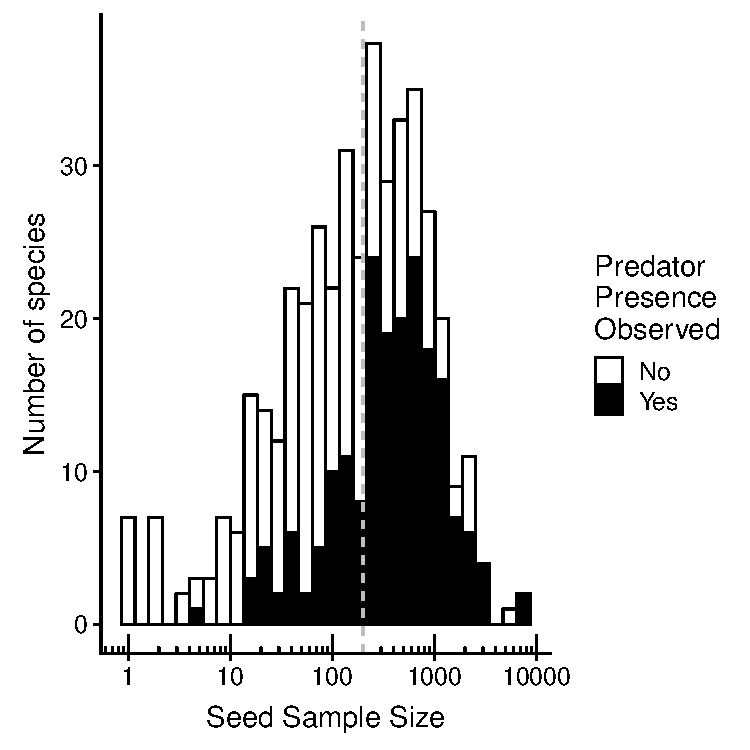
\includegraphics[width=0.7\textwidth]{../Figures/FigureS1.pdf} 
\caption[]{\textbf{Figure S1} Histogram showing the frequency distribution of sampling effort across the 478 collected plant species. The black portion of the bars represent species from which seed predators were reared. For species with few collected seeds, the likelihood of encountering seed predators was smaller than for species with larger sample sizes (logistic regression: $\beta$=0.0001, SE=0.0003, z=5.396, P<0.001). For species with sample sizes above 200 seeds (dashed line), the relationship between seed sample size and seed predator incidence was no longer statistically significant (logistic regression: $\beta$=0.0002, SE=0.0002, z=1.112, P=0.266).}
\end{figure}

\newpage

\section{Figure S2: Plant phylogeny including all plant species}

\begin{figure}[H]
\centering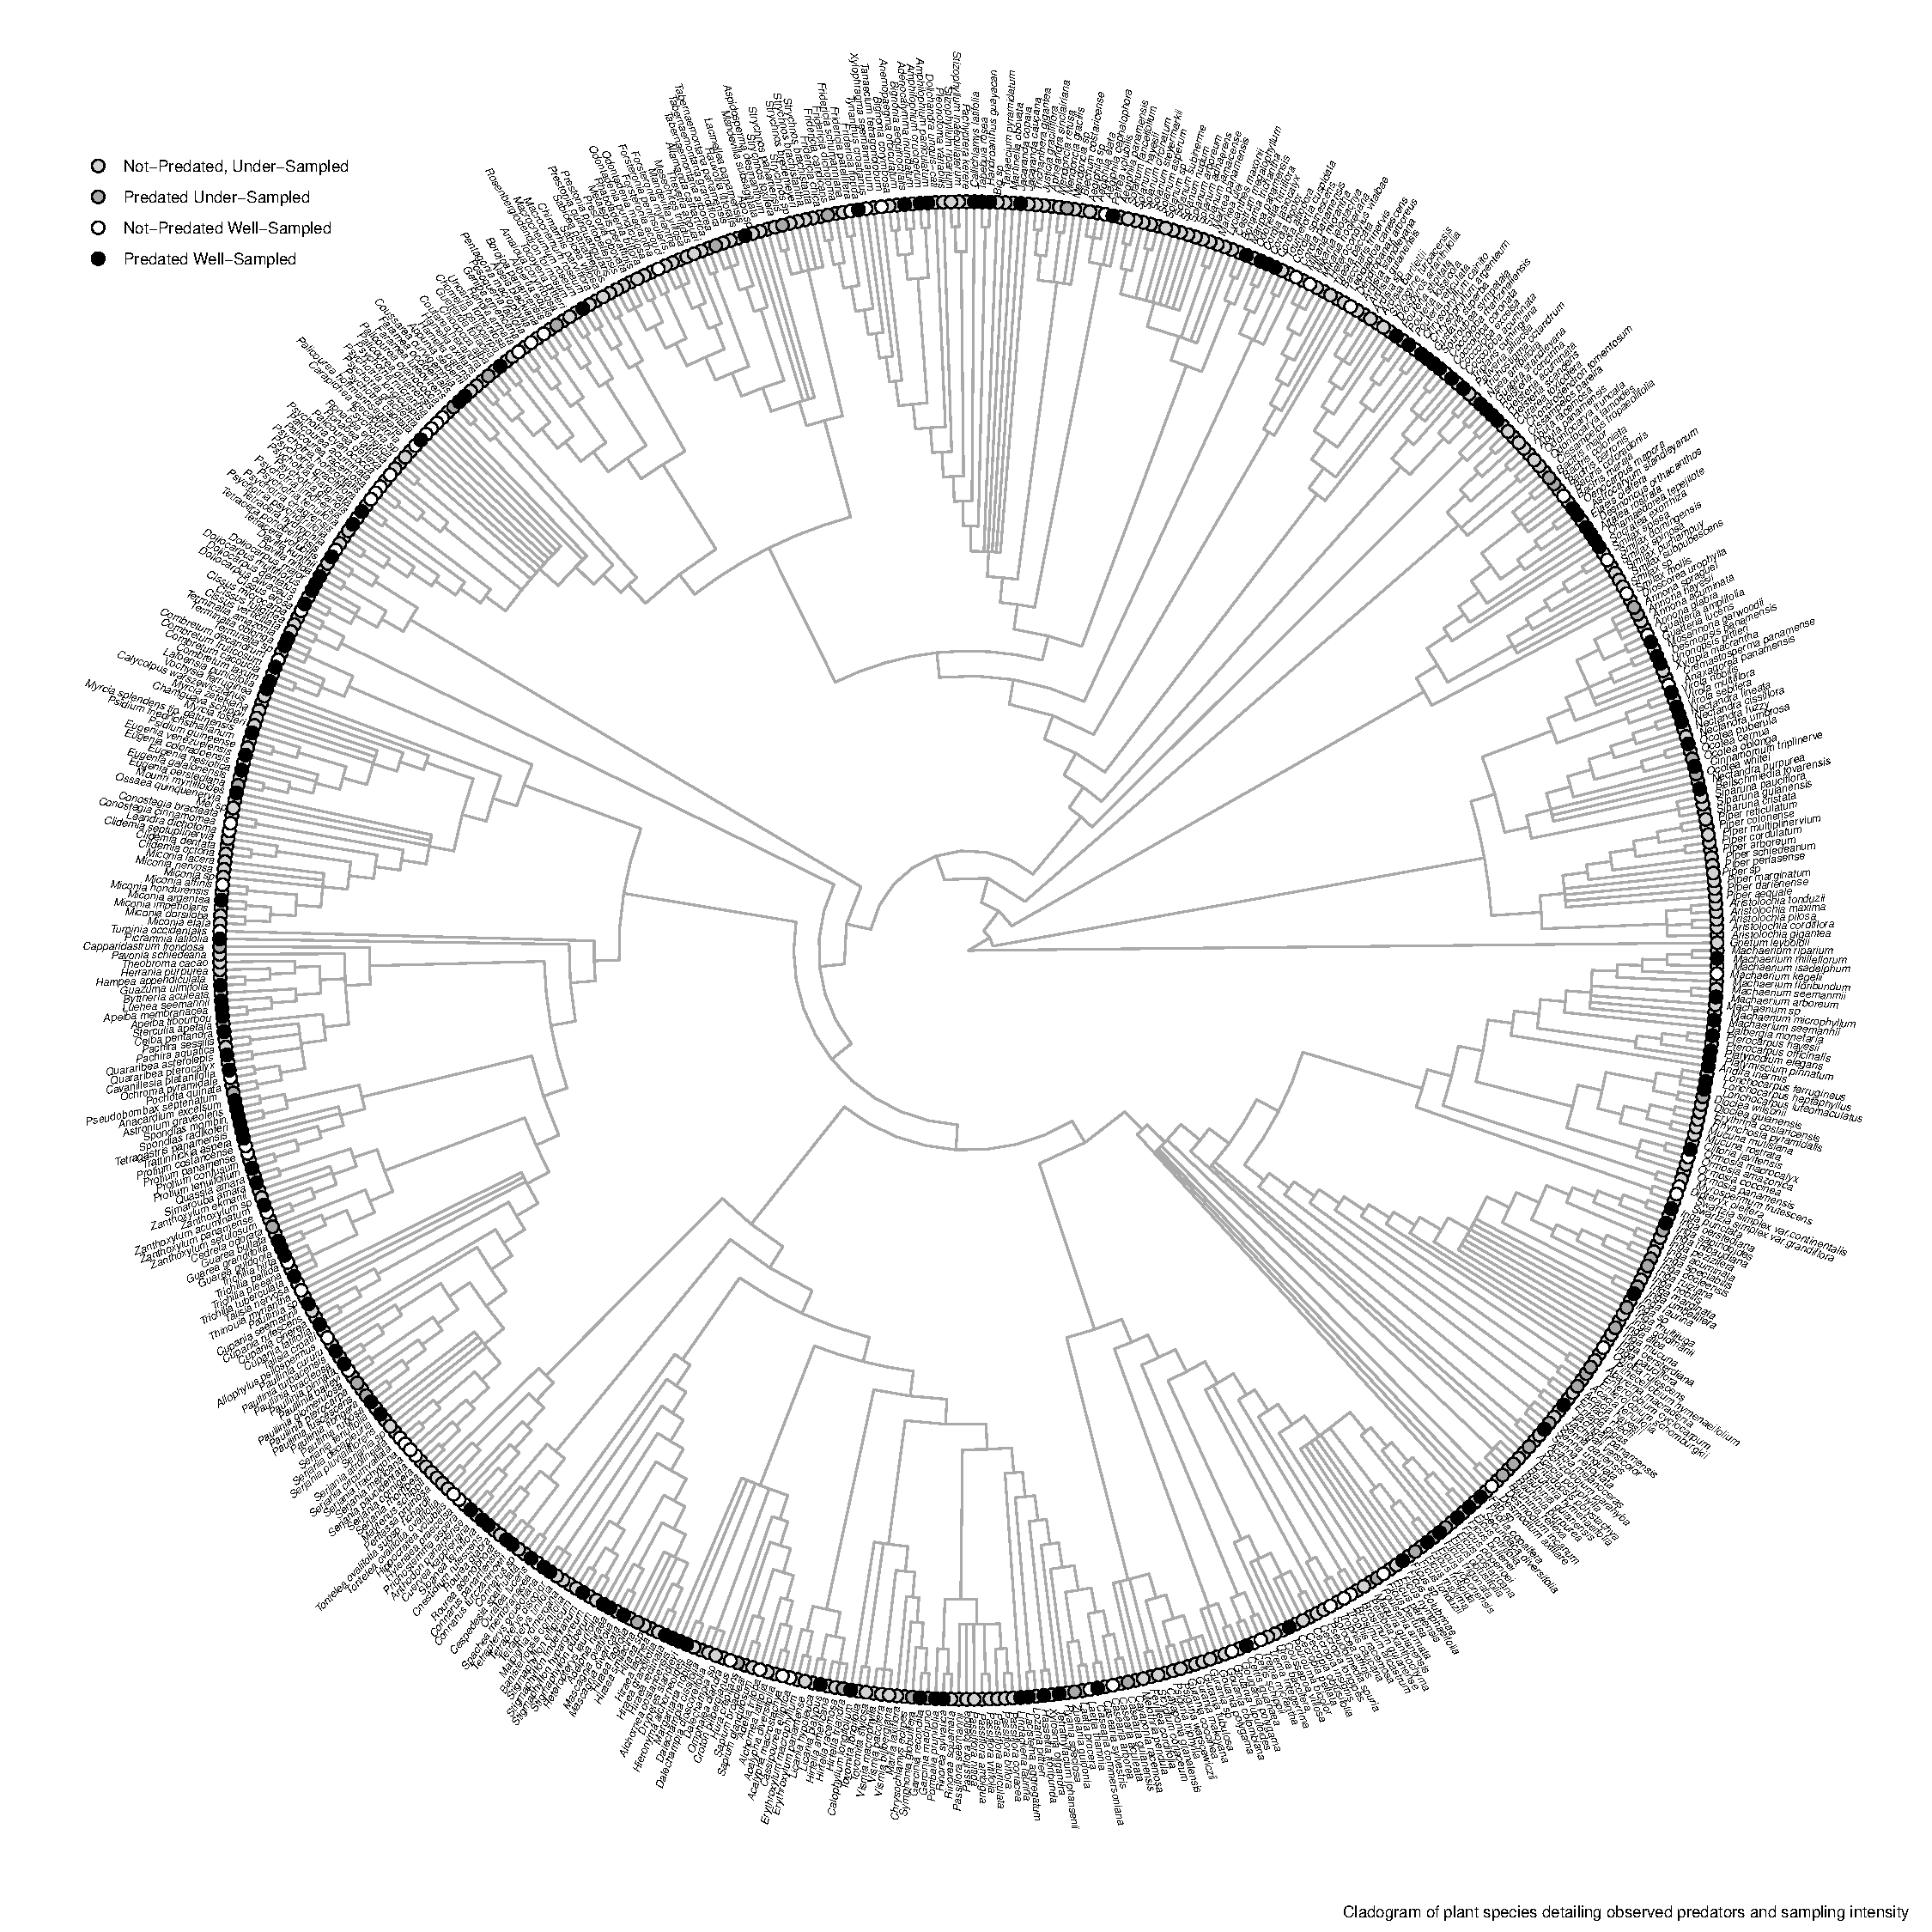
\includegraphics[width=\textwidth]{../Figures/FigureS2all.pdf} 
\caption[]{\textbf{Figure S2.} Presence or absence of seed predators (all orders combined) plotted against a plant phylogeny that includes all plant species sampled in this study for which phylogenetic information was available. The presence/absence of seed predators on well-samples plant species (minimum sample size of 200 seeds/fruits) is shown as black and white circles, respectively. For species with smaller sample sizes (<200 seeds/fruits) presence/absence of seed predators is shown as dark versus light grey circles. Of the 478 plant species for which seed samples were collected for insect rearing, 58 (12.1\%) could not be included in this figure because of lack of phylogenetic information.  }
\end{figure}

\newpage

\section{Figure S3: Spine plots depicting relationships between seed predator incidence and plant traits}

\begin{figure}[H]
\caption[]{\textbf{Figure S3.}  Spine plots depicting the relationships between seed predator incidence and the studied plant traits. The dark portion of the bars show the proportion of species within each trait category found to be attacked by one or more species of internally feeding insect seed predators. The width of each bar is proportionate to the number of plant species in the trait category.  }

\centering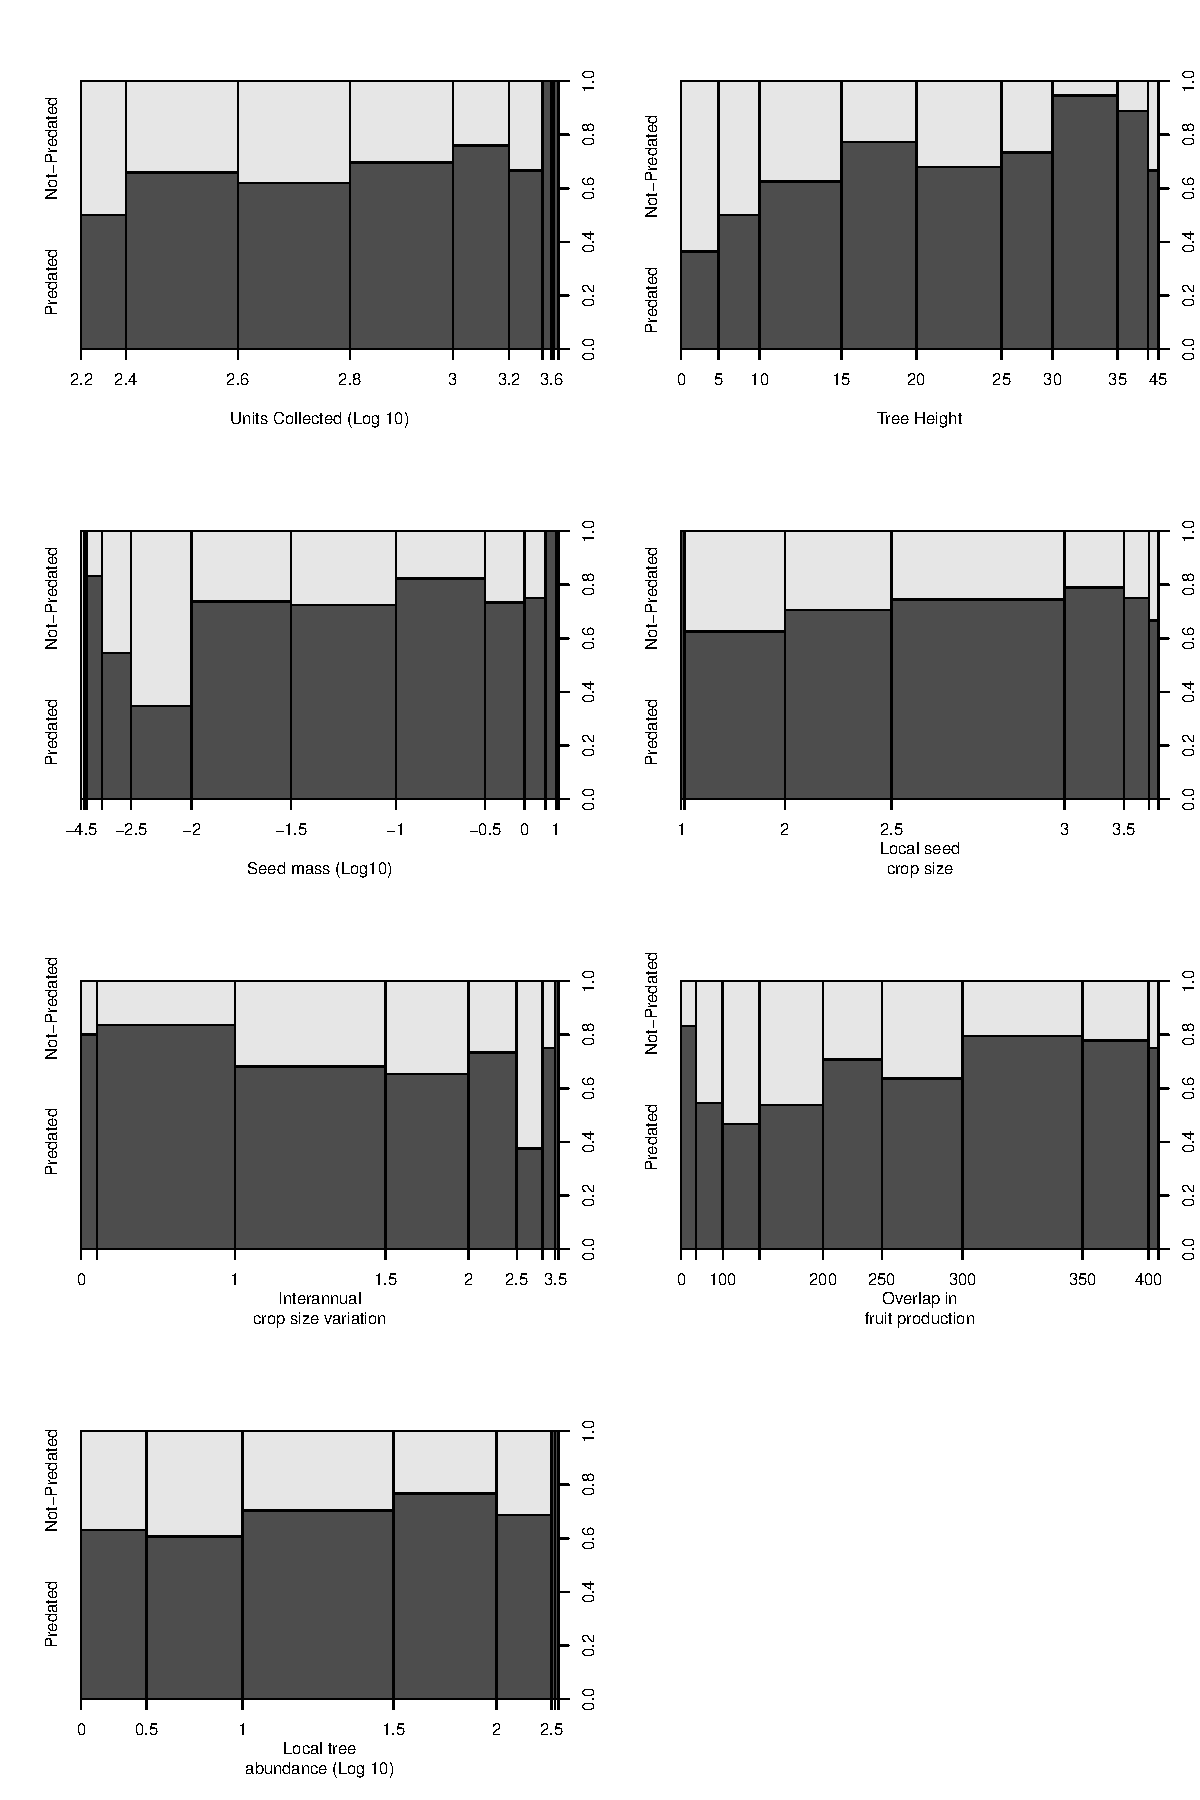
\includegraphics[width=0.7\textwidth]{../Figures/SpinePlotsa.pdf} 

\end{figure}
\newpage

\begin{figure}[H]
\centering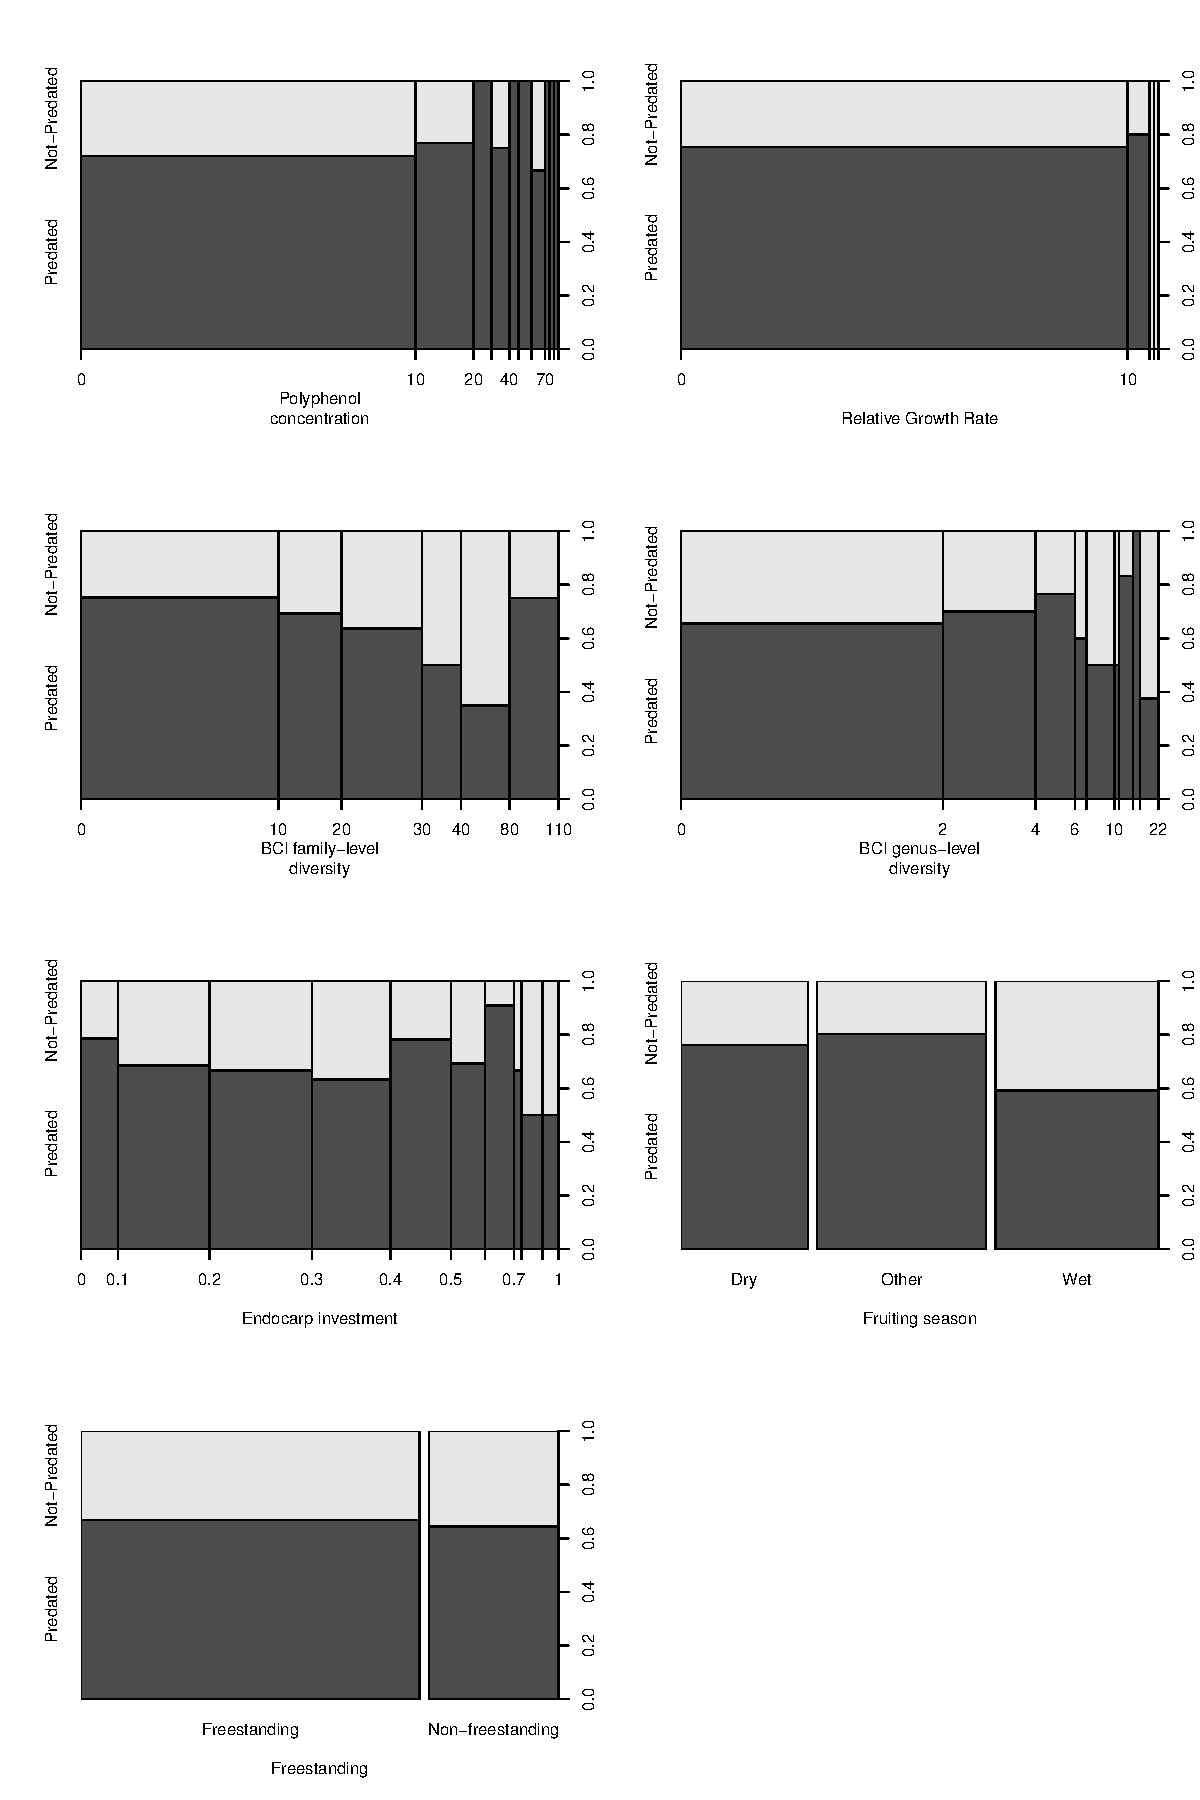
\includegraphics[width=0.7\textwidth]{../Figures/SpinePlotsb.pdf} 
\end{figure}

\newpage


\section{Figure S4: Quantitative food webs for Coleoptera and Lepidoptera}

\begin{figure}[H]
\caption[]{\textbf{Figure S4.} Quantitative food webs showing interactions between plants and their a) coleopteran and b) (overleaf) lepidopteran seed predators. For interpretation of the information in the food webs, see legend of Figure 4 in the main text.  }
\centering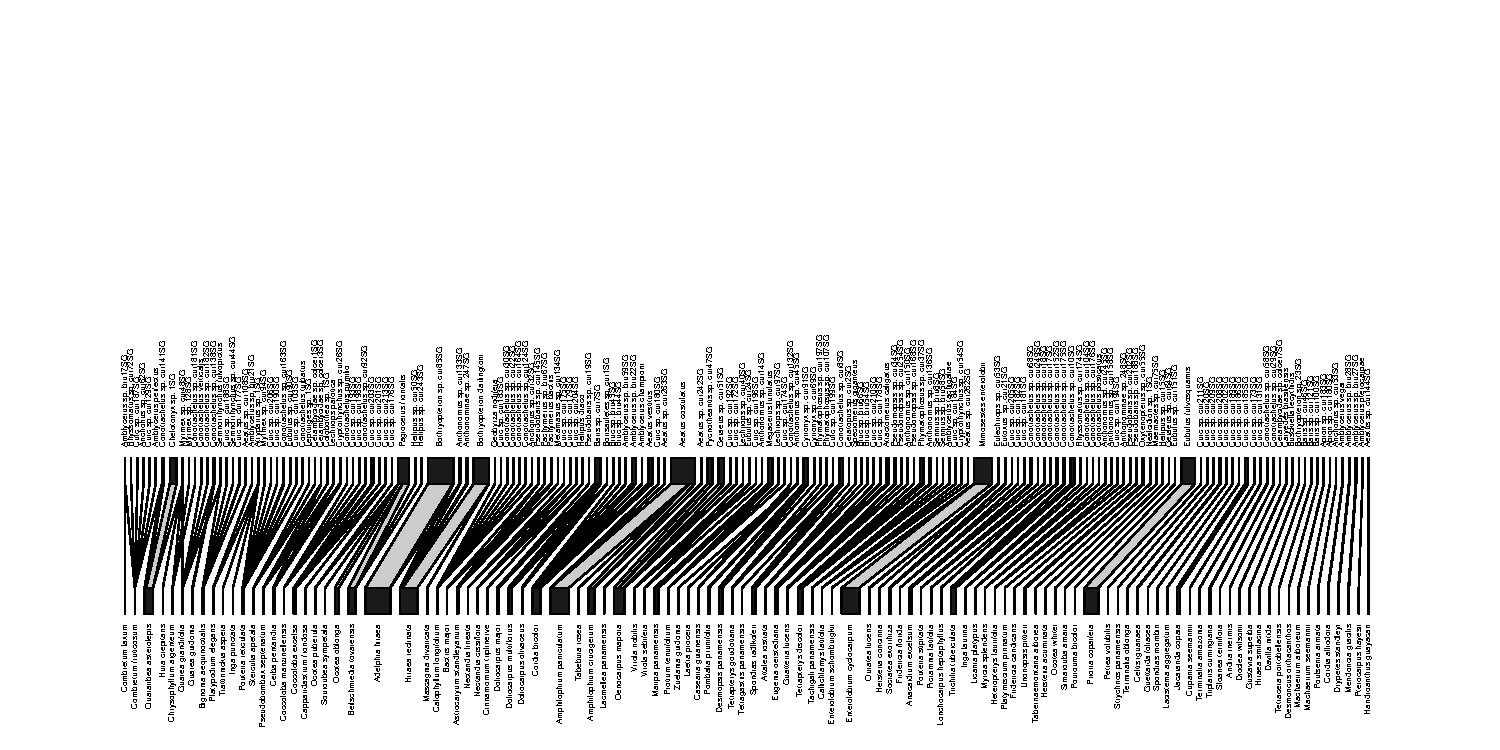
\includegraphics[width=1.2\textwidth, angle = 270, origin=c]{../Figures/FigureS4Coleoptera.pdf} 
\end{figure}

\begin{figure}[H]

\centering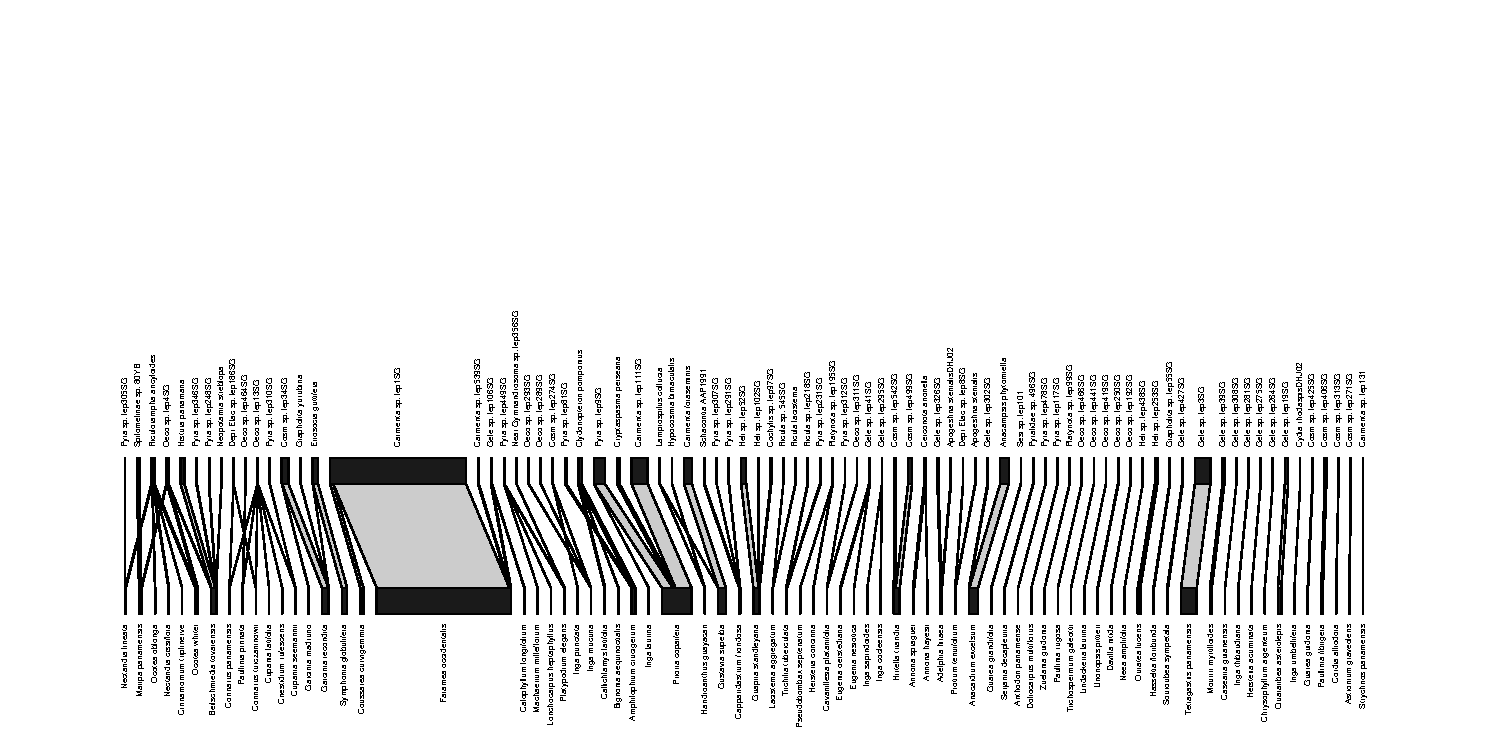
\includegraphics[width=1.2\textwidth, angle = 270, origin=c]{../Figures/FigureS4Lepidoptera.pdf} 

\end{figure}

\newpage


\section{Figure S5: Quantitative food web excluding singleton observations}


\begin{figure}[H]
\caption[]{\textbf{Figure S5.} Quantitative food web showing the interactions between seeds and their internally feeding seed predators. For interpretation, see legend of Figure 4 in the main text. In this version of the food web, singleton interactions (i.e. plant-seed predator interactions observed only once) have been excluded. }
\centering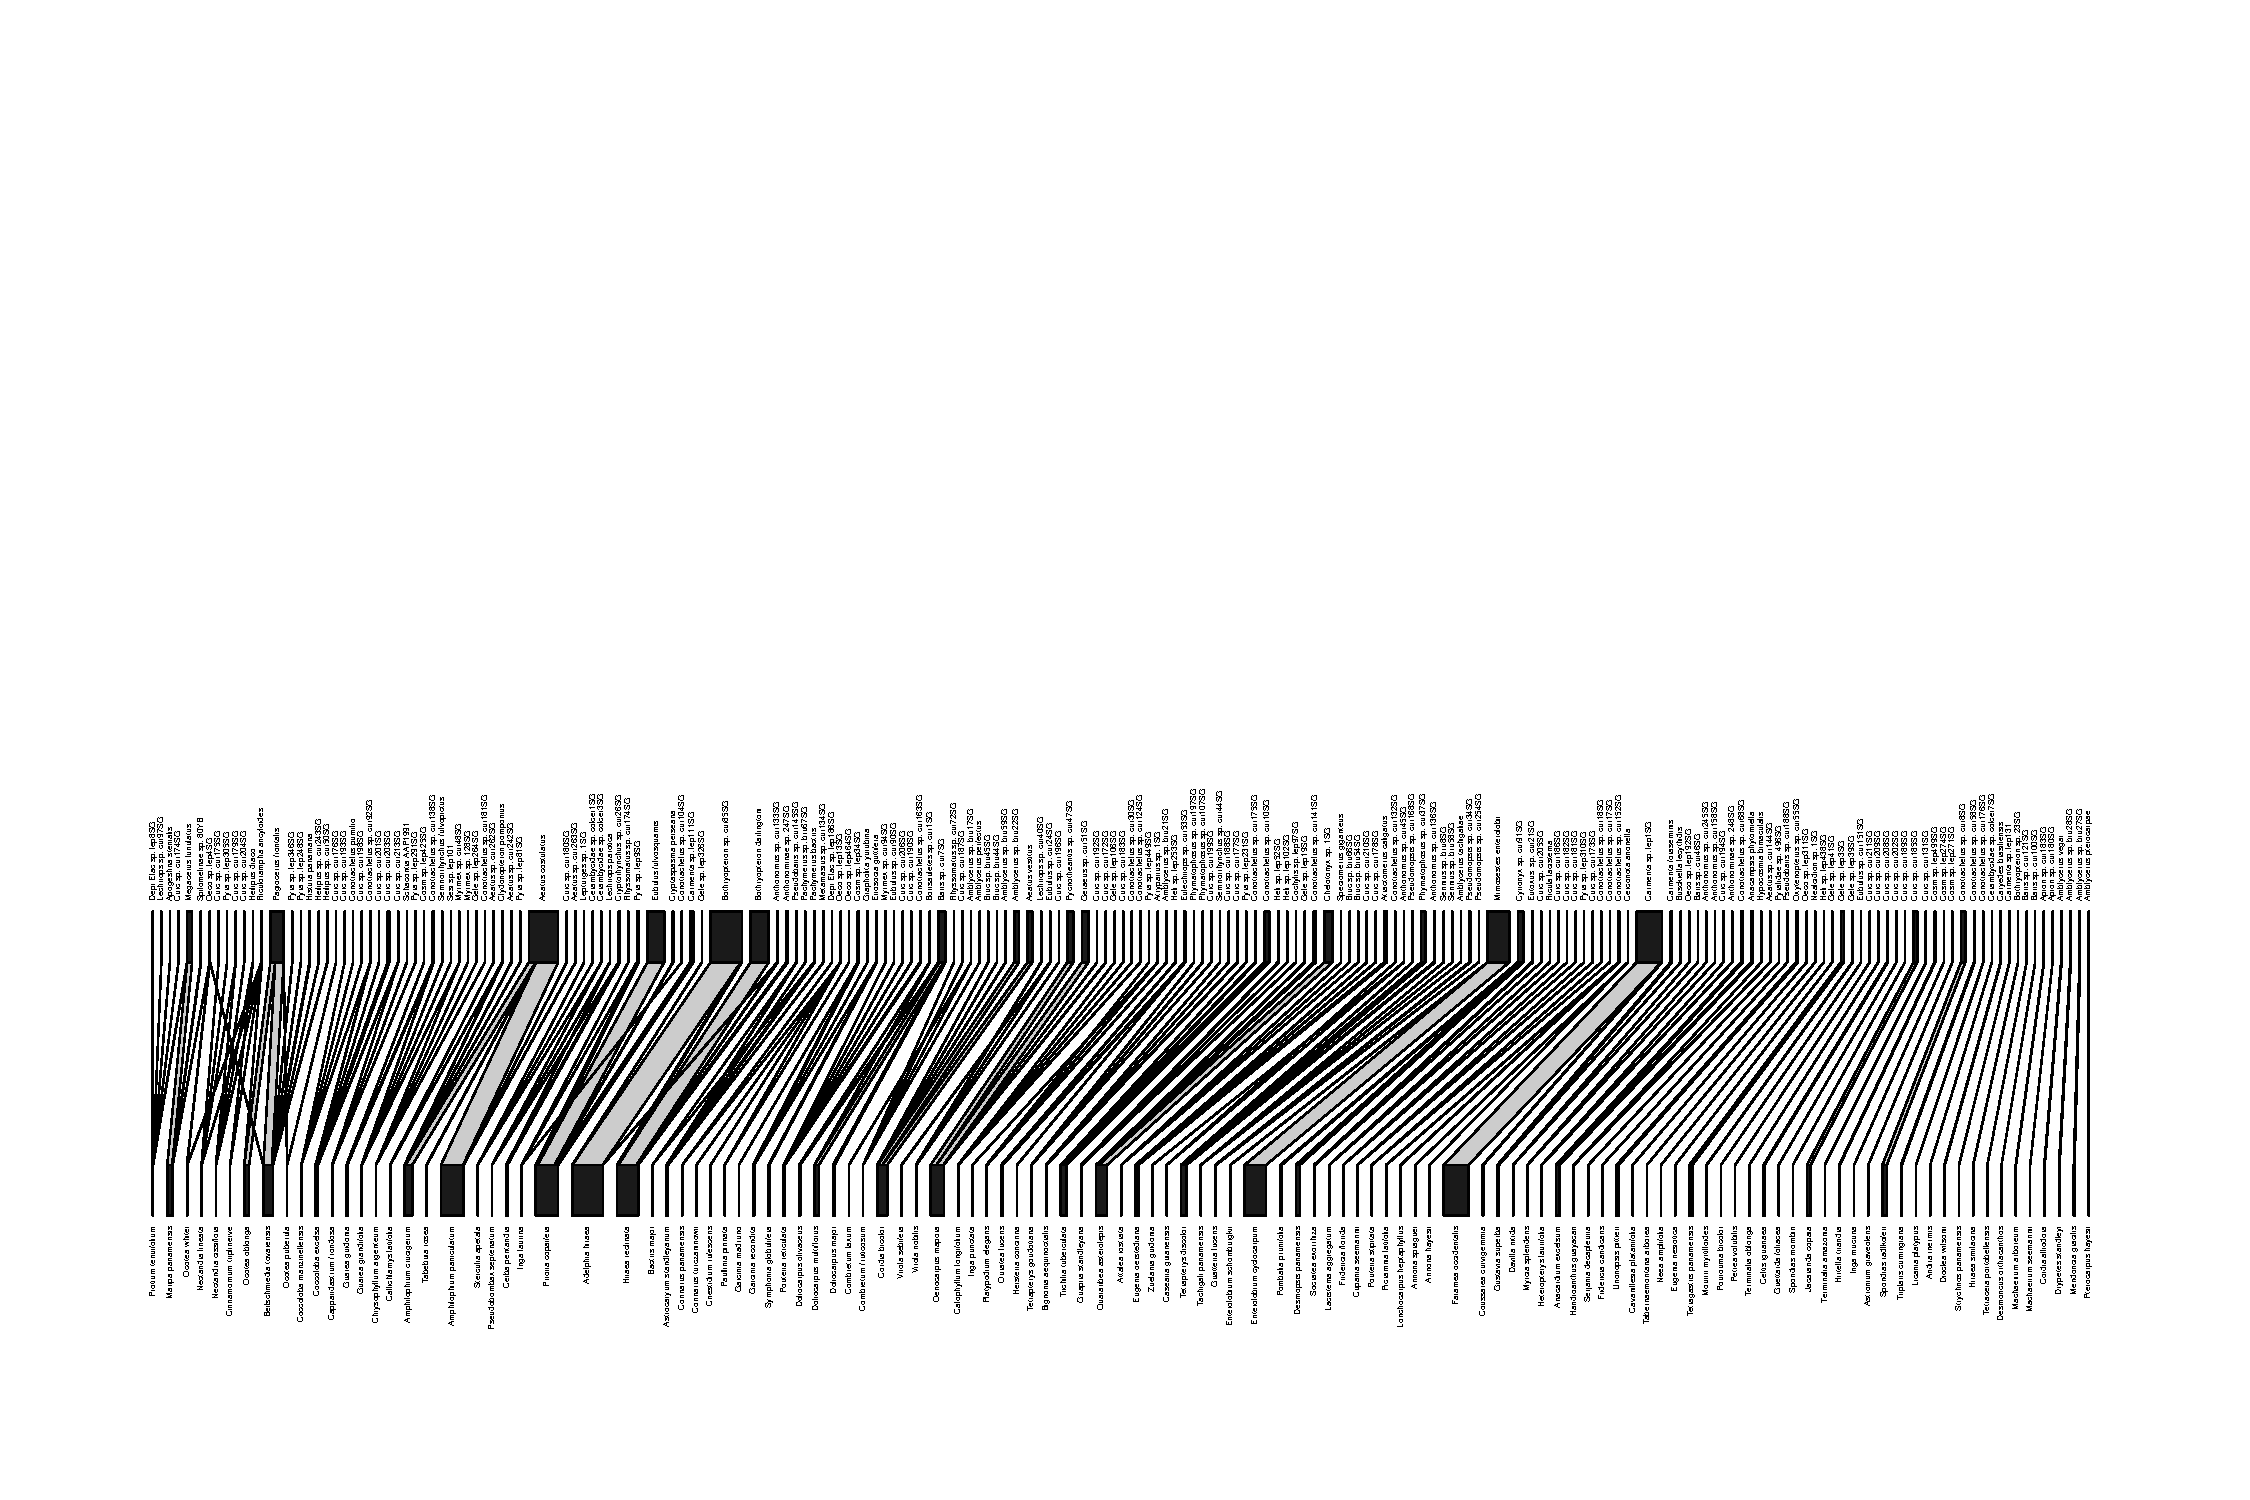
\includegraphics[width=1.2\textwidth, angle = 270, origin=c]{../Figures/FigureS5.pdf} 
\end{figure}


\newpage


\section{ Figure S6: Relationship between potential for apparent competition and phylogenetic distance}


\begin{figure}[H]
\caption[]{\textbf{Figure S6.} Potential for indirect interactions (as assessed using the PAC index; see main text) plotted against the phylogenetic distance between pairs of plant species. Shown are only cases where PAC>0. The red line is a trend line obtained from a linear model, and used for the purposes of plotting only (to visualise patterns in the relationship between PAC and pairwise phylogenetic distances).}
\centering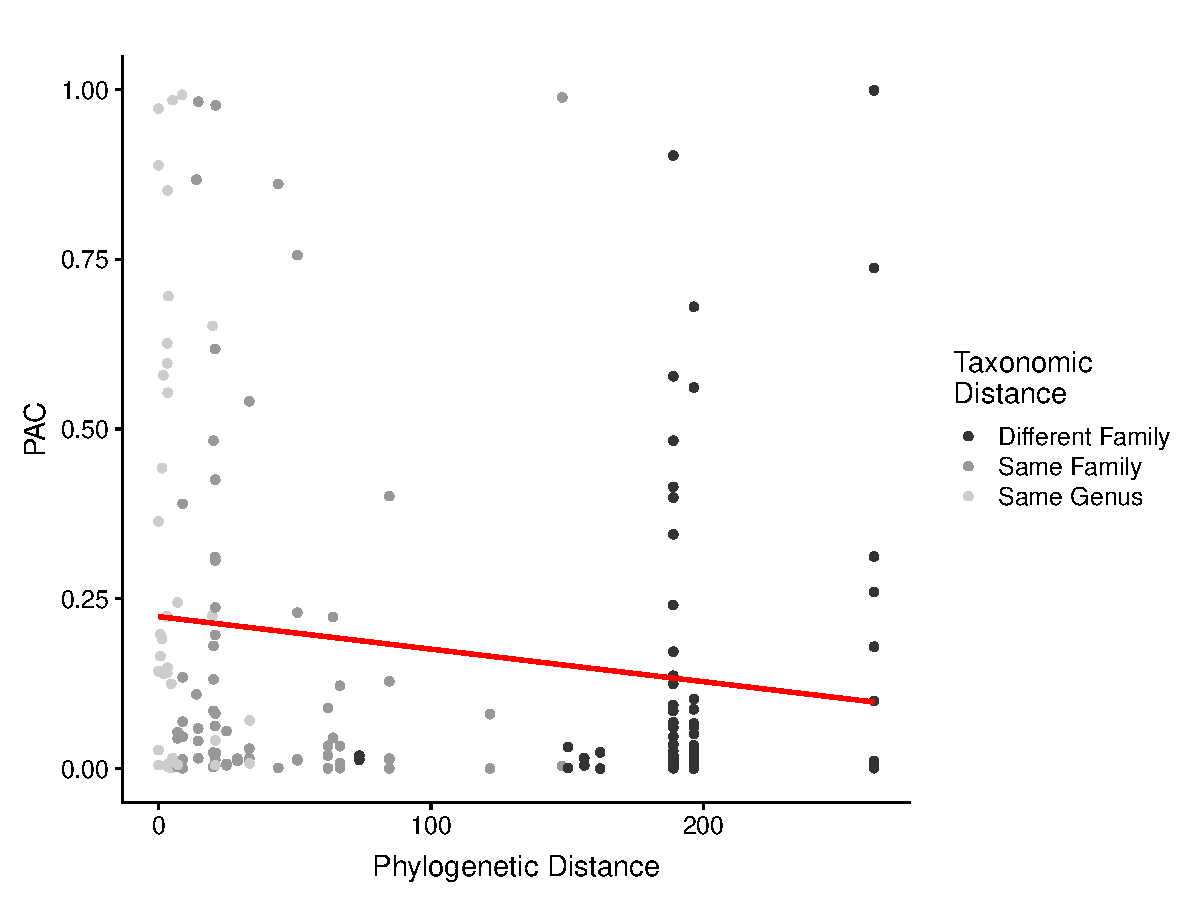
\includegraphics[width=0.7\textwidth]{../Figures/FigureS6.pdf} 
\end{figure}



\end{document}
